\chapter{Simulation}
\label{sec:SimulationResults}
Two levels of simulation are discussed in this section; first of single voxels,
and second of a single slice (64x64 voxels).  The single time series tests
investigate the ability of particle filters to estimate parameters of the BOLD model 
in a noisy environment. Single voxel tests were
performed eleven different times, each with a new noise realization.
Repeating tests with different noise realizations demonstrates the 
particle filter's resiliance to noise and explores the variance of
the model. 

The slice simulation was performed using 
Physics-Oriented Simulated Scanner for Understanding MRI (POSSUM) which
models noise realistically. POSSUM demonstrates the 
particle filter modeling the BOLD signal on a large scale. 
In the POSSUM simulation there were four
discrete parameter sets driving the timeseries, although each voxel had a 
different tissue composition and a different
noise realization. Therefore the POSSUM simulation was 
a good test of the applicability of particle filters for performing
whole brain analysis. 

Note that except for \autoref{sec:VeryLongSim} the same stimulus sequence
that was used in real data (\autoref{sec:RealData}) was used in the simulations. This sequence may
be found in \autoref{sec:ExperimentConfig}, but because of the availability of ground
truth in simulations is not displayed in this section.

\section{Single Time Series}
\label{sec:Single Voxel Simulation}
Given the state-space equations for the BOLD signal, simulating a single time 
series was straight forward. After generating a true signal,
identically and independently distributed (I.I.D.) Gaussian noise and a Wiener
process with Gaussian I.I.D. steps were added to the true signal. Finally a 
carrier level was added, since BOLD is typically
measured as a \% difference from the baseline. The particle filter
algorithm immediately removes this by calculating the \% difference, 
but adding a carrier level meant that the exact same algorithm used 
for simulated data could be used for the real data. 

Once this noisy simulated time series was generated, the particle filter algorithm
was run on the single time series image. Five sets of tests 
determine the power of the particle filter in modeling. 
The first test demonstrates the particle filter on a very long FMRI
run, and discusses the inherent learn-ability of the BOLD model 
(\autoref{sec:VeryLongSim}). 
The next two (\autoref{sec:SimLowNoise} and \autoref{sec:SimHighNoise}) 
demonstrate the ability of the particle filter to find the most likely
set of parameters/state variables over the course of a run identical to the
real run in \autoref{sec:RealData}. The last two 
tests (\autoref{sec:PureNoiseLowMag} and \autoref{sec:PureNoiseHighMag}) 
investigate the problem of false-positives. As the first
round of tests show, given the presence of an underlying BOLD signal, 
the particle filter is excellent at finding the most probable cause of 
the observed signal. As discussed in \autoref{sec:PureNoiseLowMag} and 
\autoref{sec:PureNoiseHighMag}, even when there is no underlying signal, 
the particle filter may still converge. Because of this problem, it was 
necessary to investigate methods of identifying false positives.

\subsection{Ideal Analysis}
\label{sec:VeryLongSim}

\begin{figure}
\centering
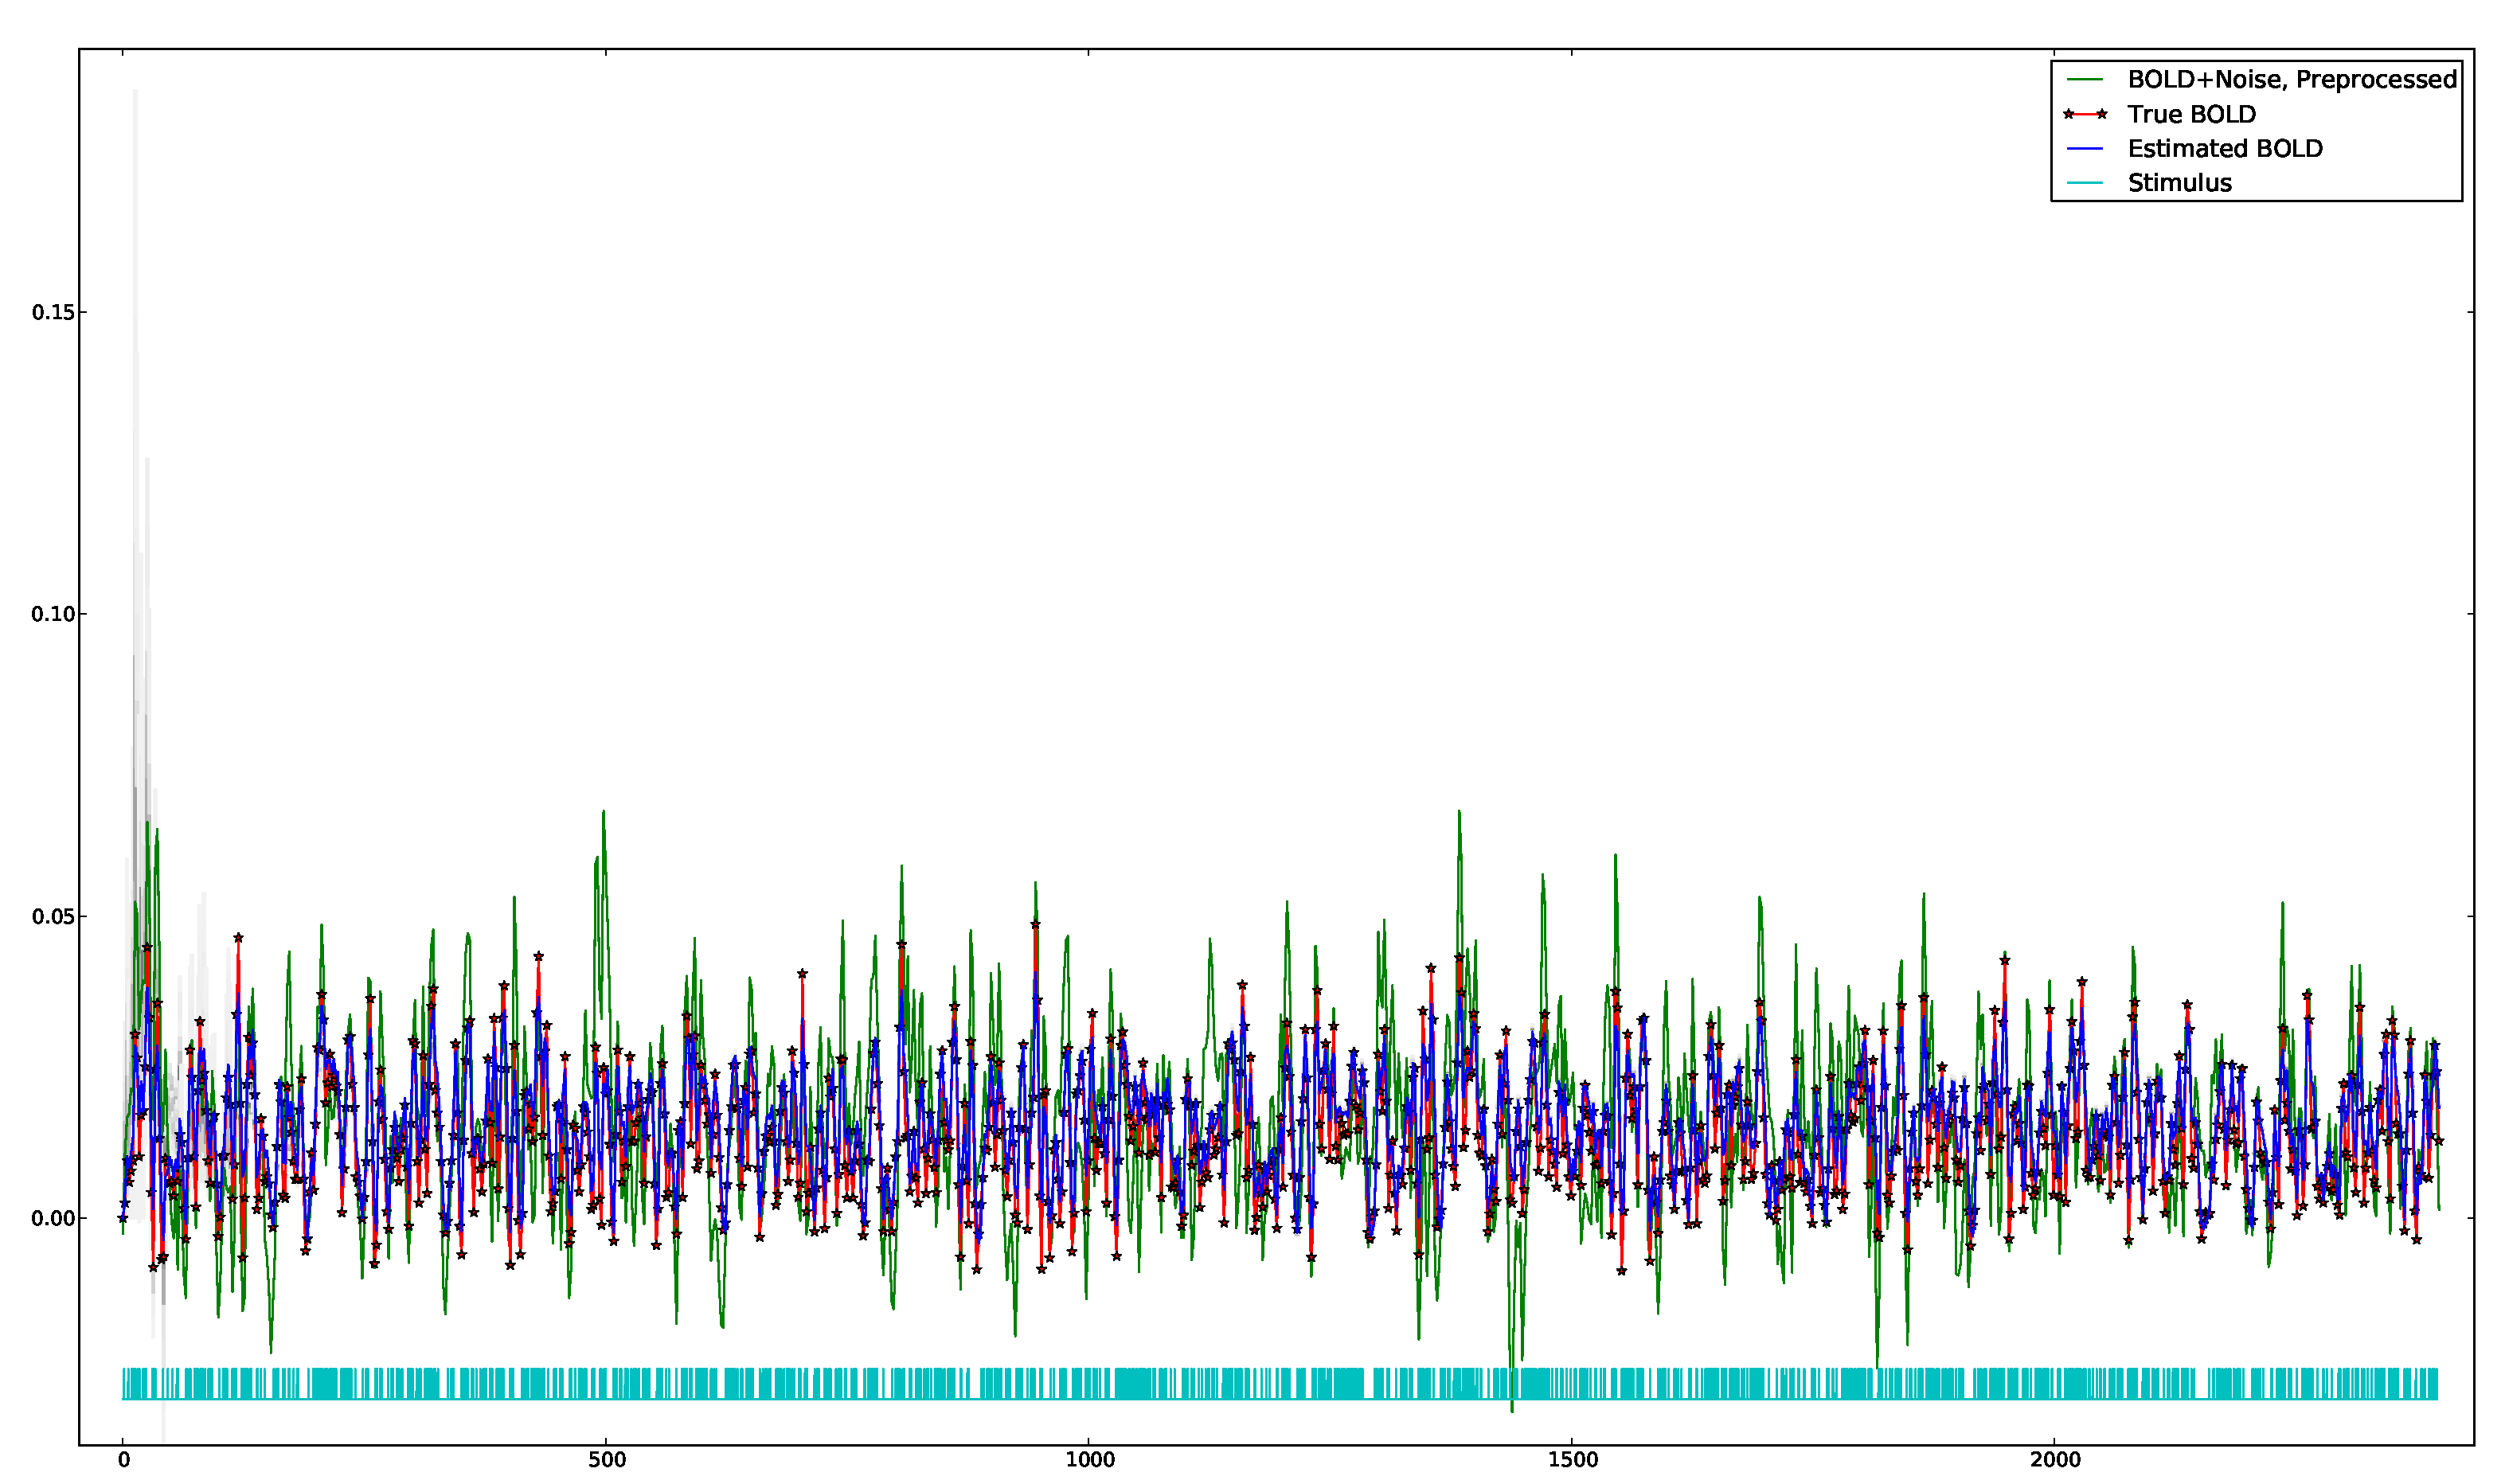
\includegraphics[clip=true,trim=1cm 0cm 0cm 0cm, width=17cm]{images/long_converge}
\caption{BOLD estimate converging for a very long FMRI run. Darker bars indicate
bins with more regions. }
\label{fig:long_converge}
\end{figure}

\begin{figure}
\centering
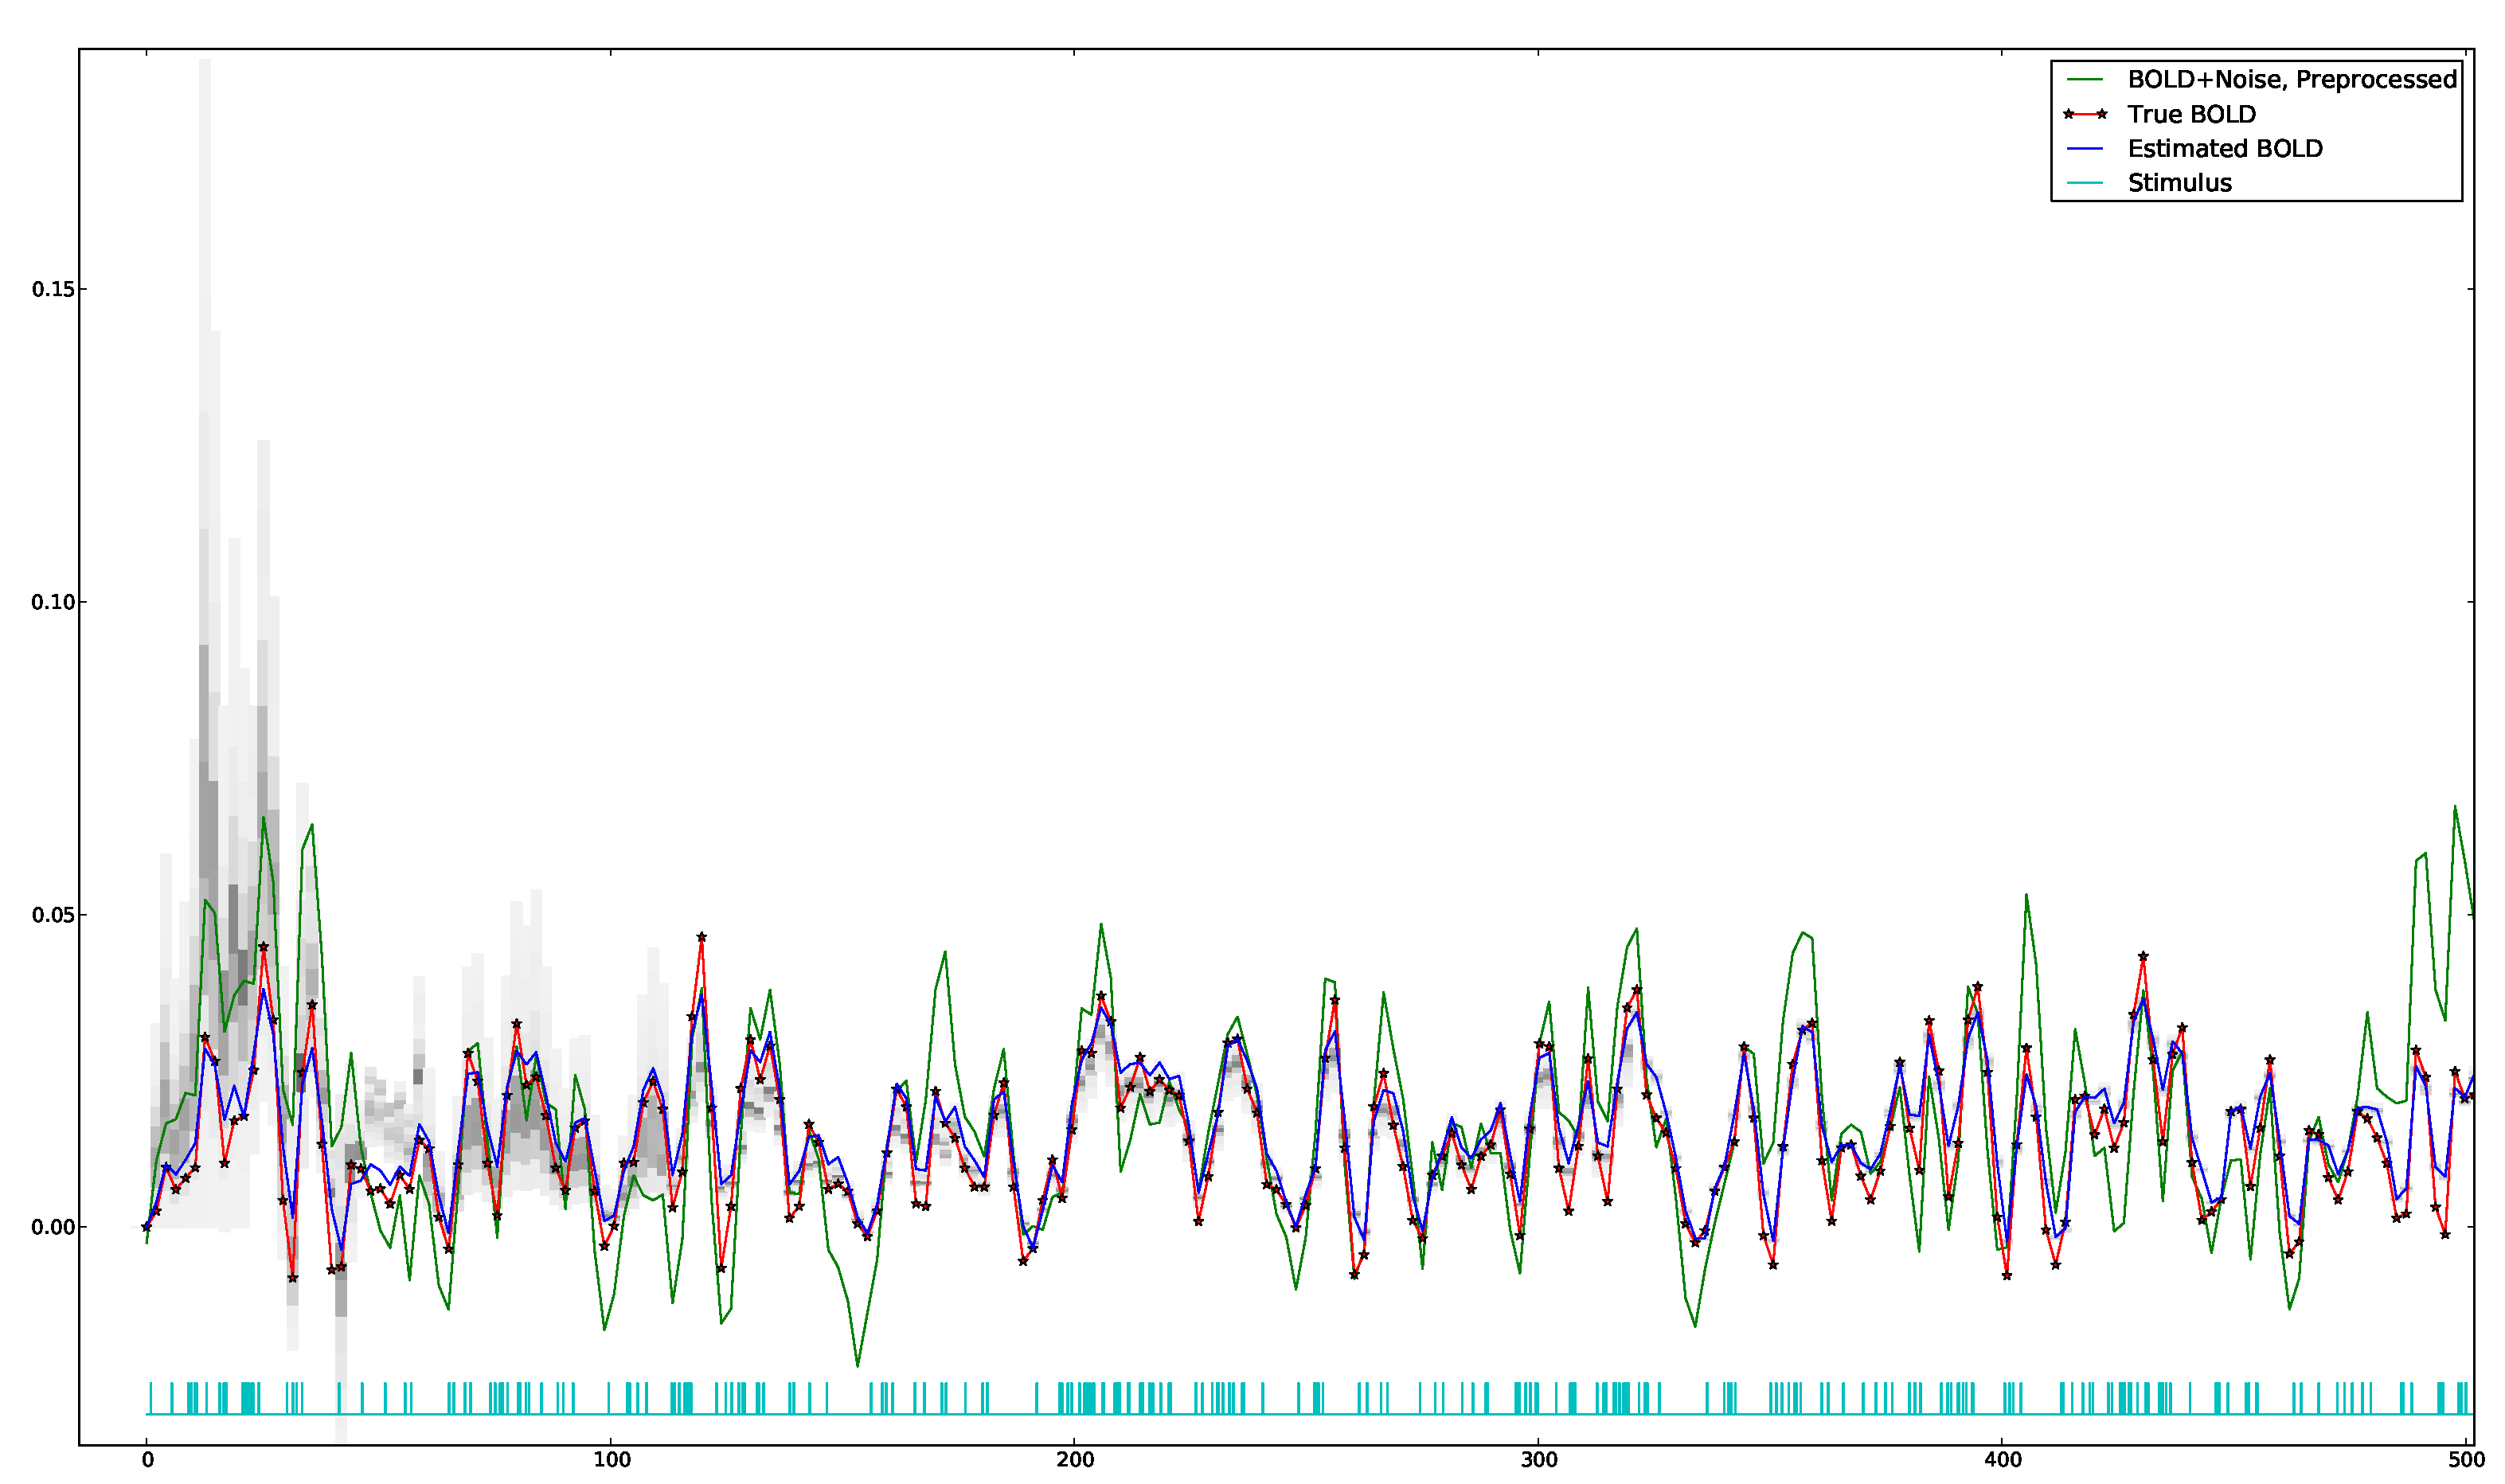
\includegraphics[clip=true,trim=1cm 0cm 0cm 0cm, width=17cm]{images/long_converge_500}
\caption{BOLD estimate converging for a very long FMRI run, first 500 seconds. Darker bars
indicate bins with more particles.}
\label{fig:long_converge_500}
\end{figure}

\begin{table}[t]
\begin{tabular}{|c | c  c  c  c  c  c  c |}
\hline 
  & $\tau_0$ & $\alpha$ & $E_0$    & $V_0$    & $\tau_s$ & $\tau_f$ & $\epsilon$ \\
\hline 
\rowcolor[gray]{.8} $\tau_0$  & 0.0004334 & 5.2e-05 & -6.95e-05 & 3.3e-06 & 0.0001628 & -2e-07 & 0.0001798 \\
$\alpha$                      & 5.2e-05 & 7.9e-06 & -6.4e-06 & 3e-07 & 1.04e-05 & -1.92e-05 & 2.58e-05 \\
\rowcolor[gray]{.8} $E_0$     & -6.95e-05 & -6.4e-06 & 1.9e-05 & -9e-07 & -4.11e-05 & -3.24e-05 & -3.92e-05 \\
$V_0$                         & 3.3e-06 & 3e-07 & -9e-07 & 1e-07 & 1.1e-06 & 9e-07 & 1e-06 \\
\rowcolor[gray]{.8} $\tau_s$  & 0.0001628 & 1.04e-05 & -4.11e-05 & 1.1e-06 & 0.0001589 & 0.0001518 & 7.88e-05 \\
$\tau_f$                      & -2e-07 & -1.92e-05 & -3.24e-05 & 9e-07 & 0.0001518 & 0.0002966 & -2.34e-05 \\
\rowcolor[gray]{.8} $\epsilon$& 0.0001798 & 2.58e-05 & -3.92e-05 & 1e-06 & 7.88e-05 & -2.34e-05 & 0.0001966 \\
\hline 
\end{tabular}
\caption{Covariance matrix of the parameters at the end of \autoref{fig:long_converge}.}
\label{tab:long_cov} 
\end{table}

\begin{table}[t]
\begin{tabular}{|c | c  c  c  c  c  c  c |}
\hline 
  & $\tau_0$ & $\alpha$ & $E_0$    & $V_0$    & $\tau_s$ & $\tau_f$ & $\epsilon$ \\
\hline 
\rowcolor[gray]{.8} $\tau_0$  & & & & & & & \\
$\alpha$                      & 0.889884 & & & & & & \\
\rowcolor[gray]{.8} $E_0$     & -0.7661395 & -0.5230723 & & & & & \\
$V_0$                         & 0.6244049 & 0.4239271 & -0.7964774 & & & & \\
\rowcolor[gray]{.8} $\tau_s$  & 0.6204843 & 0.295425 & -0.7481253 & 0.3440421 & & & \\
$\tau_f$                      & -0.0004259 & -0.3966881 & -0.4314174 & 0.1962954 & 0.6990775 & & \\
\rowcolor[gray]{.8} $\epsilon$& 0.6158116 & 0.6558179 & -0.641348 & 0.2846632 & 0.4458142 & -0.097079 & \\
\hline 
\end{tabular}
\caption{Correlation of parameter estimates at the end of \autoref{fig:long_converge}.}
\label{tab:long_corr} 
\end{table}

To begin the single voxel simulation; I generated a signal using the following parameters:
$\{\tau_0 = 1.45, \alpha = 0.3, E_0 = 0.47, V_0 = 0.044, \tau_s = 1.94, \tau_f = 1.99, \epsilon = 1.8\}$.
These same parameters were used throughout this chapter. Noise
was generated based on measurement noise ($\sigma_y$) of $0.001$ and drift standard deviation
($\sigma_x$) of $0.0005$. The measurement noise as well as the steps of the drift
were taken to be Gaussian. The actual signal delivered into the particle filter
was the result of preprocessing to remove drift, as described in 
\autoref{sec:Methods Preprocessing}. 

To test how well the particle filter would do with plenty of data, and 
determine the inherent variance in the model parameters, a very long simulation
with randomly generated impulse stimuli was created. The preprocessed timeseries
and the final estimate are shown in \autoref{fig:long_converge};
the final covariance matrix of the parameters is in \autoref{tab:long_cov}.
Note that even though the BOLD response converged well (\autoref{fig:long_converge}),
the parameters still have significant correlation (\autoref{tab:long_corr}). 
Based on the histograms in the first 500 seconds, the parameters converged to
their final values well before the end.
Although this is only a single test, the correlation (\autoref{tab:long_corr}) 
of the parameters 
indicates significant parameter indeterminability. When the input
consists entirely of impulses, the best parameters are not one particular
set, but a spectrum. Note that the correlation is in parameters whose priors
are completely independent. It is possible that varying the type of input could
give improved results, although informal tests did not show significant difference.
In spite of the noisy input (green line in \autoref{fig:long_converge}), the estimates
of the BOLD were actually very close to the true (noise-free) BOLD signal.

%LOW NOISE SECTION, with a signal
\subsection{Simulation with Low Noise}
\label{sec:SimLowNoise}
%tests had noise of $ \{\sigma_y = .01, \sigma_x = .005\} $, where $\sigma_y$ is the
%measurement noise, and $\sigma_x$ is the wiener step size. Both signals used the
%parameters .
%The particle filter used the parameters defined in \autoref{tab:Prior} (\autoref{sec:PriorDistrib}),
%thus the particle filter was not centered over the correct values. 
\begin{figure}
\centering
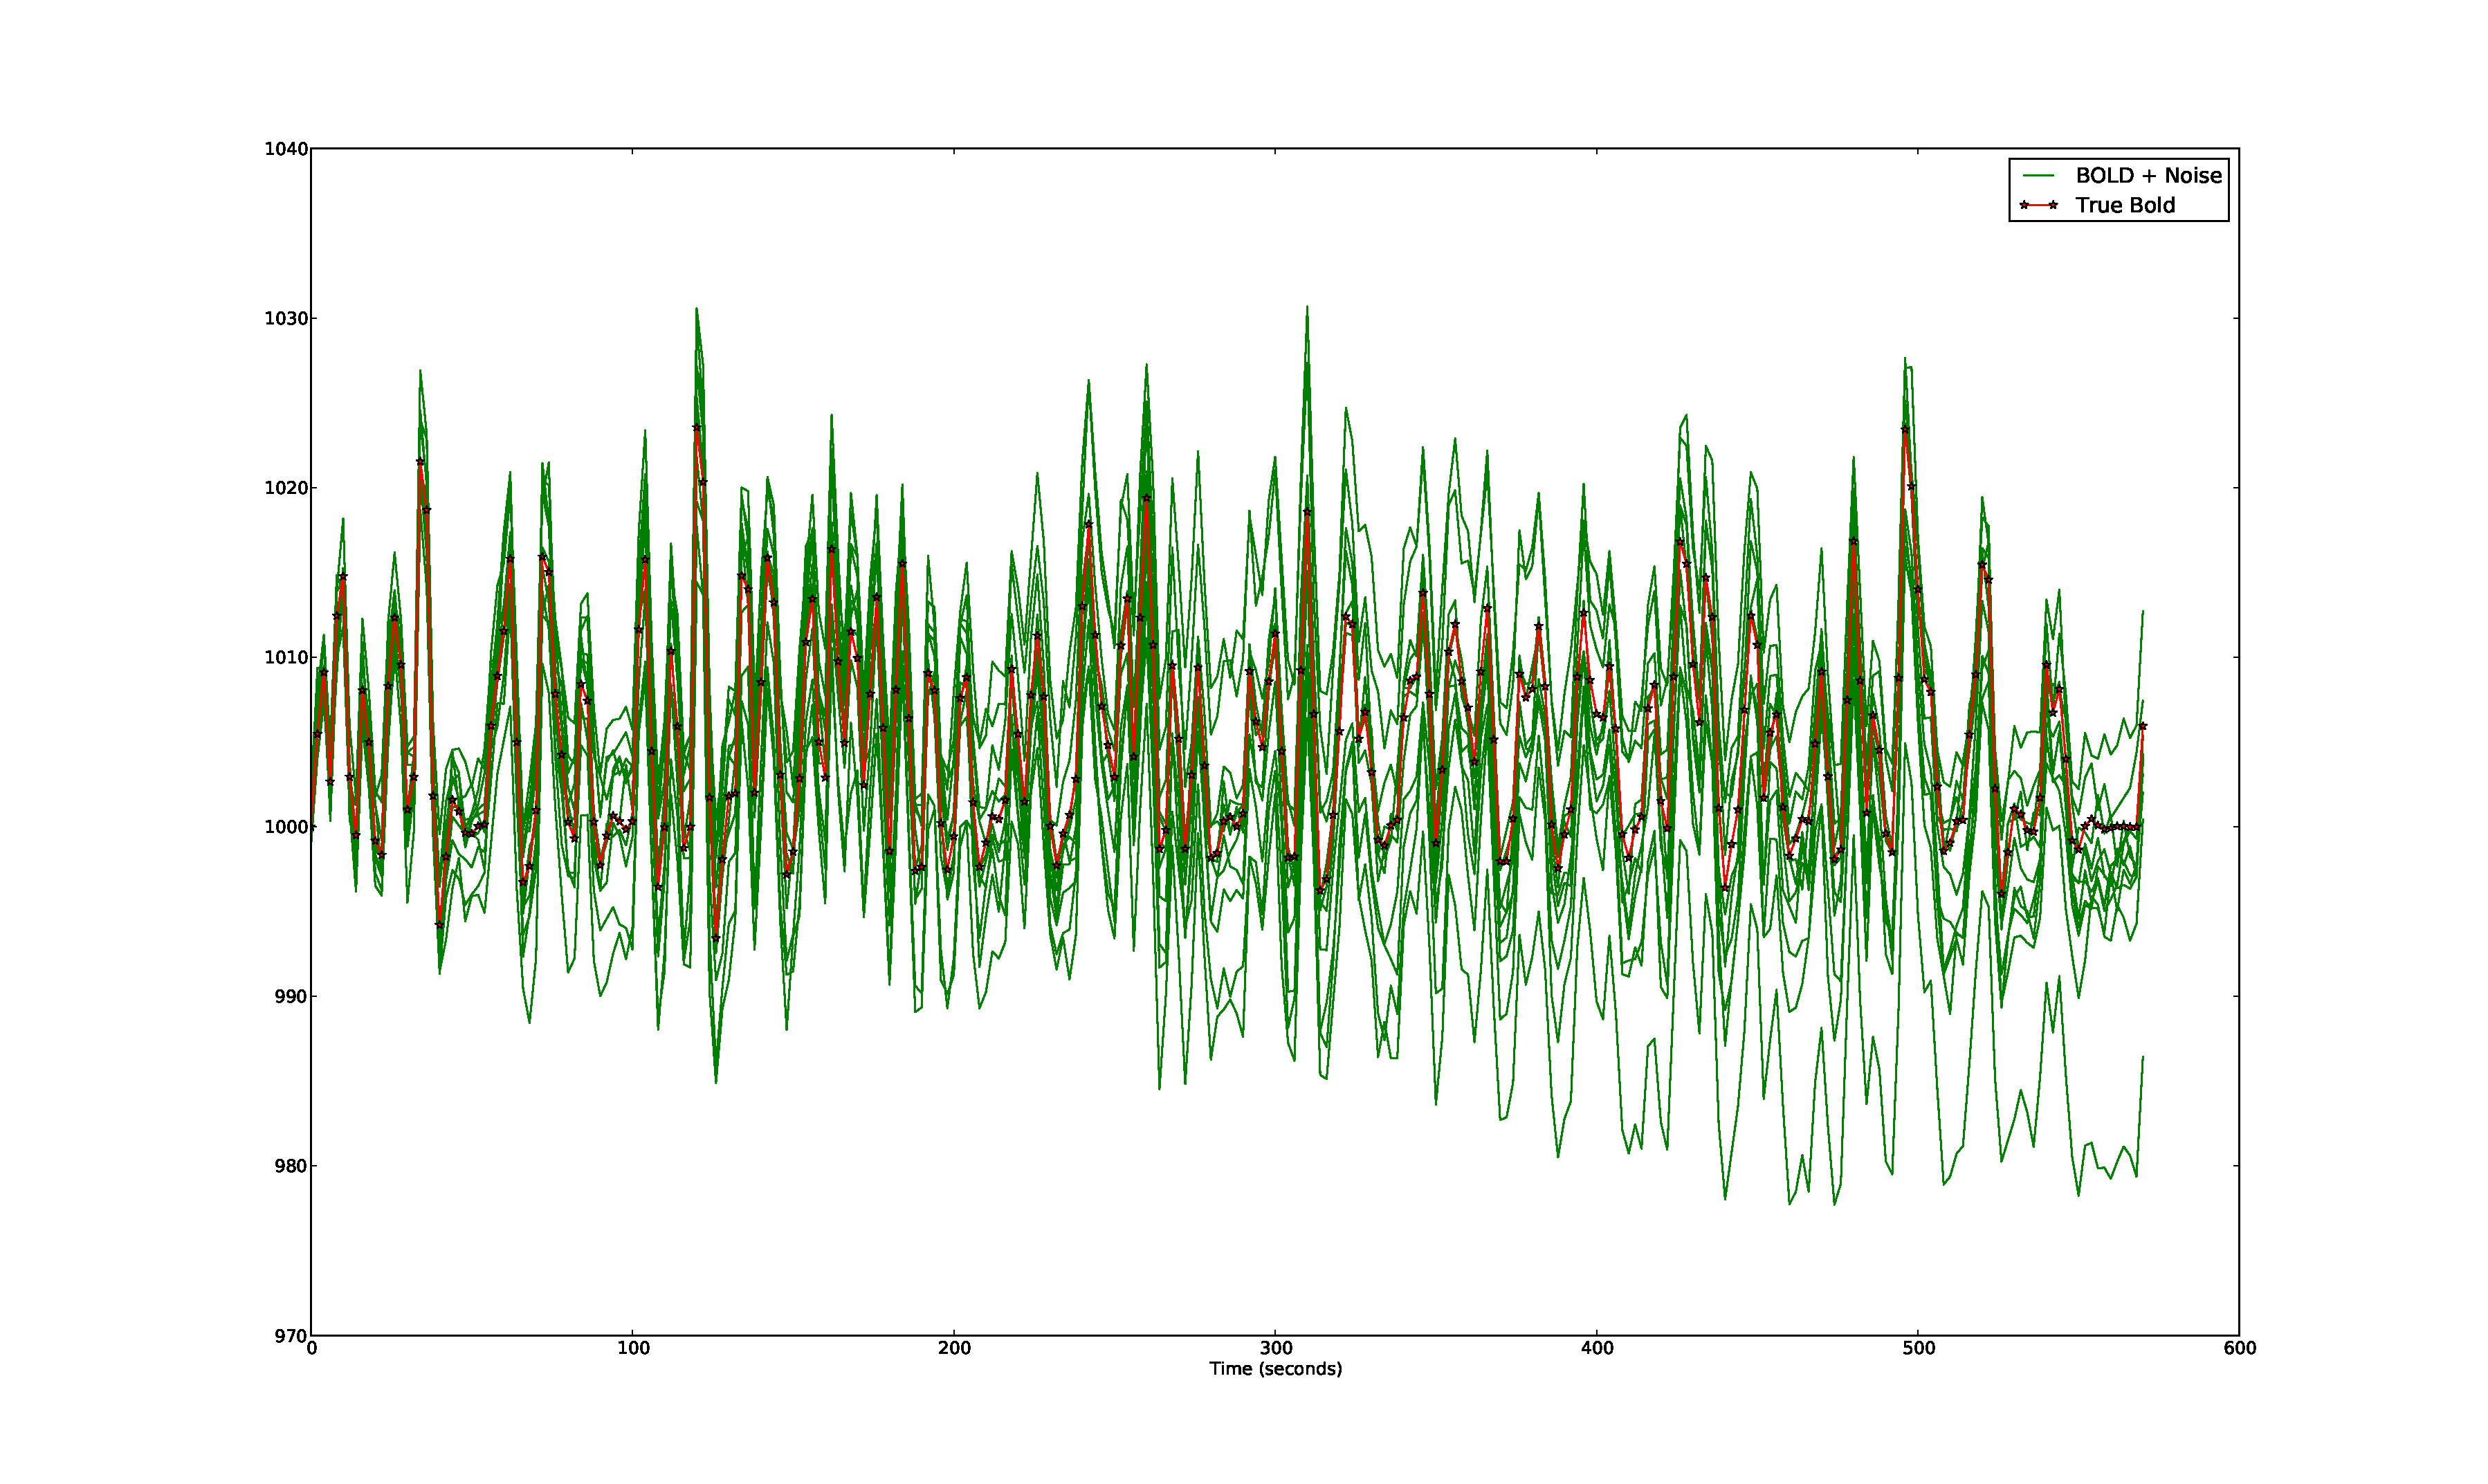
\includegraphics[clip=true,trim=6cm 2cm 5cm 3.5cm,width=15cm]{images/realization_lownoise}
\caption{Test Signals with low noise compared to the clean signal.}
\label{fig:LowNoiseRealization}
\end{figure}

\begin{figure}
\centering
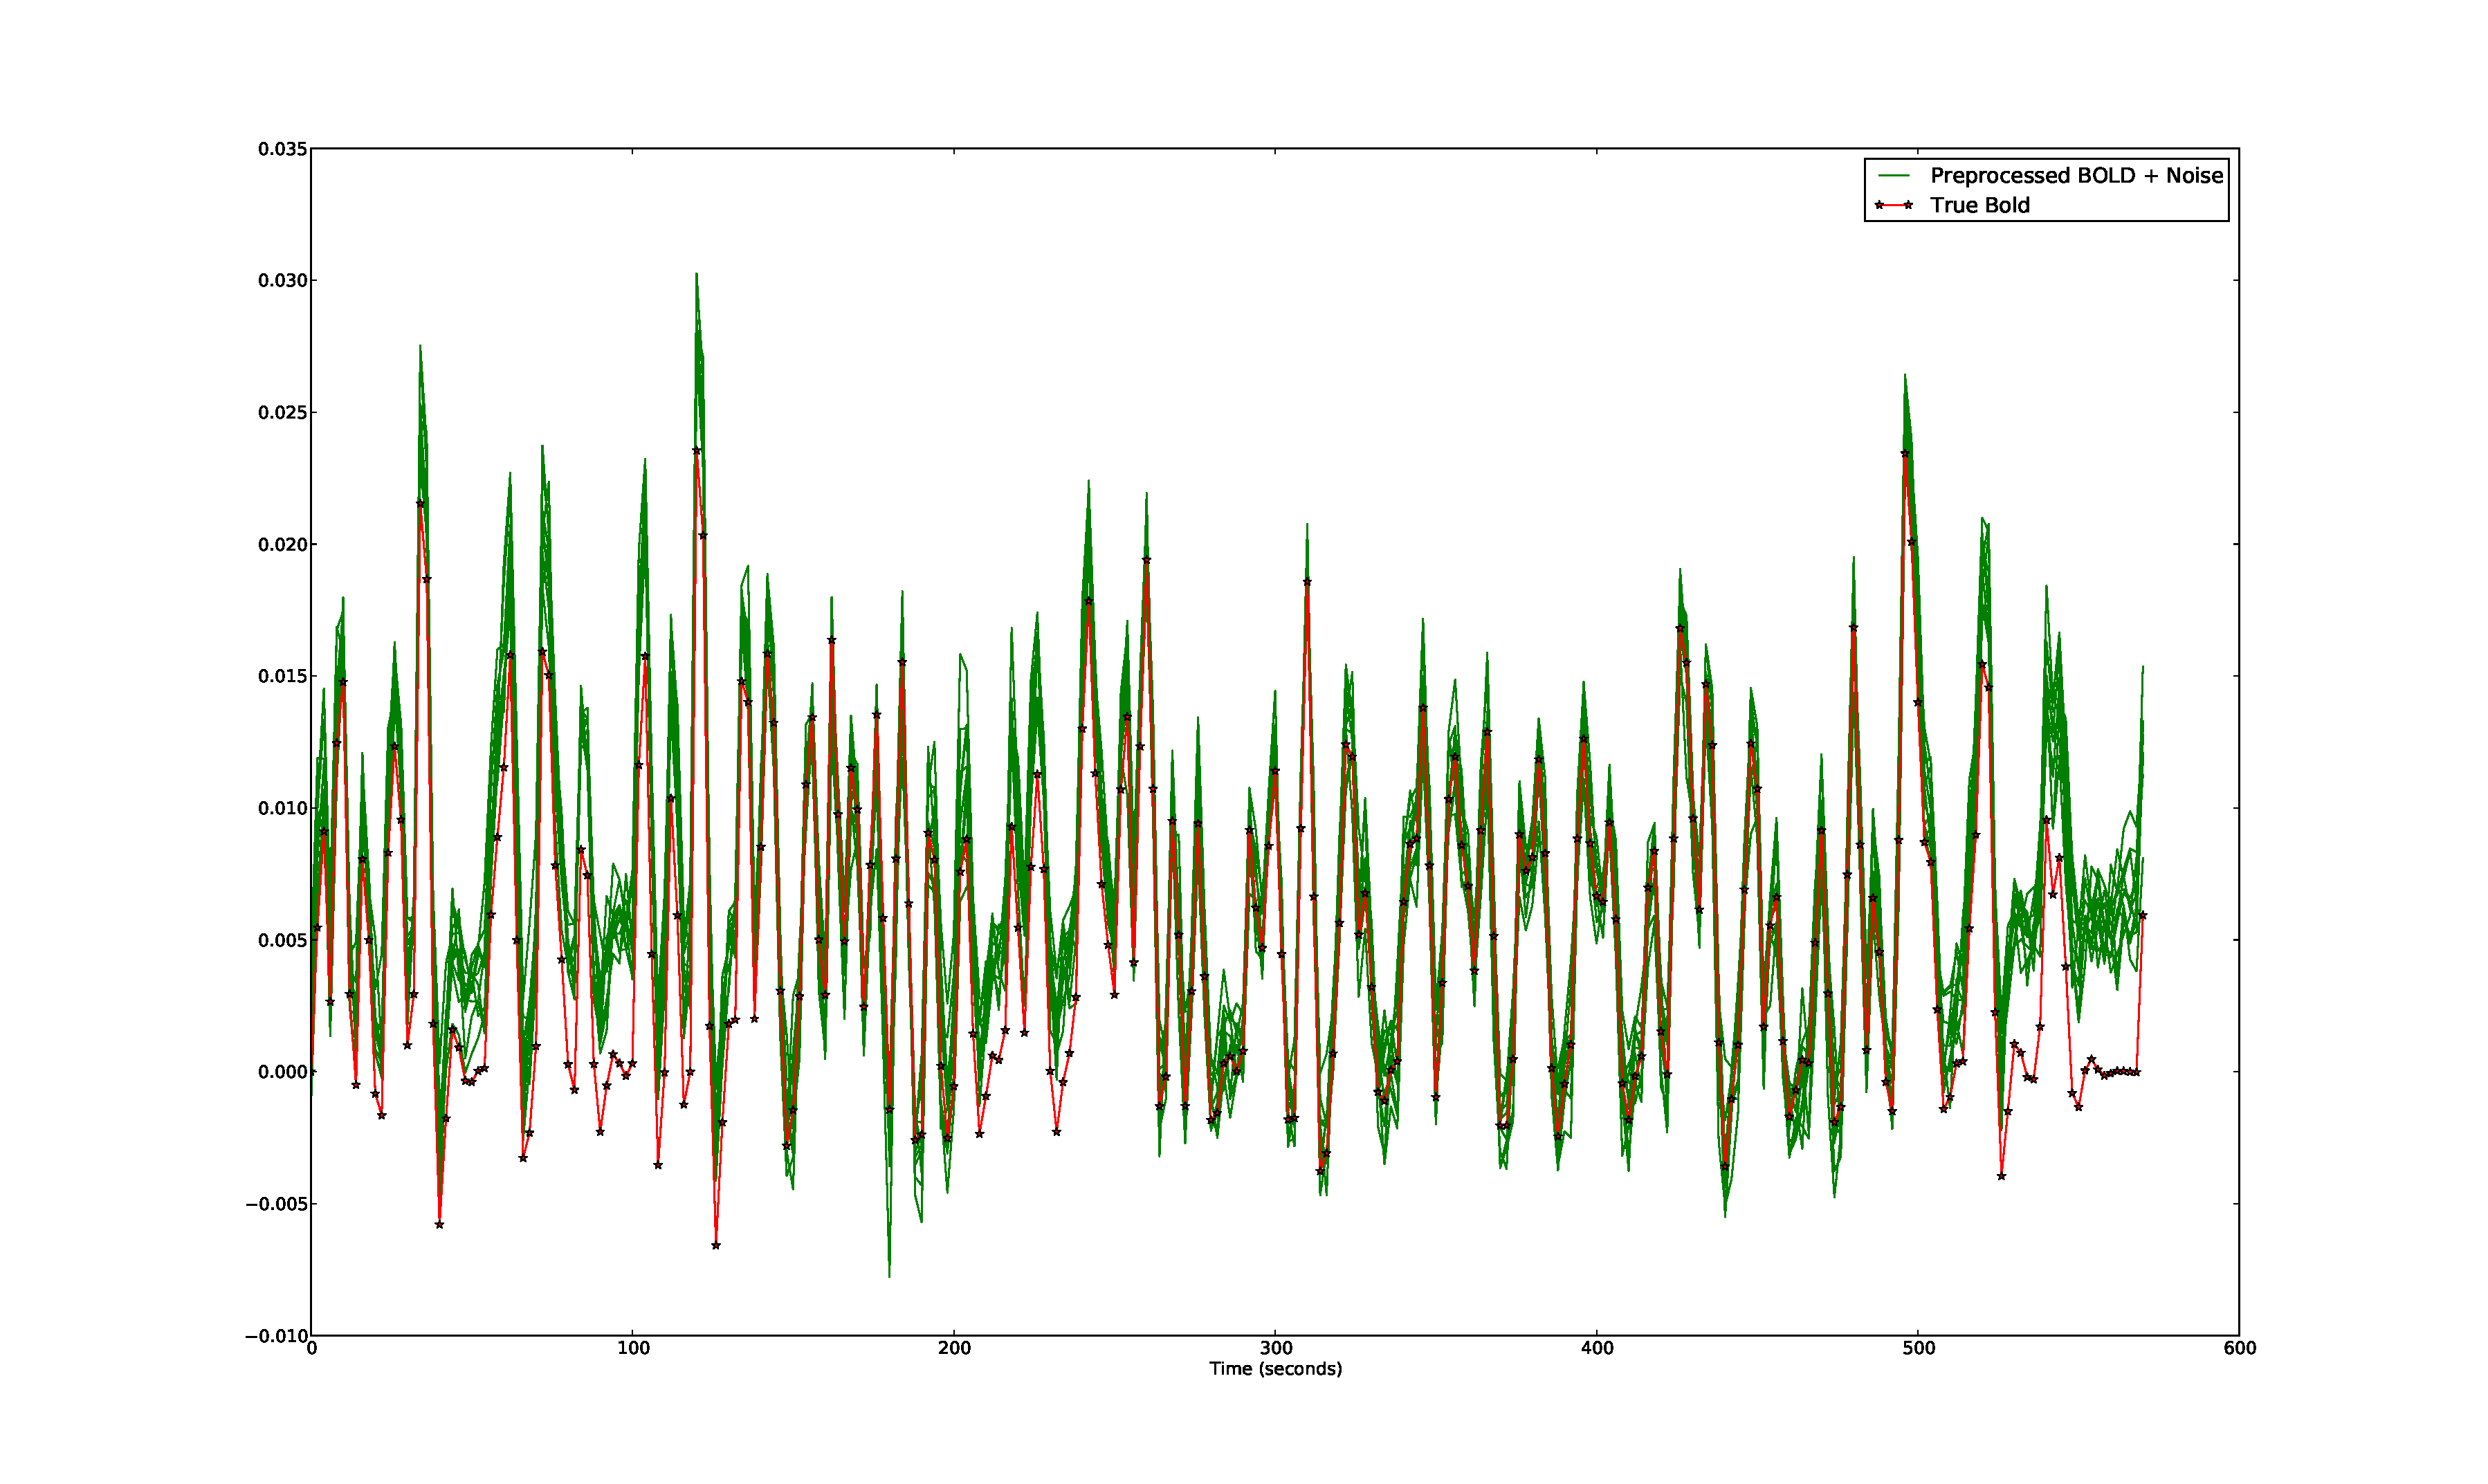
\includegraphics[clip=true,trim=6cm 2cm 5cm 3.5cm,width=15cm]{images/preprocessed_lownoise}
\caption{A comparison of the preprocessed signals for the low noise case. The
noisy input to the actual particle filter algorithm.}
\label{fig:PreprocessedLowNoise}
\end{figure}

\begin{figure}
\centering
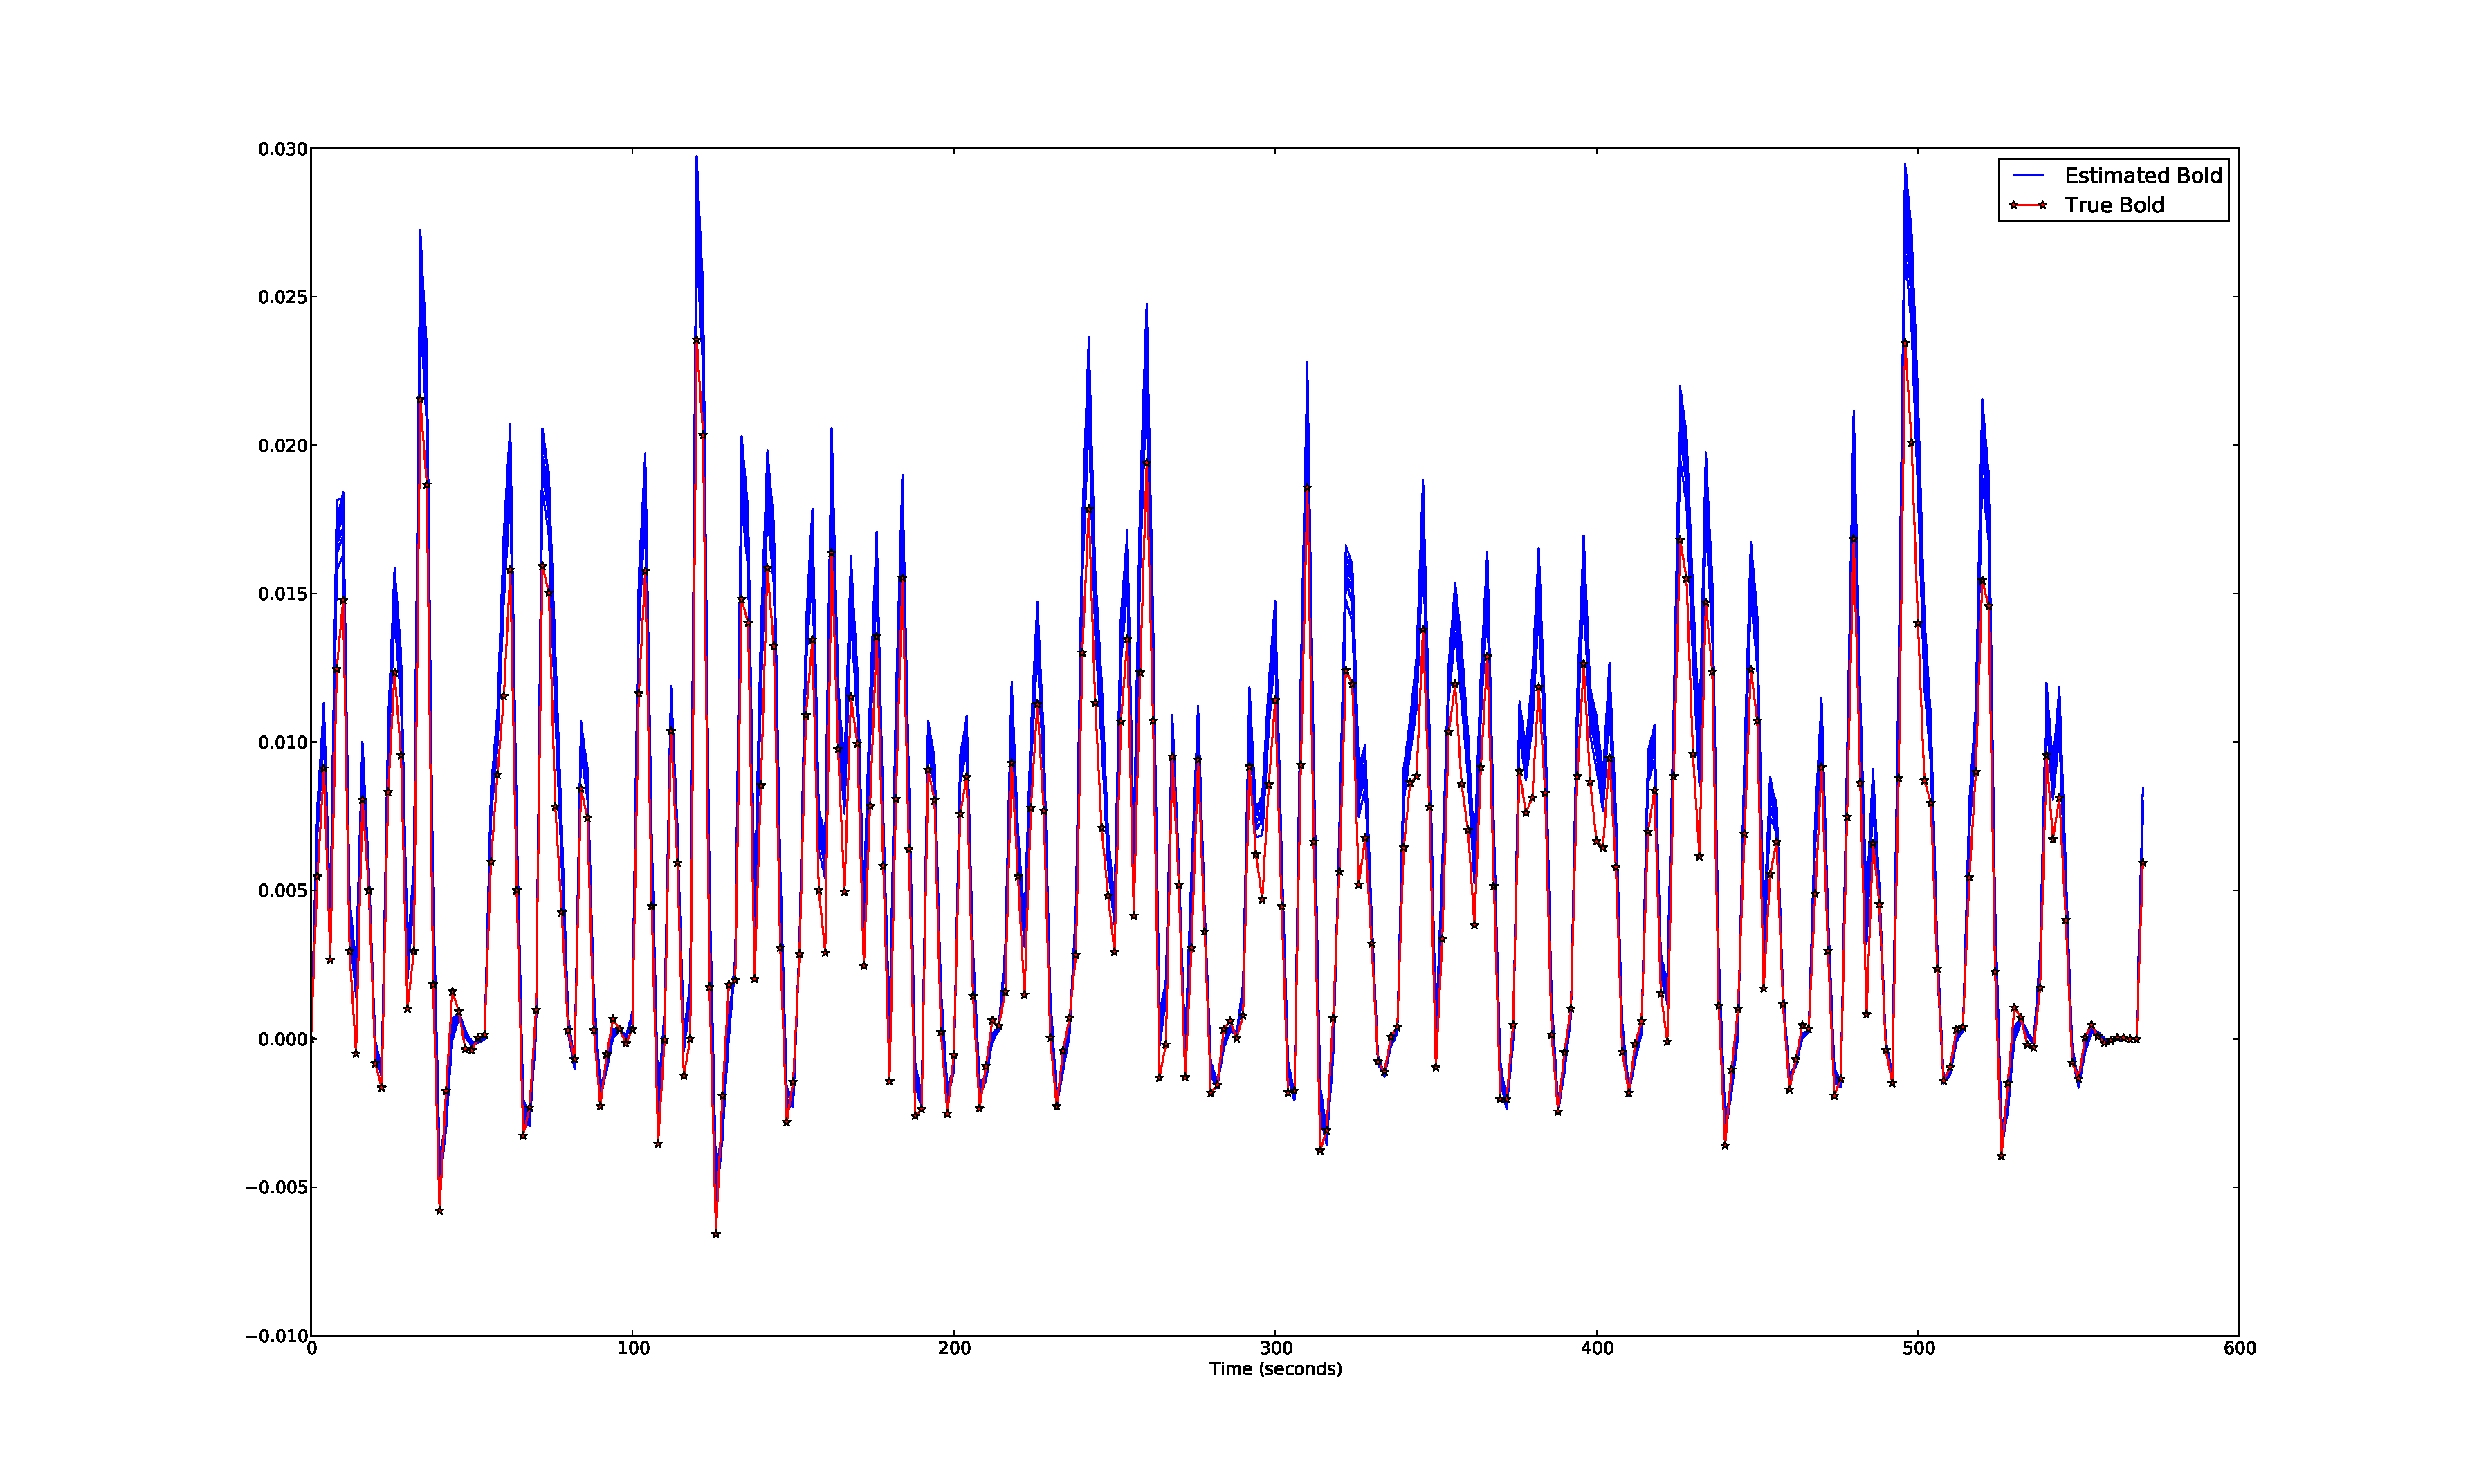
\includegraphics[clip=true,trim=6cm 2cm 5cm 3.5cm,width=15cm]{images/comparison_lownoise}
\caption{A comparison of the fitted signals for the low noise case.}
\label{fig:FitComparisonLowNoise}
\end{figure}

\begin{table}[t]
\centering
\begin{tabular}{|c | c | c | c | c | c | c | c | c | c |}
\hline 
$\tau_0$ & $\alpha$ & $E_0$    & $V_0$    & $\tau_s$ & $\tau_f$ & $\epsilon$  & $ \sum \tau $ & Residual & Error\\
\hline 
\rowcolor[gray]{.8}
1.45 & 0.3 & 0.47 & 0.044 & 1.94 & 1.99 & 1.8  & 5.38 &  & \\
\hline 
\hline 
1.2221 & 0.3449 & 0.3346 & 0.0714 & 1.6045 & 2.2753 & 1.5945 & 5.1019 &  0.003211  & 0.009876  \\
1.3749 & 0.3318 & 0.3630 & 0.0733 & 1.6408 & 2.1030 & 1.5763 & 5.1187 &  0.003055  & 0.009932  \\
1.1660 & 0.3221 & 0.3406 & 0.0822 & 1.6477 & 2.3535 & 1.2452 & 5.1672 &  0.003289  & 0.009680  \\
1.2318 & 0.3271 & 0.3403 & 0.0796 & 1.6270 & 2.1852 & 1.3033 & 5.0439 &  0.002847  & 0.009120  \\
1.1832 & 0.3179 & 0.3472 & 0.0821 & 1.5496 & 2.2912 & 1.2782 & 5.0240 &  0.003006  & 0.009713  \\
1.1424 & 0.334  & 0.3473 & 0.0737 & 1.6221 & 2.2908 & 1.4025 & 5.0553 &  0.002833  & 0.009485  \\
1.3004 & 0.3596 & 0.3564 & 0.0768 & 1.5641 & 2.1323 & 1.6034 & 4.9968 &  0.003028  & 0.010219  \\
1.2401 & 0.3460 & 0.3398 & 0.0891 & 1.6499 & 2.2366 & 1.2900 & 5.1265 &  0.003044  & 0.010080  \\
1.1709 & 0.3274 & 0.3464 & 0.0826 & 1.5373 & 2.2826 & 1.3783 & 4.9909 &  0.003345  & 0.010329  \\
1.1897 & 0.3434 & 0.3355 & 0.0798 & 1.5358 & 2.3075 & 1.4277 & 5.0330 &  0.003175  & 0.010015  \\
1.184 &  0.3405 & 0.3502 & 0.0892 & 1.6103 & 2.2793 & 1.1645 & 5.0735 &  0.002889  & 0.009505  \\
\hline                                                                           
1.2187 & 0.3359 & 0.3456 & 0.0800 & 1.599 & 2.2488 & 1.3876 & 5.0665 & 0.003066     & 0.009814 \\
\hline 
\end{tabular}
\caption{Estimated Parameters on 11 different runs with low noise. First row is the true value, and last is the average.}
\label{tab:LowNoiseResults} 
\end{table}

\begin{figure}
\subfigure[Converging histogram for $\tau_0$, $\alpha$, $E_0$, and $V_0$ of the first run, low noise simulation.]
{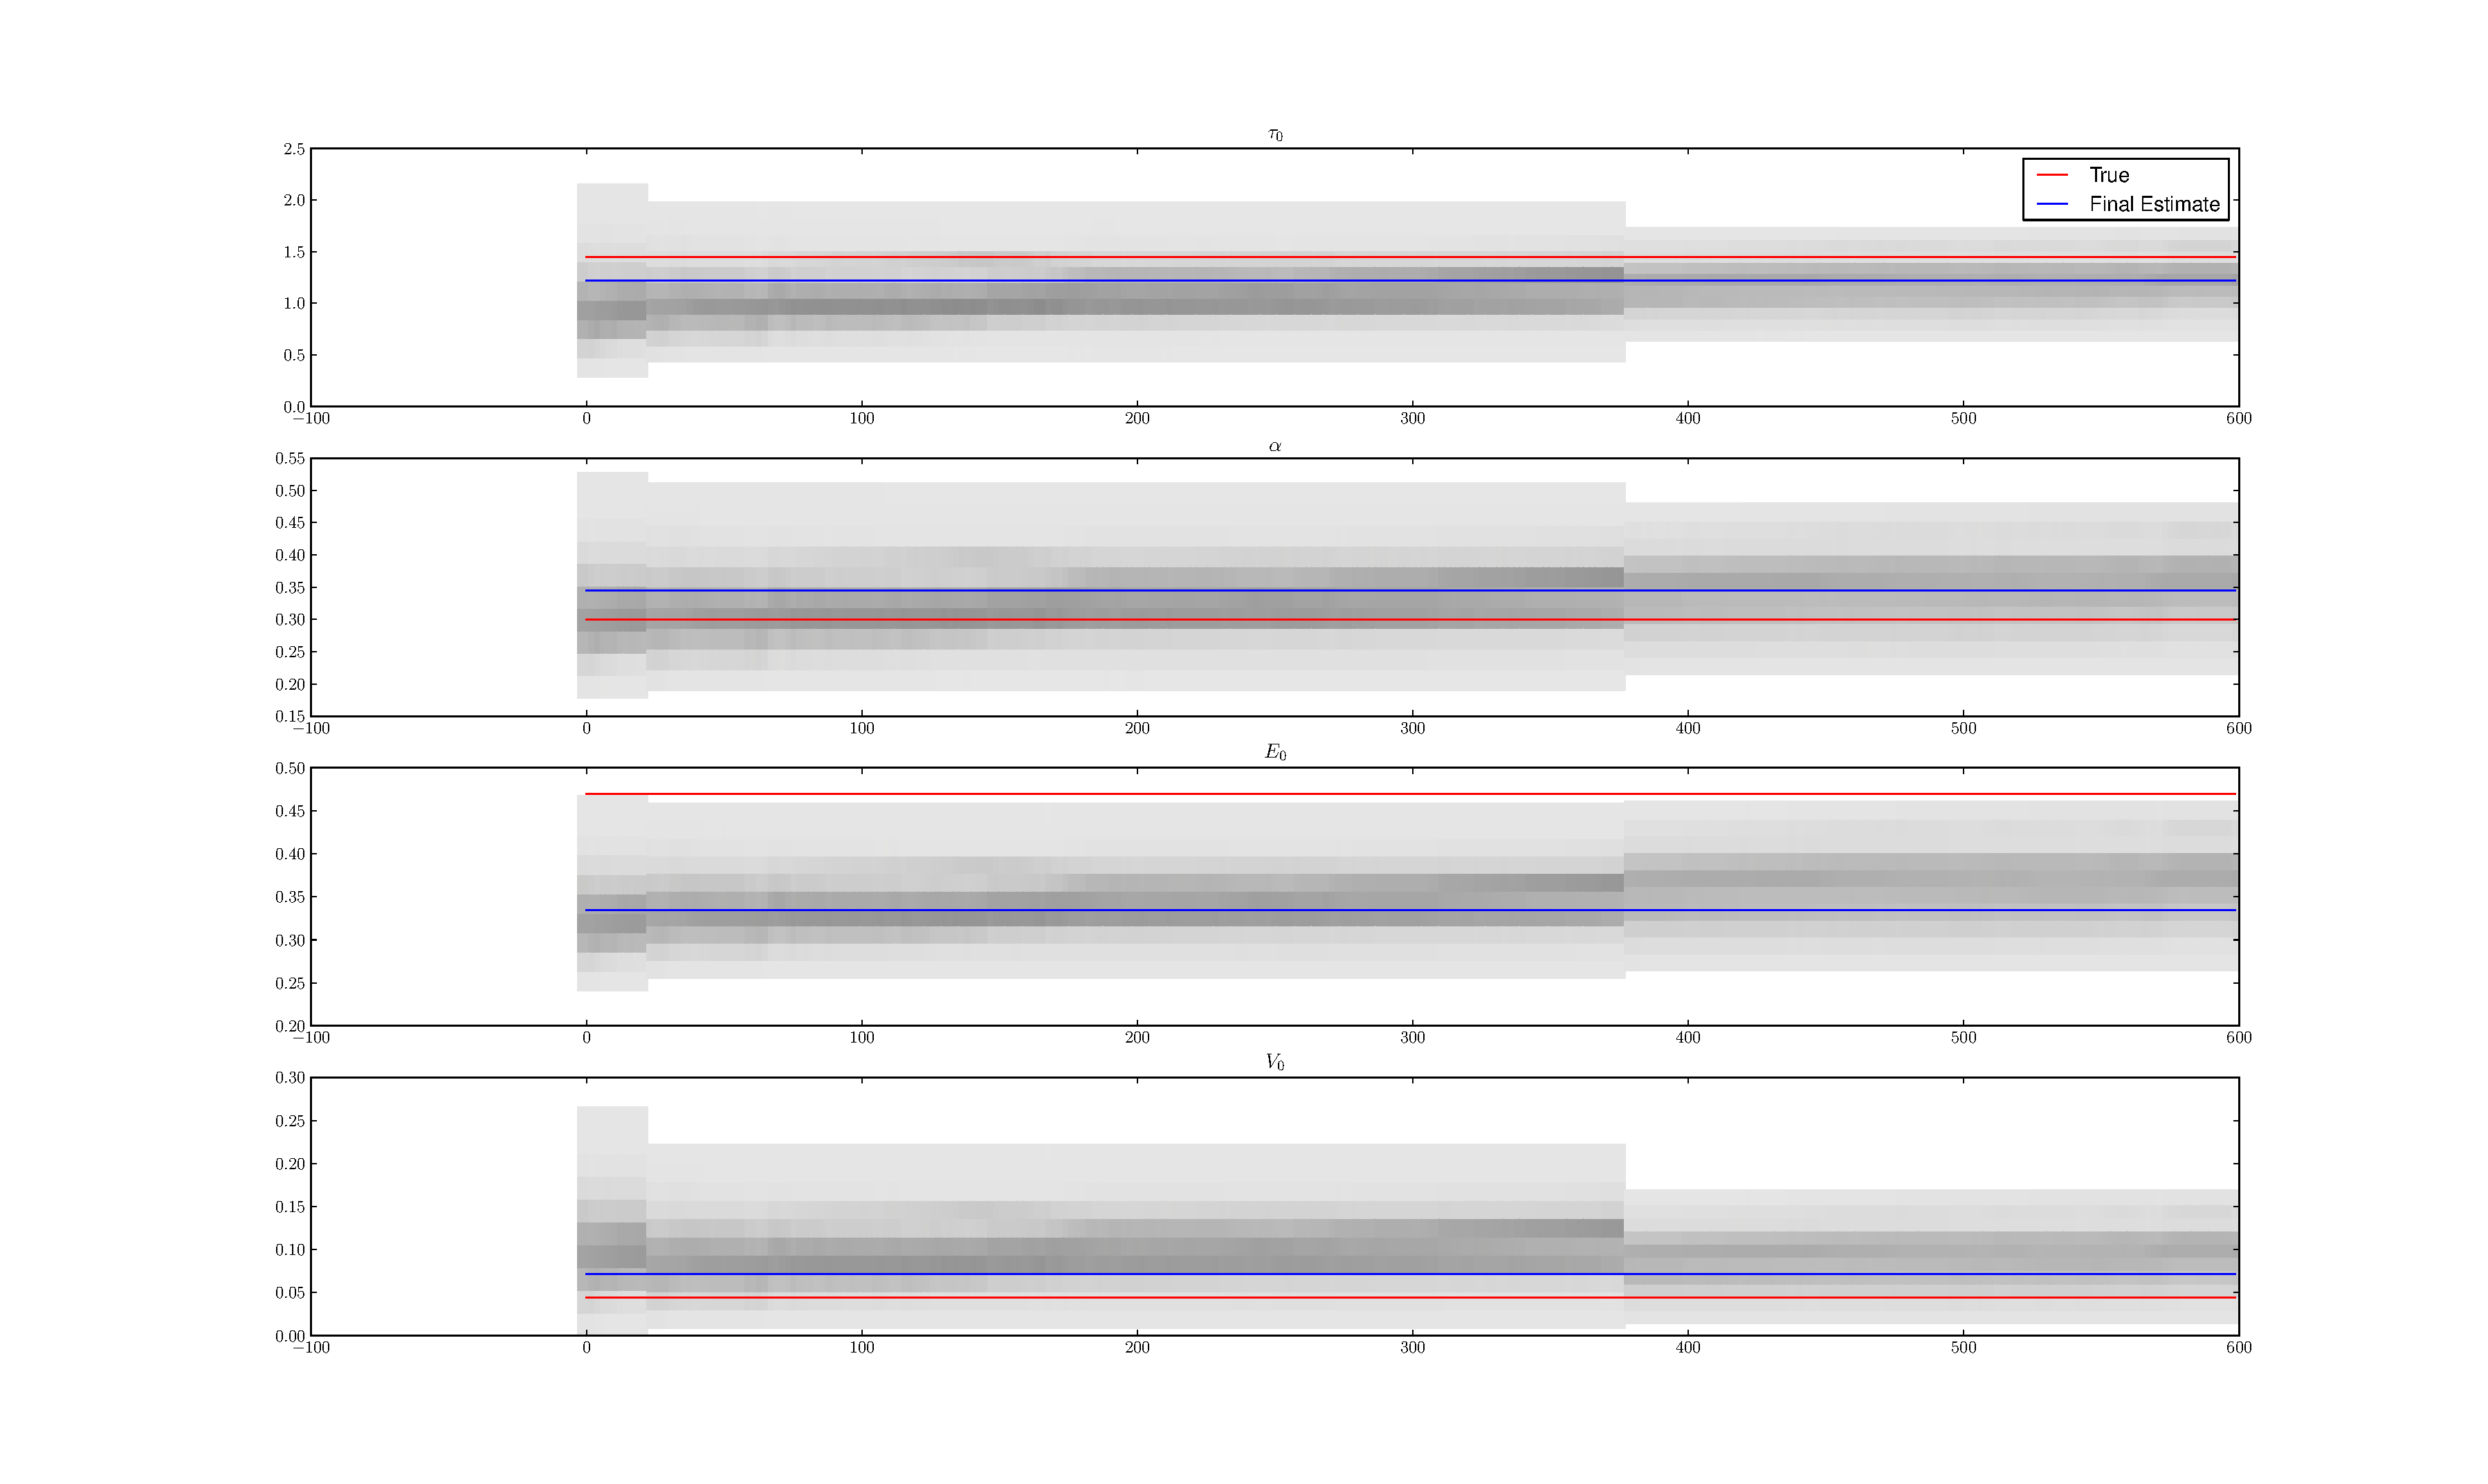
\includegraphics[clip=true,trim=7cm 3cm 6cm 3cm, width=16cm]{images/converge_lownoise1}}\\

\subfigure[Converging histogram for $\tau_s$, $\tau_f$, $\epsilon$, and $v$ of the first run, low noise simulation.]
{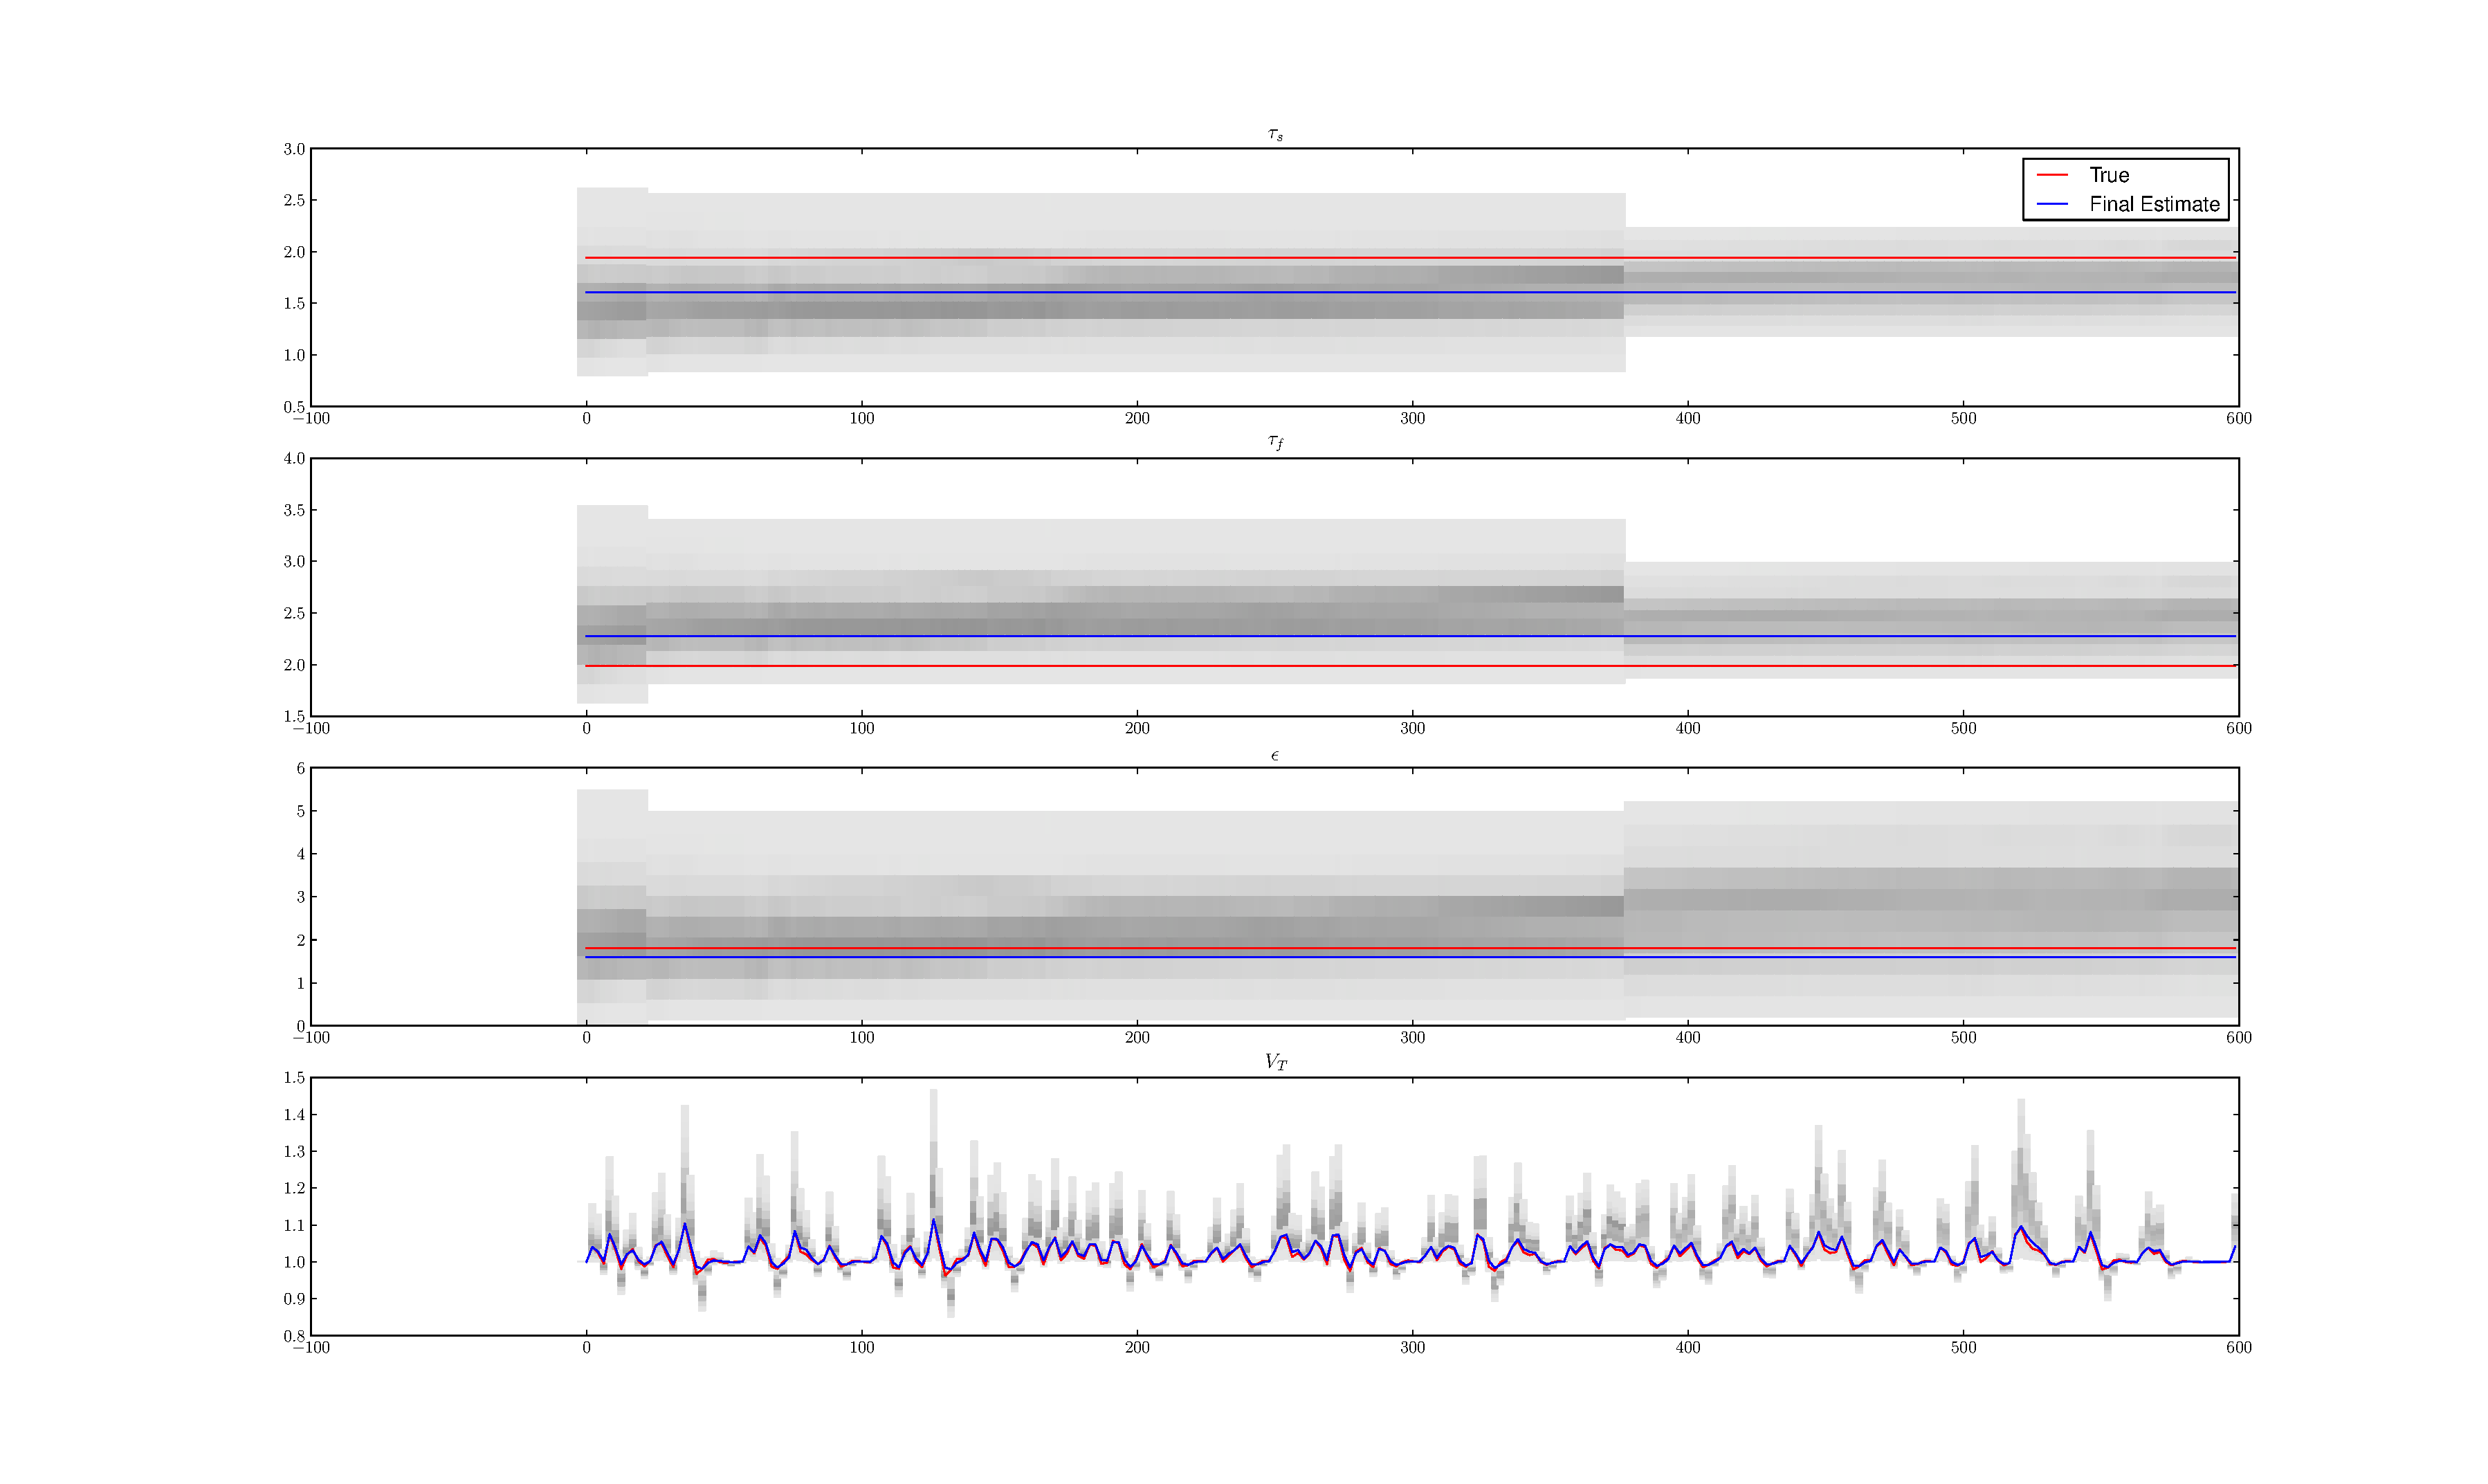
\includegraphics[clip=true,trim=7cm 3cm 6cm 3cm, width=16cm]{images/converge_lownoise2}}\\
\end{figure}

\begin{figure}
\subfigure[Converging histogram for $q$, $s$, $f$, and $BOLD$ of the first run, low noise simulation.]
{\label{fig:LowNoiseHistc} 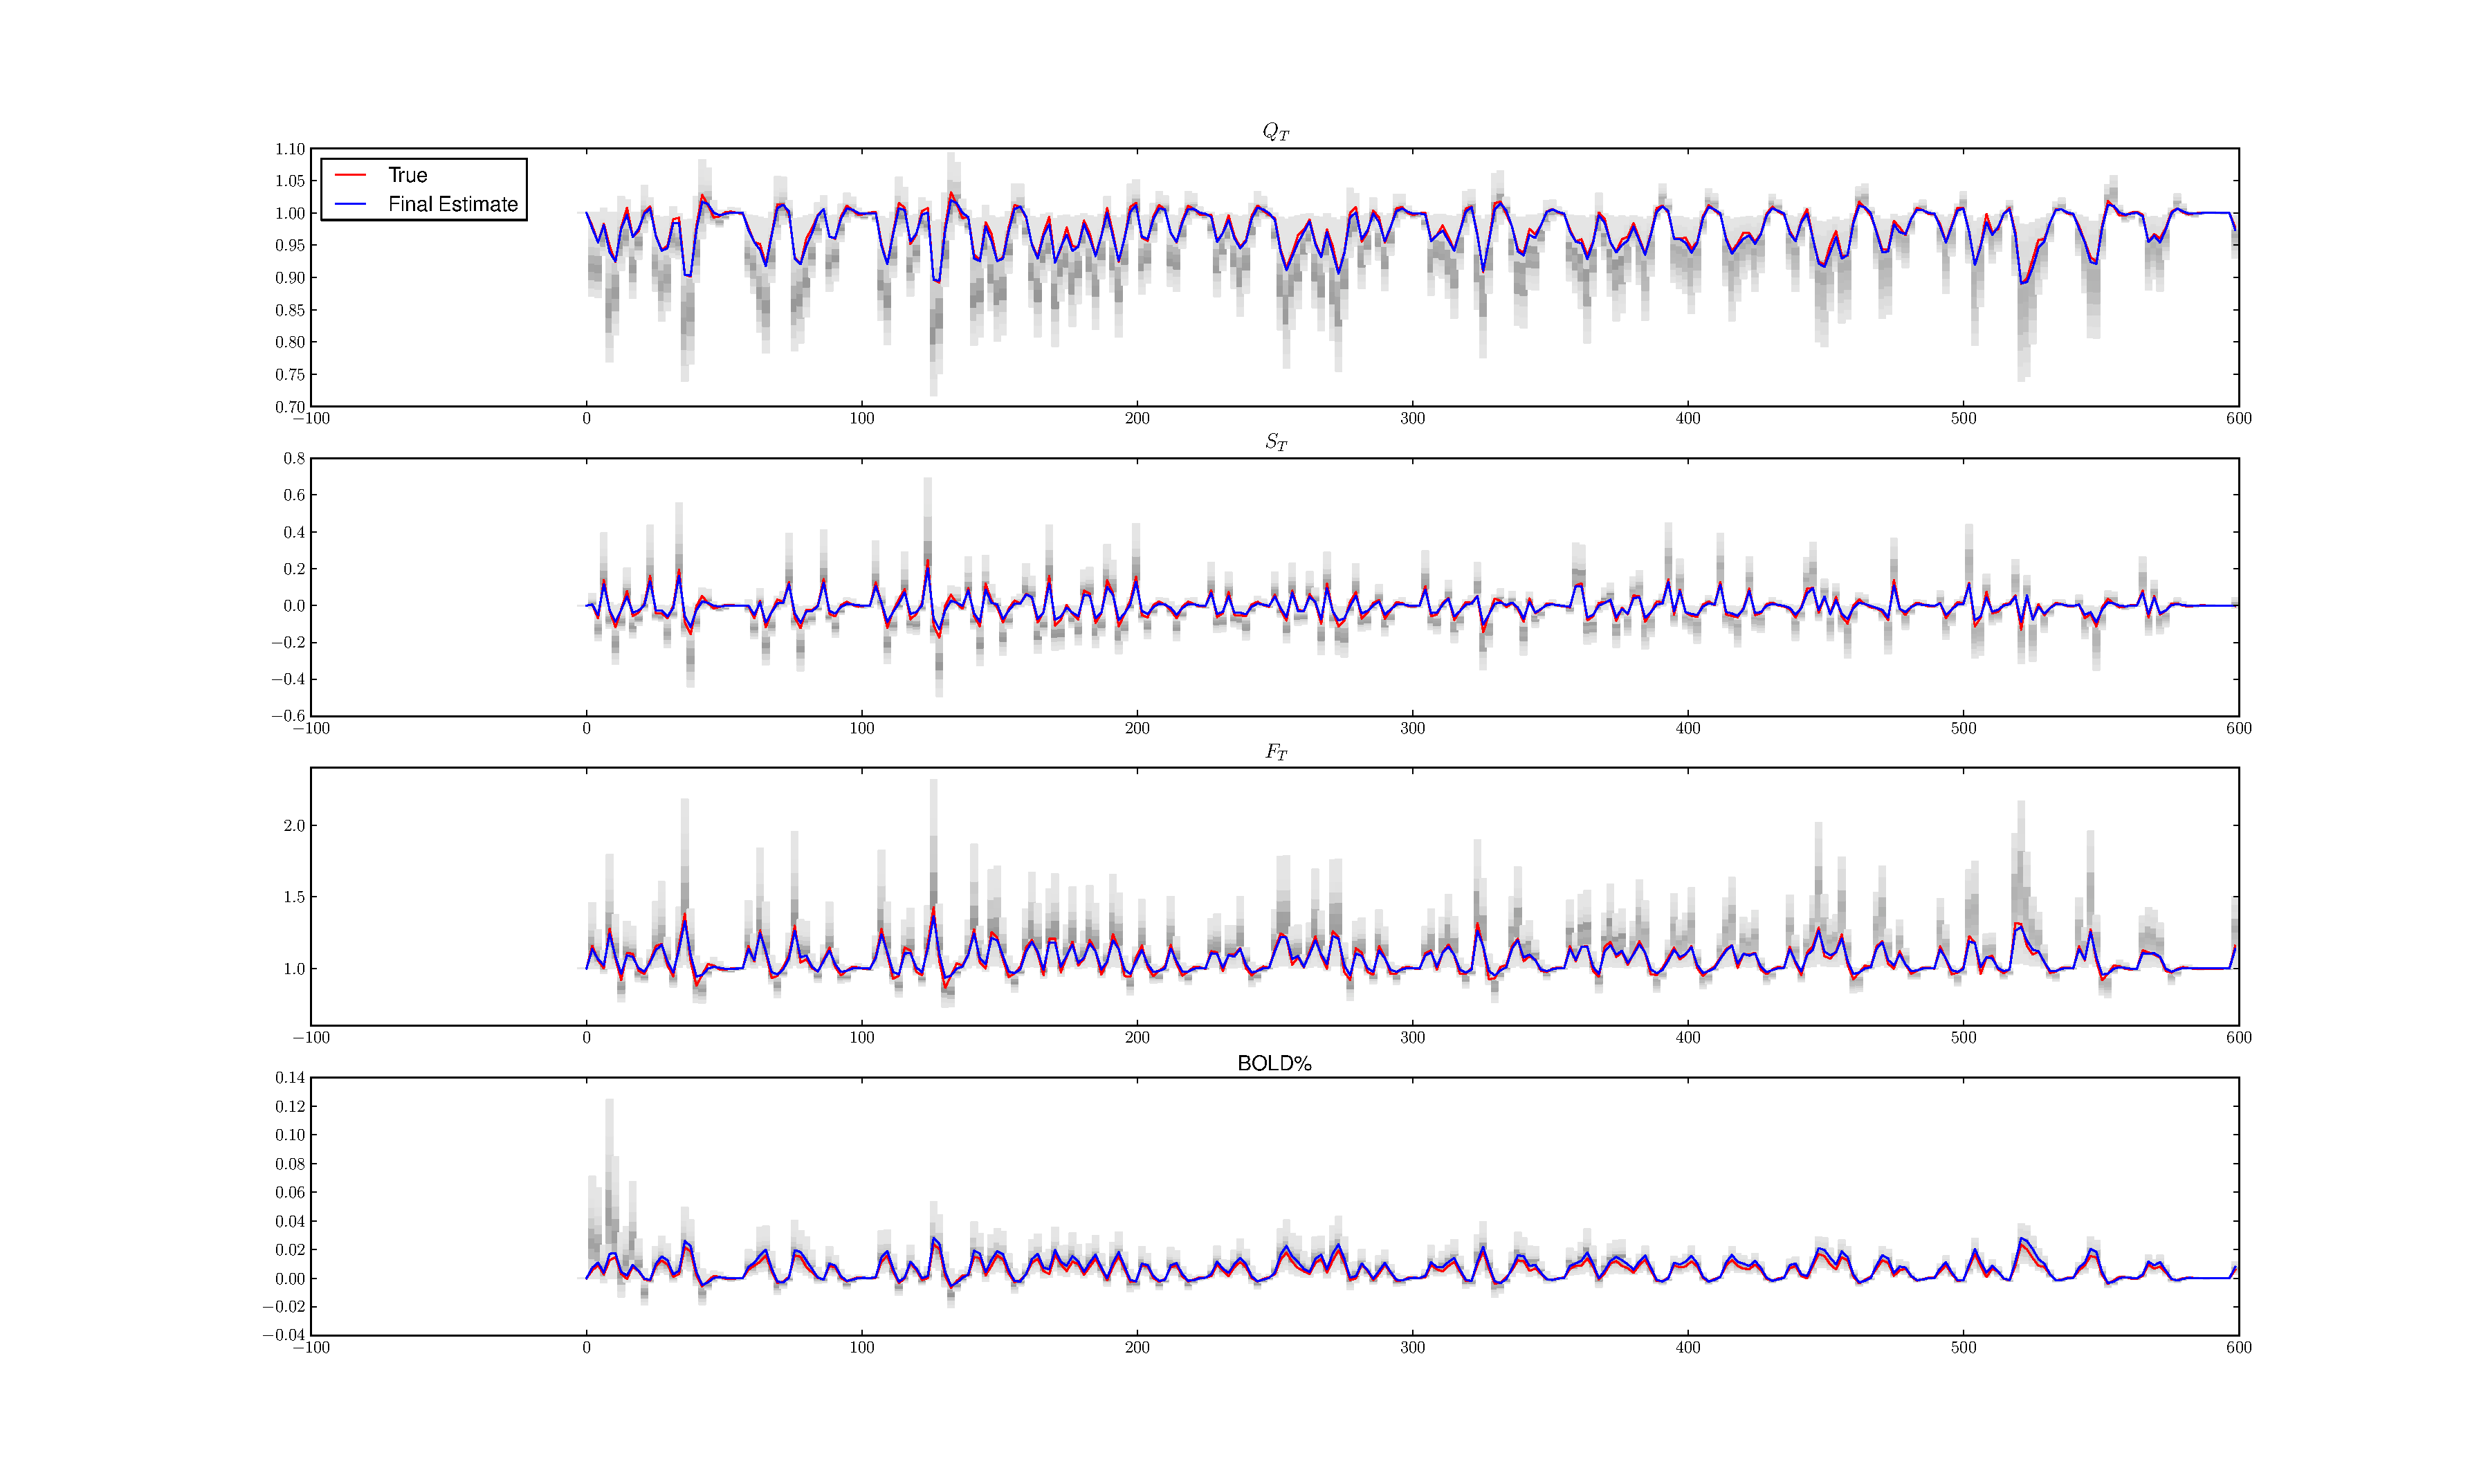
\includegraphics[clip=true,trim=7cm 3cm 6cm 3cm, width=16cm]{images/converge_lownoise3}}
\caption{Convergence of the first run from \autoref{tab:LowNoiseResults}. The bars represent
a histogram, where darker bars indicate more particles in that bin.}
\label{fig:LowNoiseHist}
\end{figure}

The following tests all use less data (shorter sequences), on par with 
the average length of an FMRI session. For this low noise case 
$(\sigma_y = 0.001,\ \sigma_x = .0005)$, the eleven realizations are shown in 
\autoref{fig:LowNoiseRealization}.
The bias introduced into the signal by preprocessing 
could have some effect on the resulting fit; thus the preprocessed signal is compared
to the true BOLD signal in \autoref{fig:PreprocessedLowNoise}.
Overall, \autoref{fig:PreprocessedLowNoise} shows that the preprocessing was 
effective at removing trends, although the spline did struggle to match the signal 
torward the end. This slight drift effect was caused by the final median being 
well above the base
level. 
At several time points the particle filter successfully filtered the input
(\autoref{fig:FitComparisonLowNoise}).
For instance, in the last 30 seconds
the estimates stay flat in spite of the preprocessed data drifting off. By
this point, the algorithm had converged sufficiently to prevent such inexplicable movement.
A similar circumstance occurs at around 100 seconds in. A combination of 
noise and preprocessing biased the results toward a peak signal above the true peaks. 
The final parameter sets are shown in 
\autoref{tab:LowNoiseResults}. 


Note that throughout the results, unless otherwise specified,
the term \emph{residual} will be defined as the square root of the mean squared residual, 
\begin{equation}
\text{Residual} = \sqrt{\sum (\hat{y}_k - y_k)^2}
\end{equation}
where $\hat{y}_k$ is the estimated output at time $k$ and $y_k$ is the preprocessed output
sampled at time $k$. Note the subtle distinction between this and what will be 
termed the \emph{error} which is defines as 
\begin{equation}
\text{Error} = \sqrt{\sum (\hat{y}_k - Y_k)^2}
\end{equation}
where $\hat{y}_k$ is the estimated output, and $Y_k$ is the underlying (free of noise)
signal. Throughout this section and the next, the terms error and residual
will be referencing these values.

%\begin{table}[t]
%\centering
%\begin{tabular}{|c | c  c  c  c  c  c  c |}
%\hline 
%  & $\tau_0$ & $\alpha$ & $E_0$    & $V_0$    & $\tau_s$ & $\tau_f$ & $\epsilon$ \\
%\hline 
%\rowcolor[gray]{.8} $\tau_0$ &   0.0189481 & -0.0014269 & -0.0011267 & -1.13e-05 & -0.0025616 & -0.0189559 & 0.0070405 \\
%$\alpha$ &                       -0.0014269 & 0.0026716 & 9.93e-05 & -0.0002041 & -0.0008632 & -0.0016823 & 0.0071891 \\
%\rowcolor[gray]{.8} $E_0$    &   -0.0011267 & 9.93e-05 & 0.0010701 & -0.0002277 & -0.0001177 & 0.0001013 & 0.0016972 \\
%$V_0$    &                       -1.13e-05 & -0.0002041 & -0.0002277 & 0.0005401 & 4.3e-06 & 4.56e-05 & -0.0080494 \\
%\rowcolor[gray]{.8} $\tau_s$ &   -0.0025616 & -0.0008632 & -0.0001177 & 4.3e-06 & 0.0128056 & 0.012878 & -0.005516 \\
%$\tau_f$ &                       -0.0189559 & -0.0016823 & 0.0001013 & 4.56e-05 & 0.012878 & 0.0416927 & -0.0158182 \\
%\rowcolor[gray]{.8} $\epsilon$&  0.0070405 & 0.0071891 & 0.0016972 & -0.0080494 & -0.005516 & -0.0158182 & 0.1567165 \\
%\hline 
%\end{tabular}
%\caption{Typical Covariance matrix of the parameters at the end of a run.}
%\label{tab:CovSim} 
%\end{table}

There are a few important results in the final parameter estimates (which 
are the mean of the particle filter's posterior distribution). First, the time constants vary 
greatly across
runs, yet the sum of the individual time constants
($\tau_f$, $\tau_s$ and $\tau_0$) were more consistent. In general the 
time constants fell short of the true time constant. This could be a limitation
based on the prior distribution (which notably has an initial mean below the true values) 
or it could be that other parameters compensated. It is also possible that the output is insensitive
to small differences in the time constants.  
The convergence properties of the first run in \autoref{tab:LowNoiseResults} 
demonstrates the migration of parameters through the run. In spite of the
significant differences in parameter estimates, the estimated BOLD
consistently performed well 
(\autoref{fig:FitComparisonLowNoise}).


%The large variation of $V_0$ are also interesting, although as the final
%covariance matrix of the first run shows, there is a significant correlation between $\epsilon$ and $V_0$.
%In general, with even a small amount of noise, parameters are ill defined. Thus at
%least for this set of stimuli the parameters are not uniquely identifiable. 
%
%The covariance matrix (\autoref{tab:CovSim}) provides a great deal of insight into 
%the way parameters evolve in the particle filter. The number of 
%covariance elements that exceed the variance elements indicates the
%significant interplay between parameters. Every single parameters, including $\alpha$, 
%has a non-zero covariance. Why $\alpha$ and $\epsilon$ would be positively related
%is the most interesting element. The answer of how exactly each parameter
%compensates for other parameters is complex.  Notice the covariance of $\tau_f$ and $\tau_0$
%is $-0.019$ whereas the variance of $\tau_0$ and $\tau_f$ are $0.019$ and $0.04$ respectively. 
%%stopped here
%As Clearly there is some measure of ill-defined behavior between the different time-constants, which is to
%be expected given the number steps before a stimuli affects the output. 
%The convergence properties of the first run in \autoref{tab:LowNoiseResults} 
%demonstrates the migration of parameters to match the estimates. Given the relatively high
%variance of parameters, its likely that more measurements or perhaps more variation
%in the stimuli could further differentiate the parameters. Its also notable that
%the final mean of the parameters may not be the best point estimator, and that perhaps
%using the mode would be a better way to estimate the output. Regardless, the time series'
%generated from the estimated mean seems to match the correct signal very well 
%(\autoref{fig:FitComparisonLowNoise}).

%HIGH NOISE SECTION, with a signal
\subsection{Simulation with High Noise}
\label{sec:SimHighNoise}
%\begin{figure}
%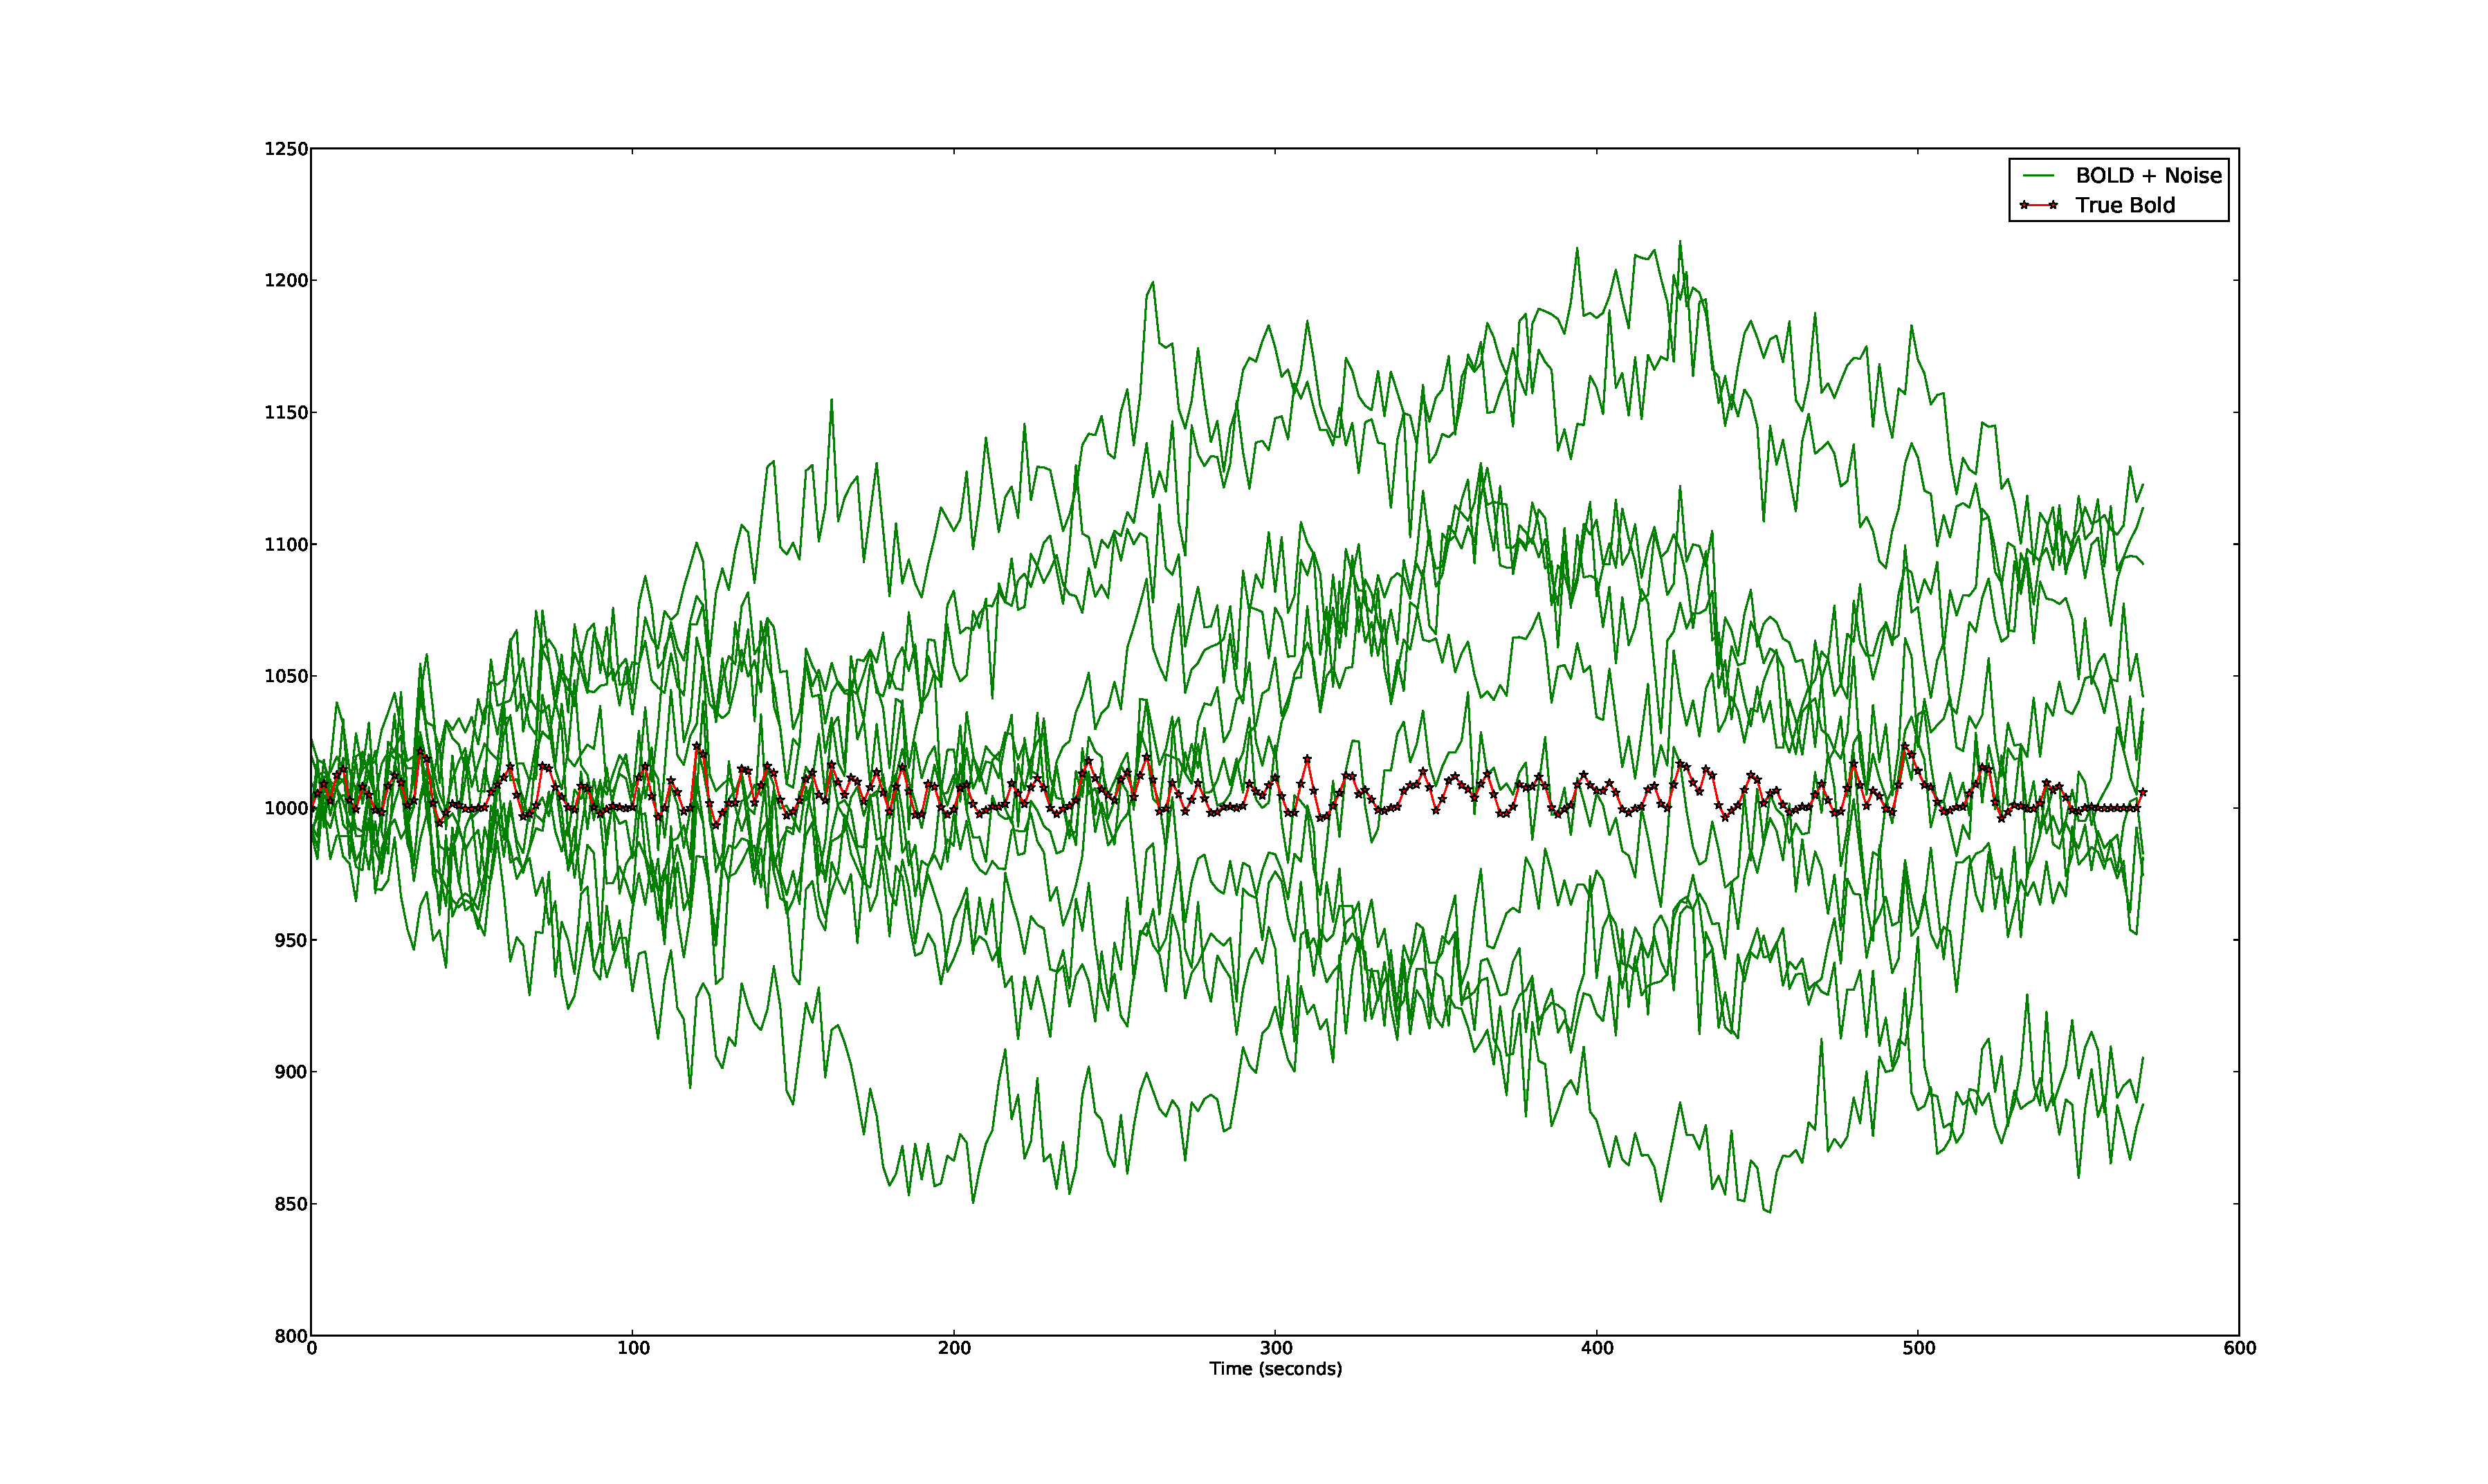
\includegraphics[clip=true,trim=6cm 2cm 5cm 3.5cm,width=15cm]{images/realization_highnoise}
%\caption{Test Signals with high noise ($\sigma_x = 0.01, \sigma_y=0.005$) compared to the clean signal.}
%\label{fig:HighNoiseRealization}
%\end{figure}

\begin{figure}
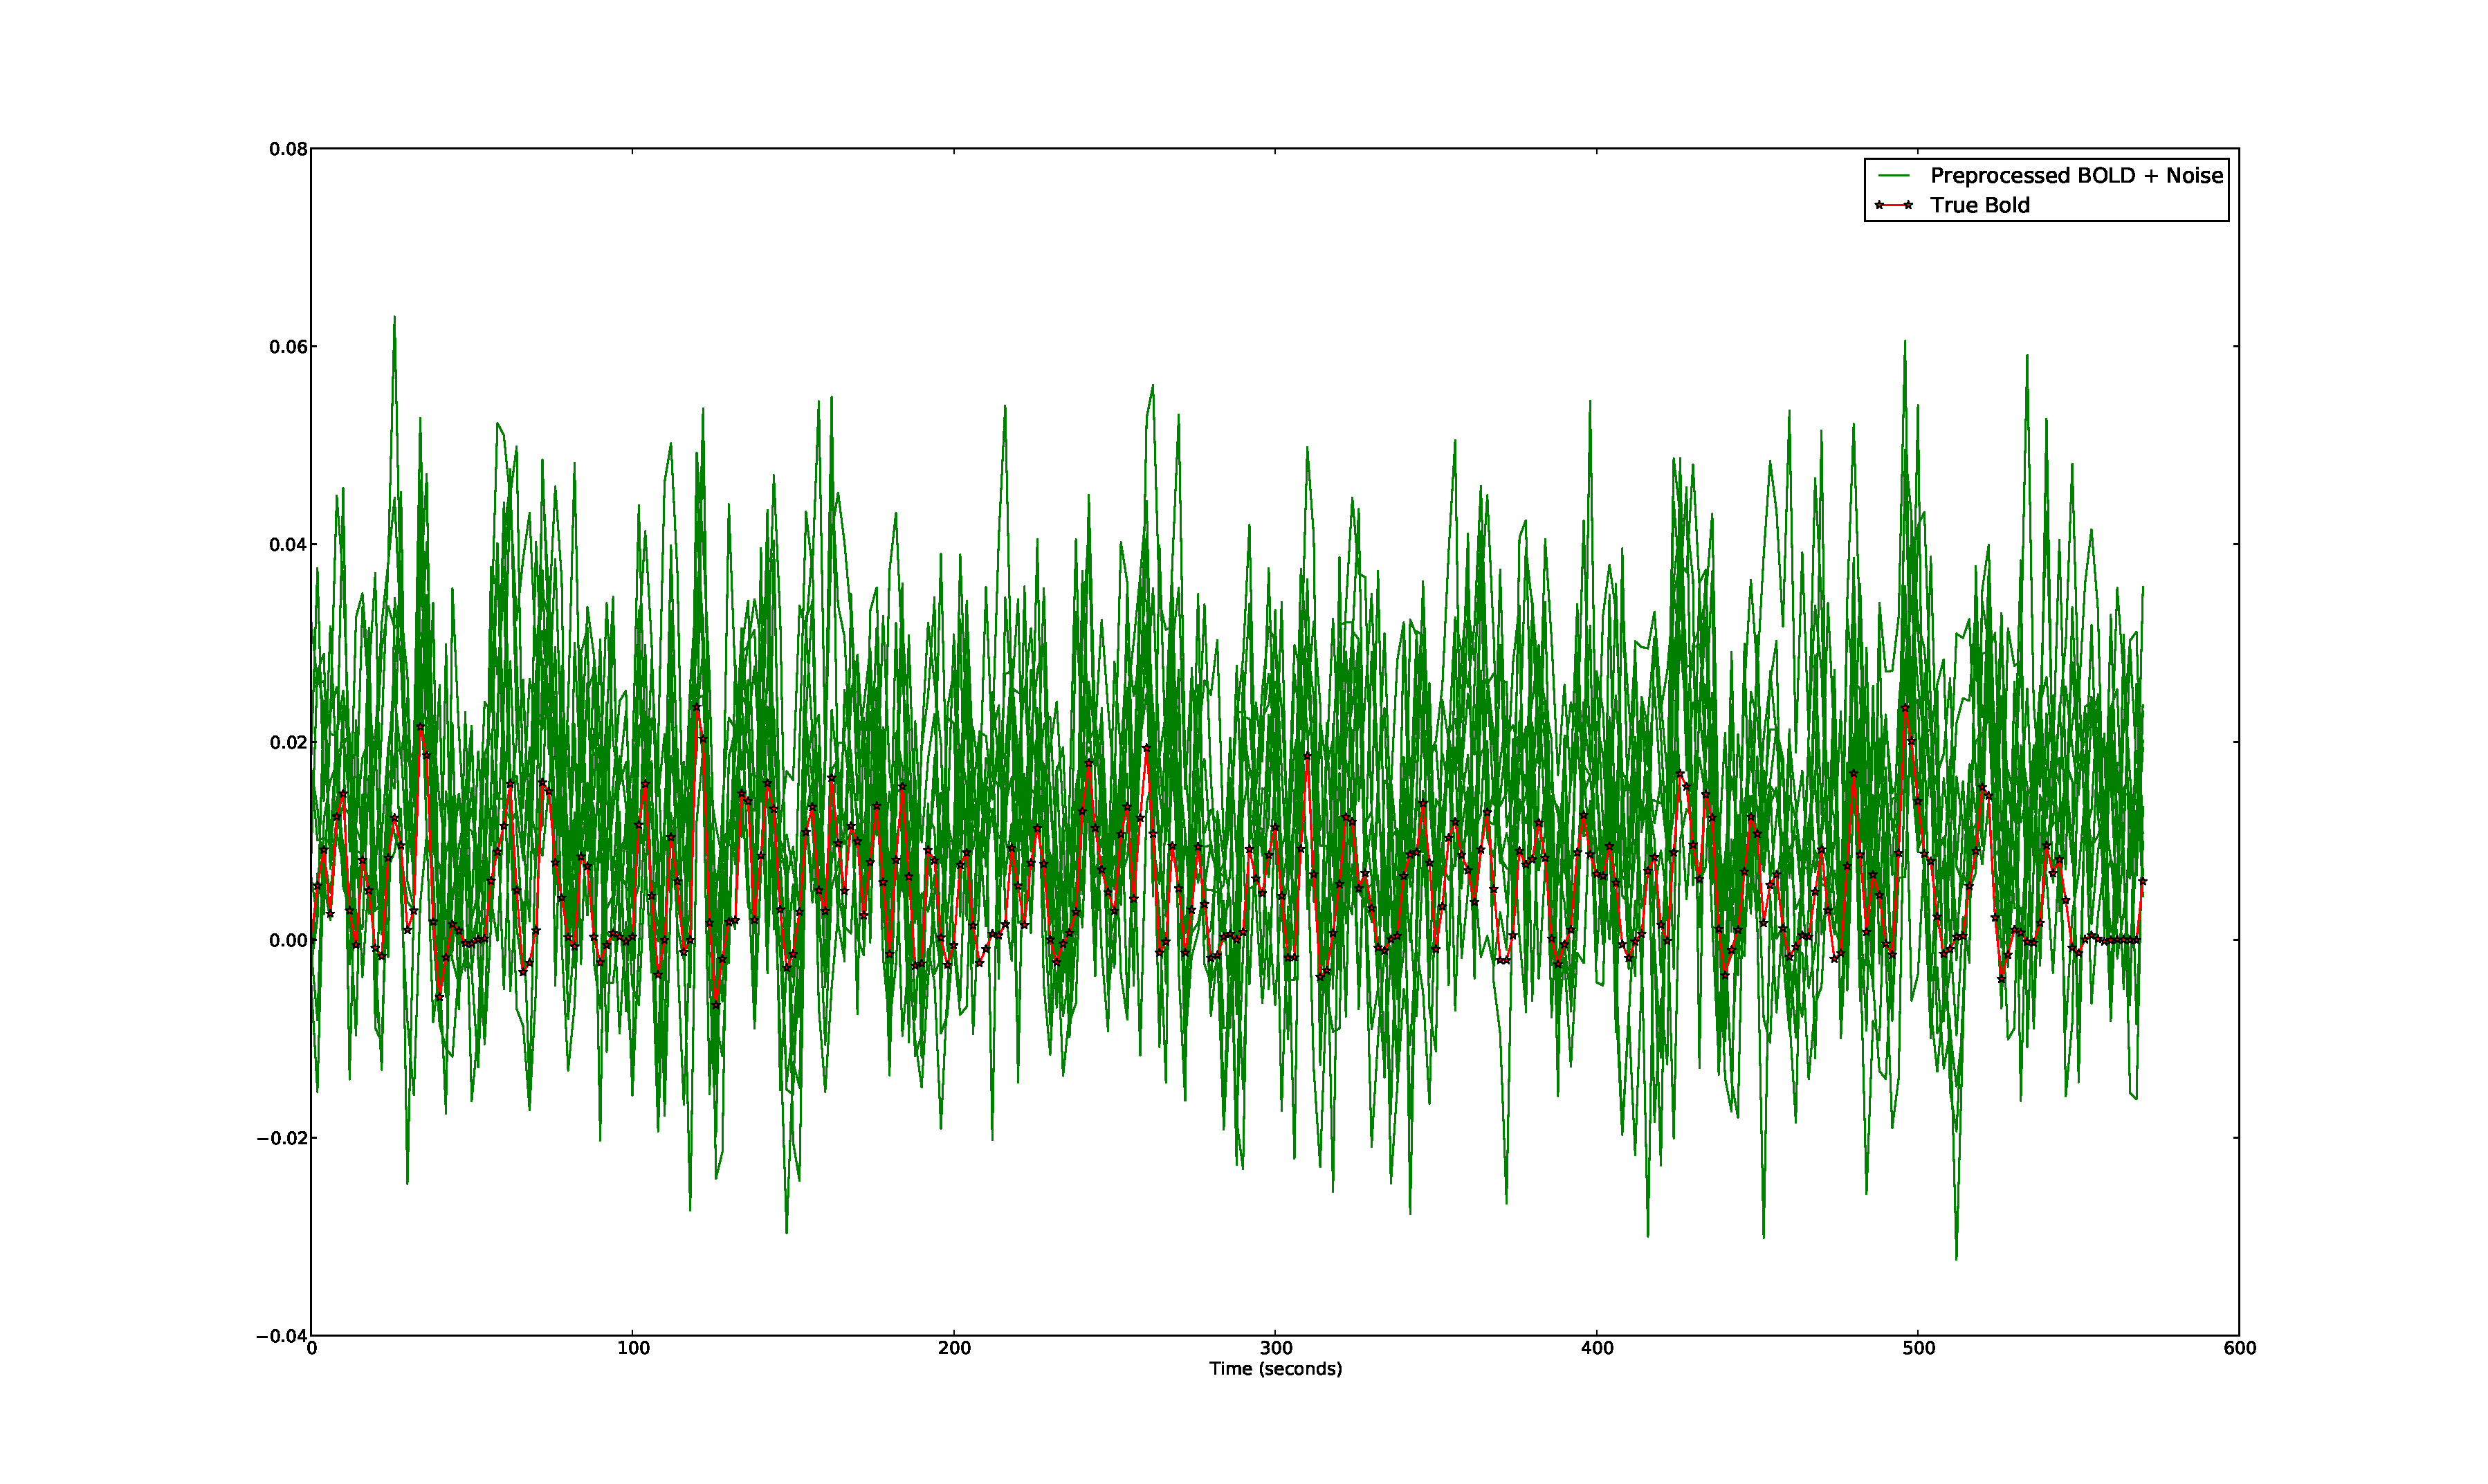
\includegraphics[clip=true,trim=6cm 2cm 5cm 3.5cm,width=15cm]{images/preprocessed_highnoise}
\caption{A comparison of the preprocessed signals for the high noise case.}
\label{fig:PreprocessedHighNoise}
\end{figure}

\begin{figure}
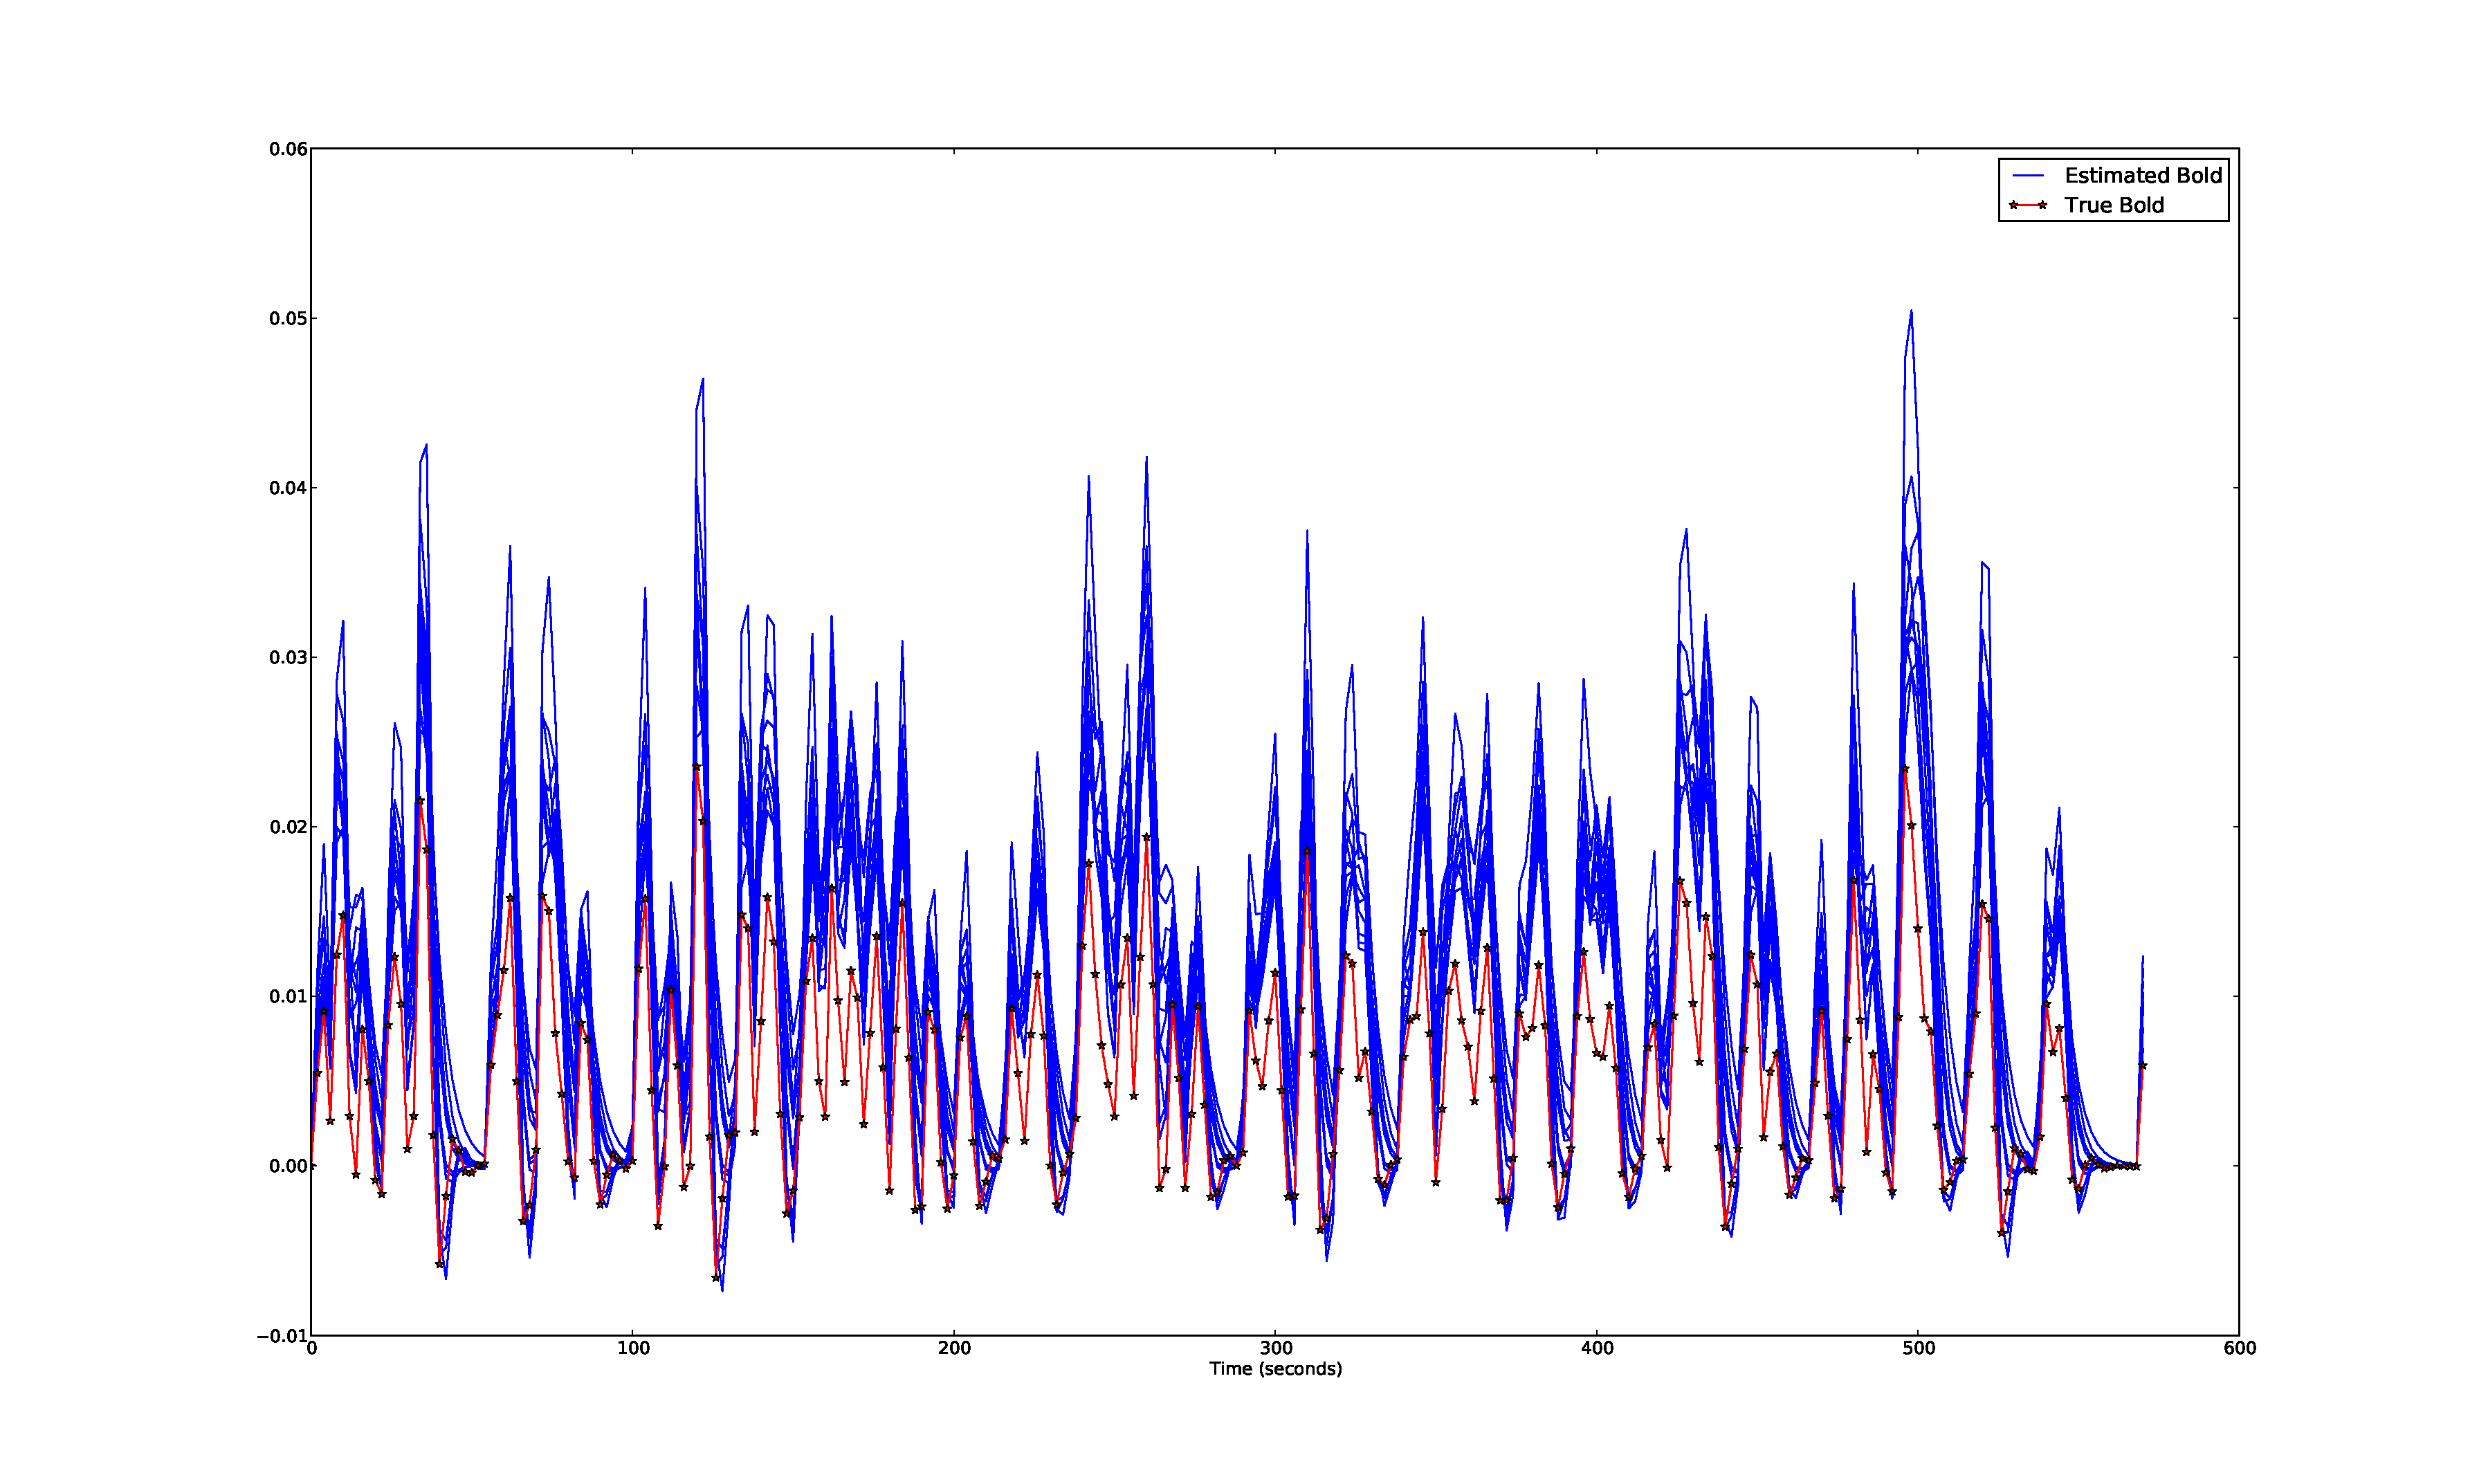
\includegraphics[clip=true,trim=6cm 2cm 5cm 3.5cm,width=15cm]{images/comparison_highnoise}
\caption{A comparison of the fitted signals for the high noise case.}
\label{fig:FitComparisonHighNoise}
\end{figure}

\begin{figure}
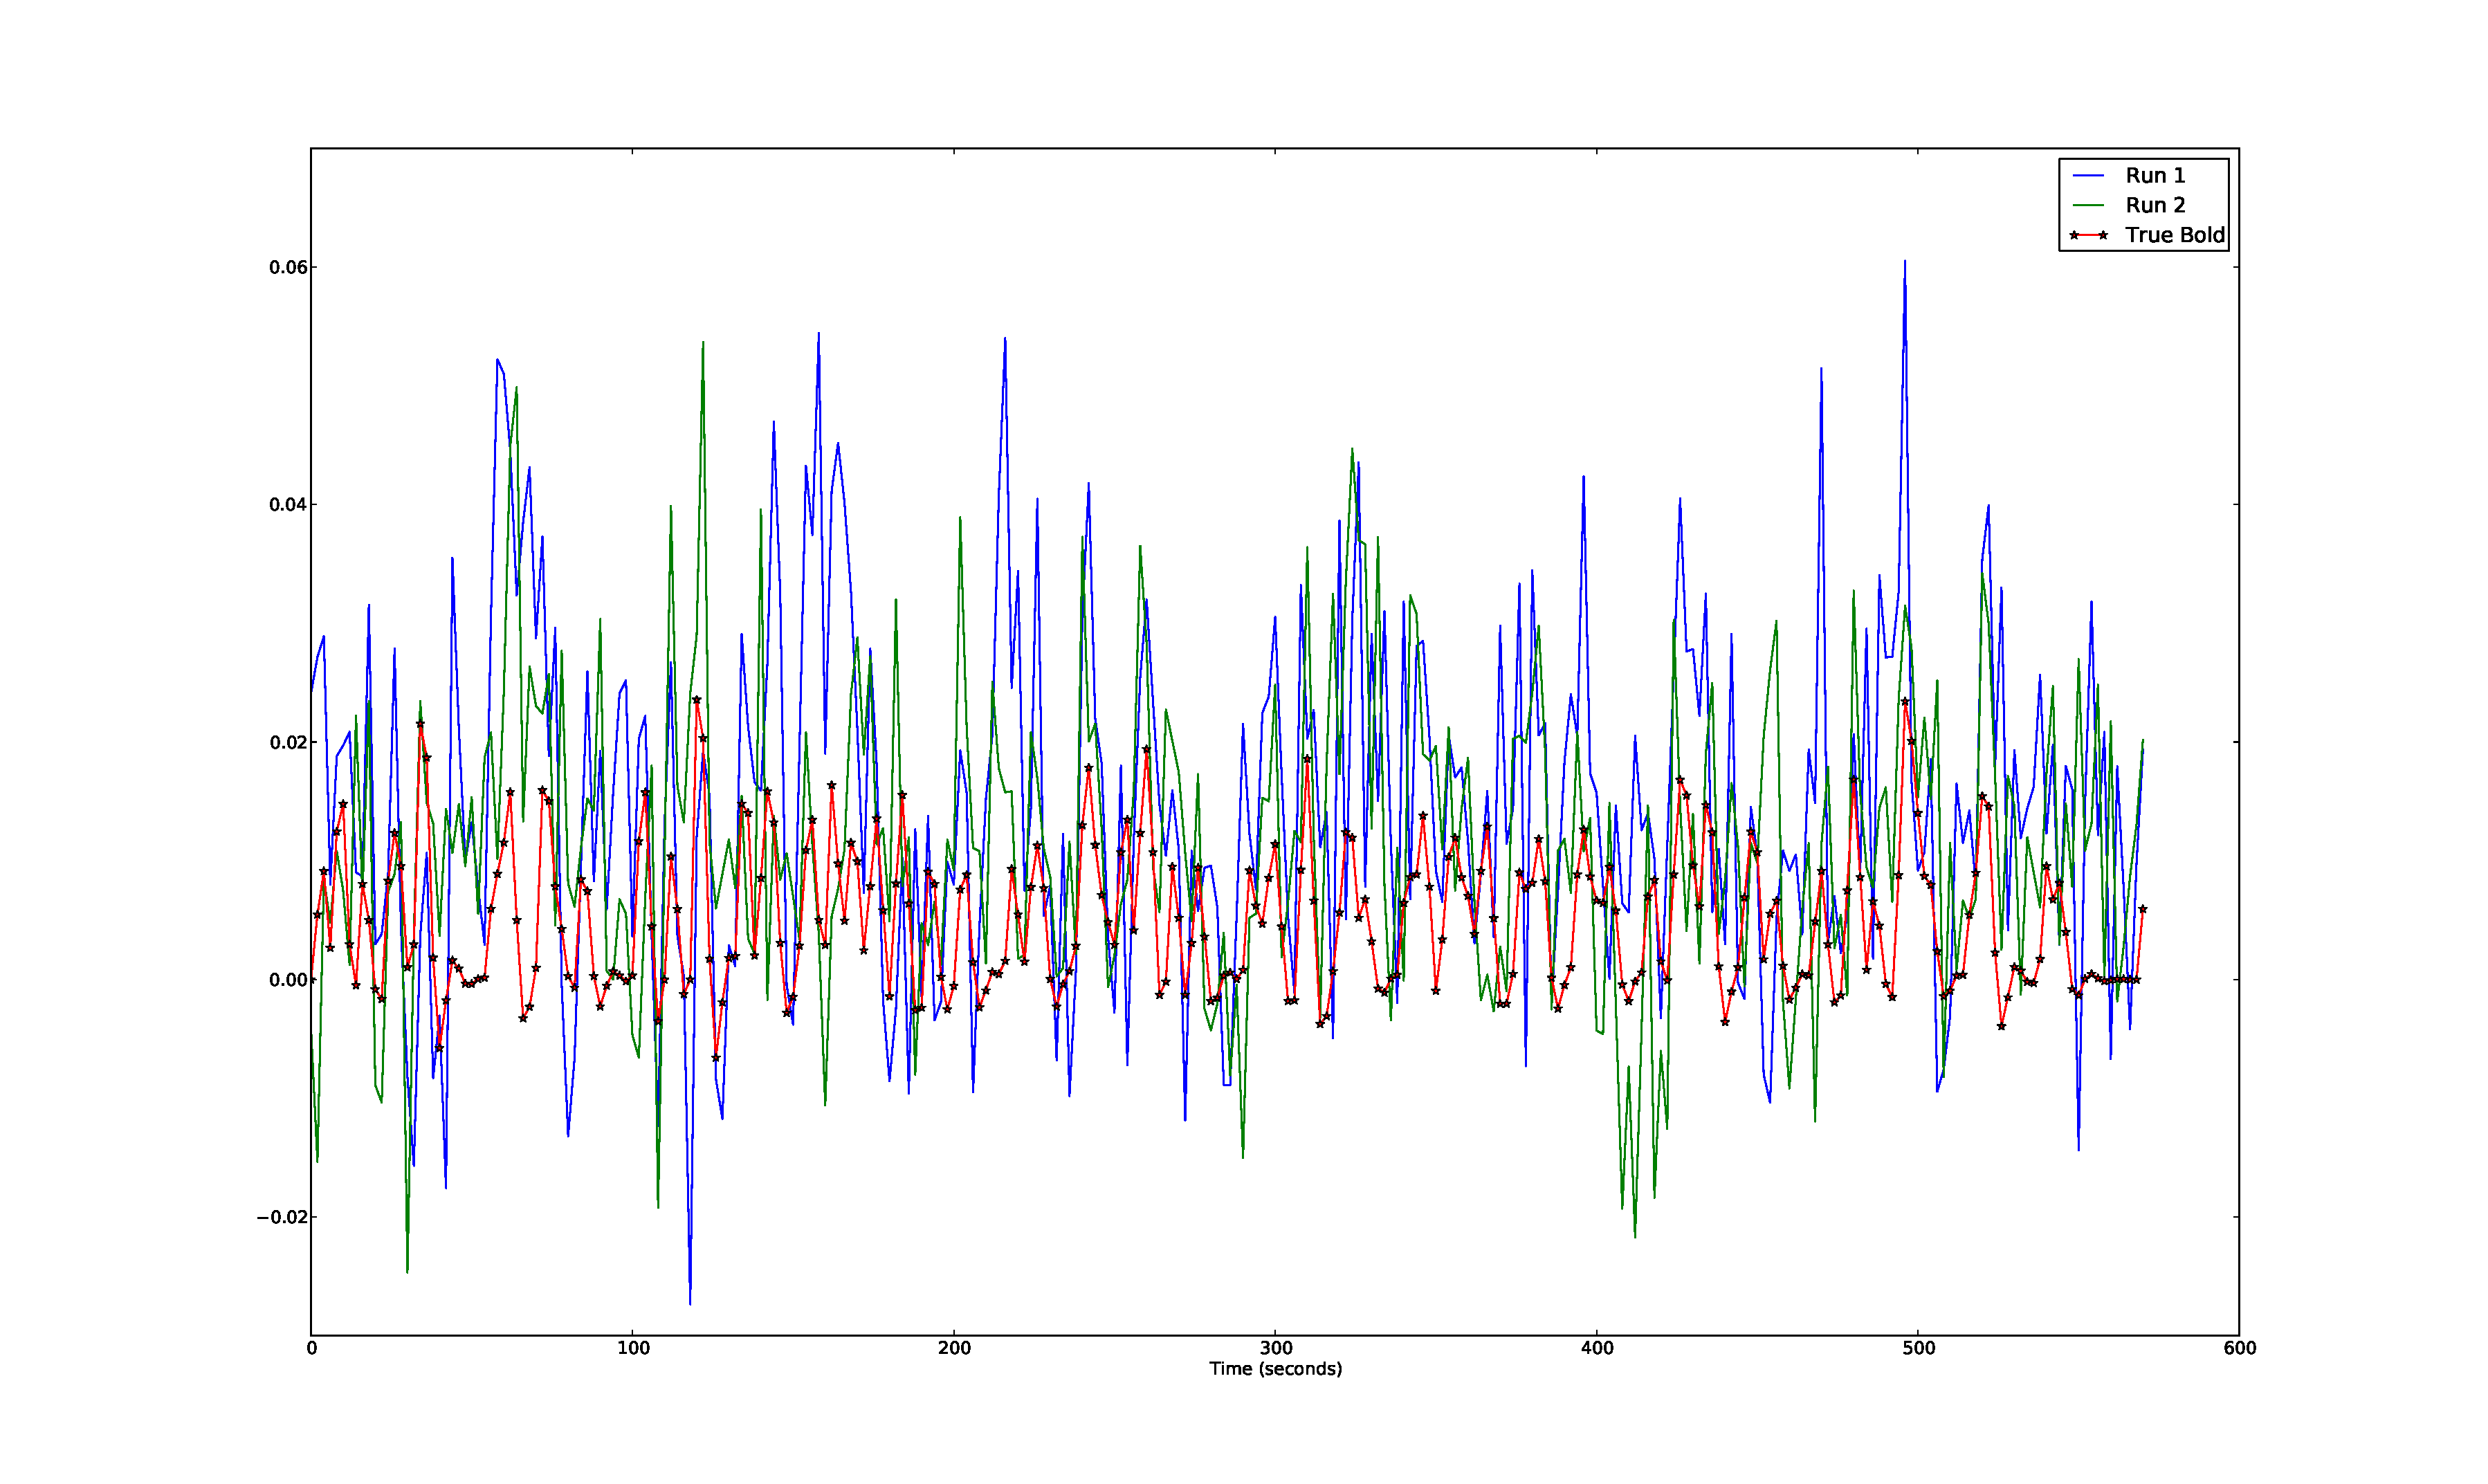
\includegraphics[clip=true,trim=6cm 2cm 5cm 3.5cm,width=15cm]{images/highnoise_56_noise}
\caption{Two particular preprocessed noise realizations for the high noise case.}
\label{fig:NoiseComparisonJustTwo}
\end{figure}

\begin{figure}
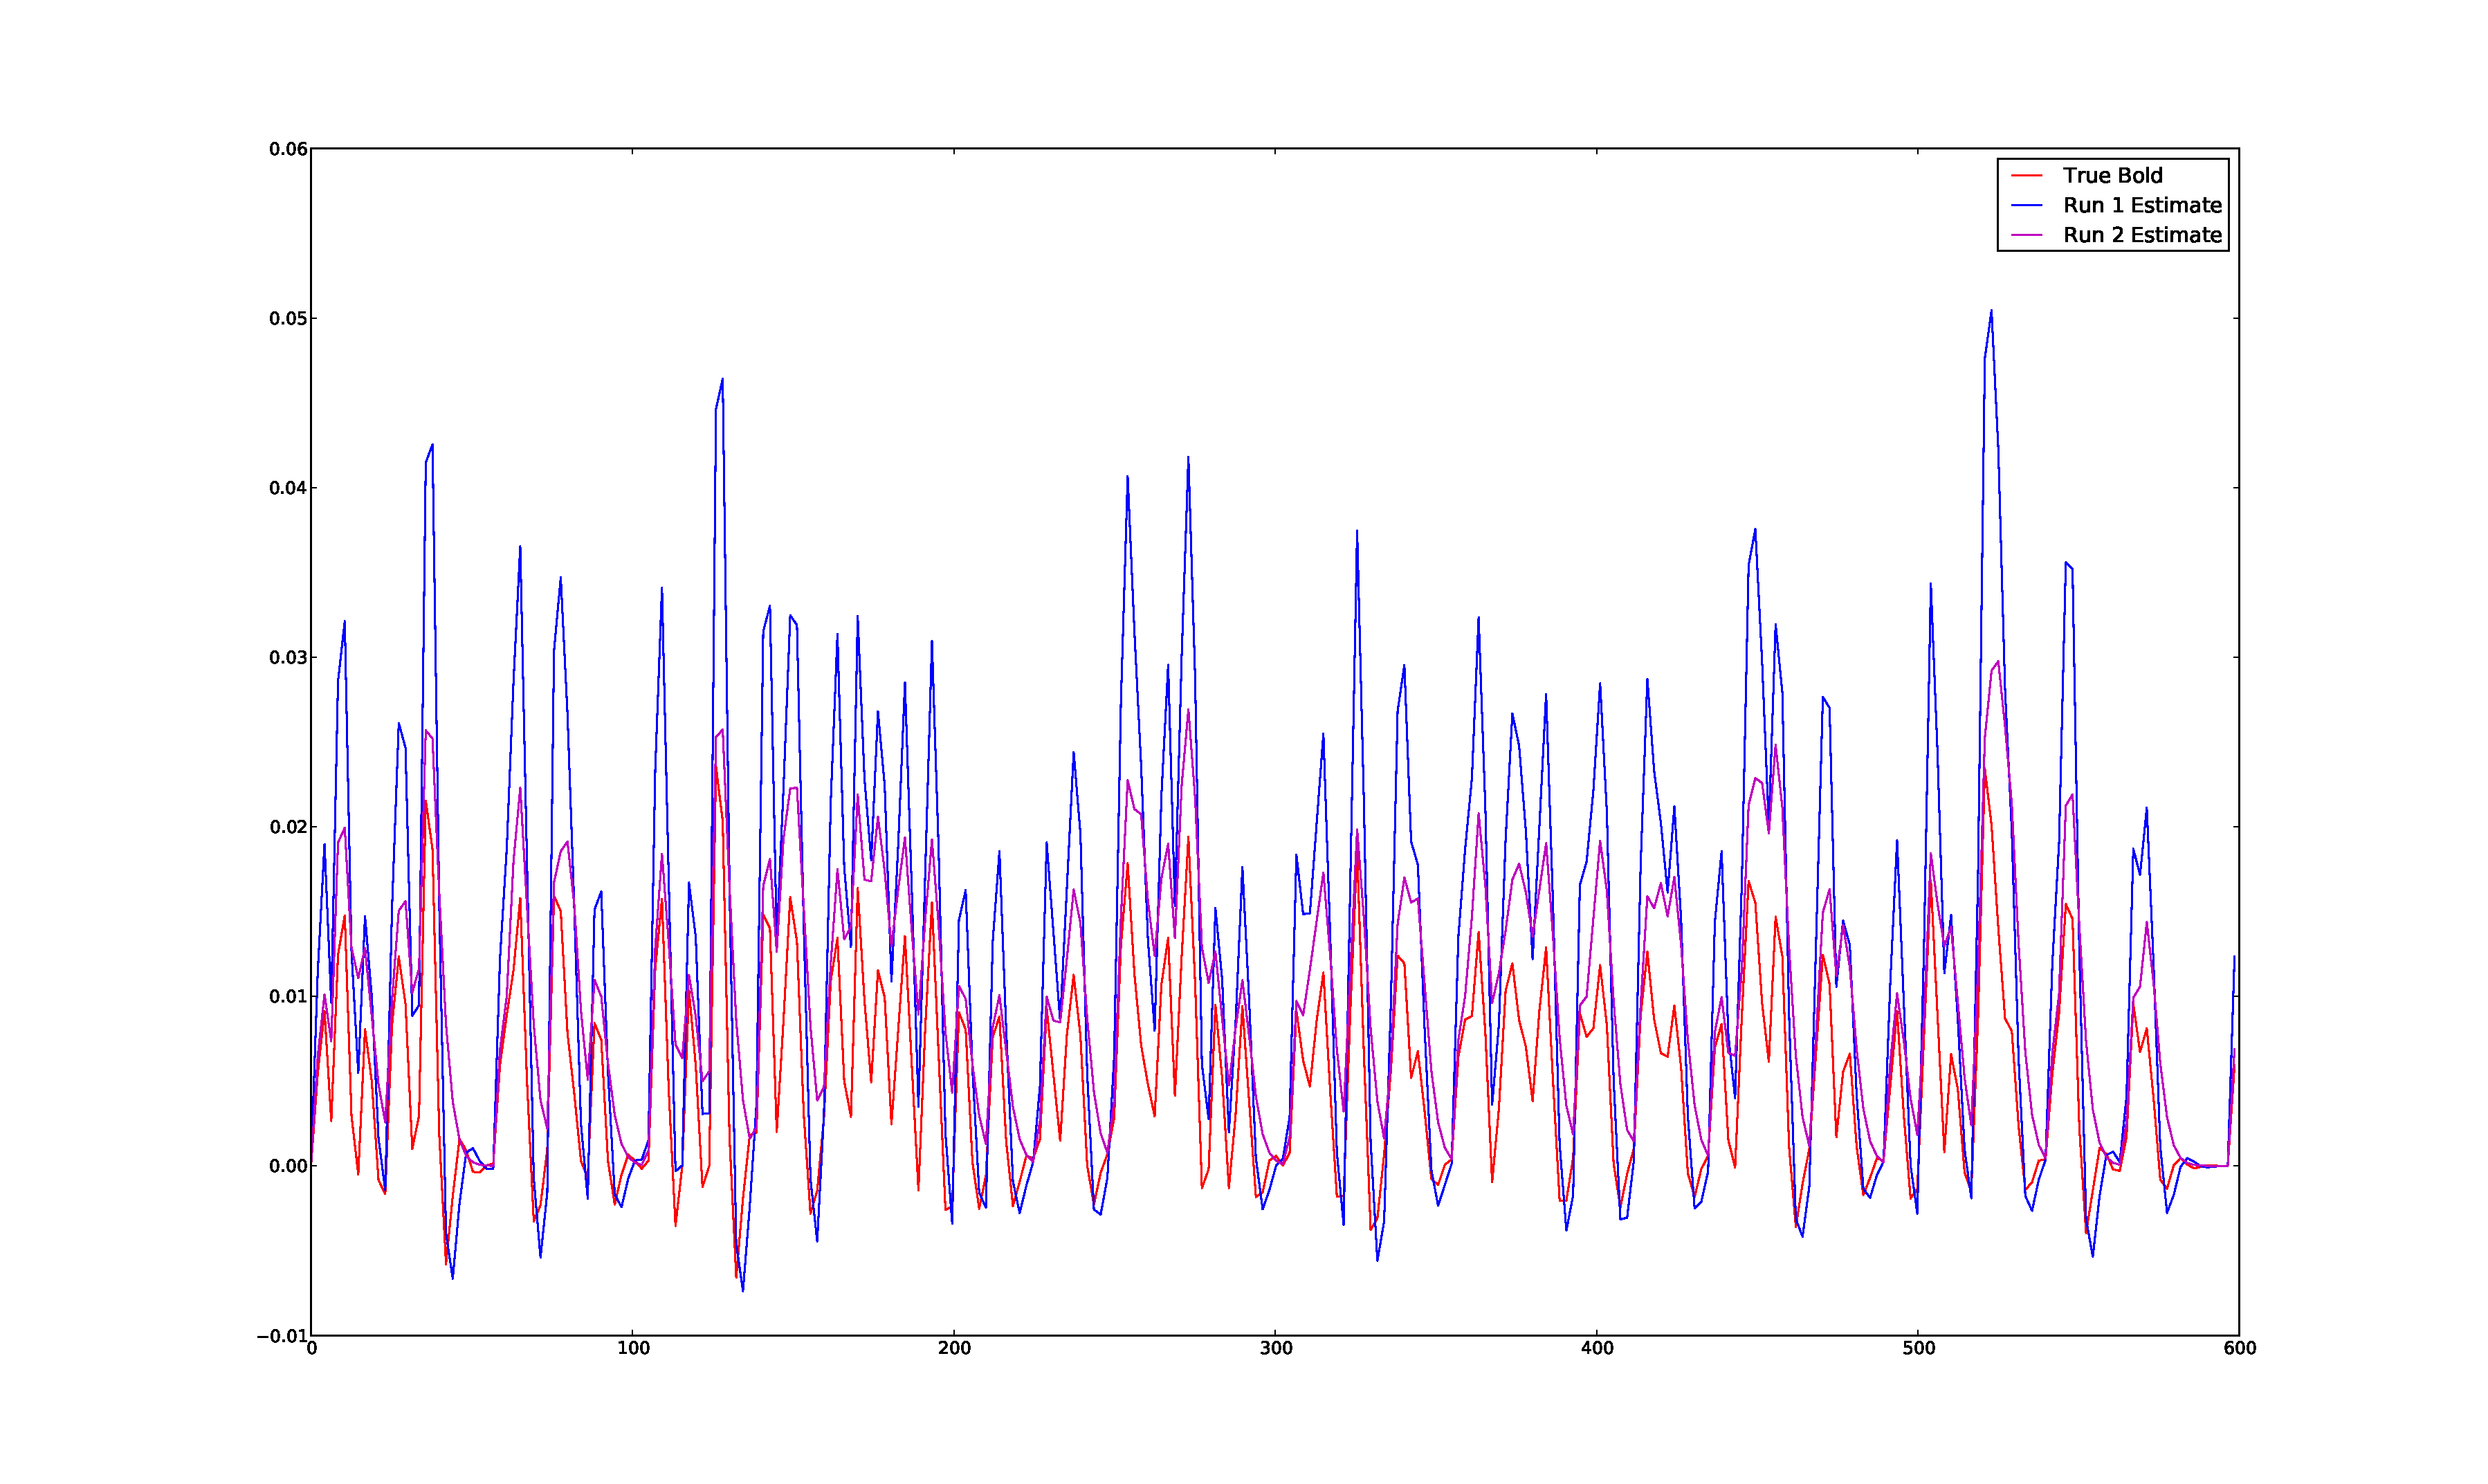
\includegraphics[clip=true,trim=6cm 2cm 5cm 3.5cm,width=15cm]{images/comparison_highnoise_just2}
\caption{The results for the noise realizations shown in \autoref{fig:NoiseComparisonJustTwo}.}
\label{fig:FitComparisonHighNoiseJust2}
\end{figure}

For the high noise simulation, the exact same procedure was followed as in \autoref{sec:SimLowNoise}
except that $\sigma_y$ and $\sigma_x$ were set to $0.01$ and $0.005$,
respectively. This is an order of magnitude higher than the previous tests, and indeed the
noise appears to dominate the output, as \autoref{fig:PreprocessedHighNoise} shows. 
The results of the particle filter
for each of the eleven runs are shown in \autoref{fig:FitComparisonHighNoise}. 
The noise and preprocessing again led the estimates
to higher peak activation levels, and the subtleties of different time constants 
are being lost in the noise. 

\begin{table}[t]
\centering
\begin{tabular}{|c | c | c | c | c | c | c | c | c | c |}
\hline 
$\tau_0$ & $\alpha$ & $E_0$    & $V_0$    & $\tau_s$ & $\tau_f$ & $\epsilon$  & $ \sum \tau $ & Residual  & Error\\
\hline 
\rowcolor[gray]{.8}
1.45 & 0.3 & 0.47 & 0.044 & 1.94 & 1.99 & 1.8  & 5.38 &  & \\
\hline 
\hline 
1.1900 & 0.2349 & 0.4223 & 0.128  & 1.0147 & 2.4779 & 1.1168 & 4.6826 &0.01406 &0.01573   \\
0.9721 & 0.2190 & 0.3051 & 0.061  & 0.5780 & 1.9960 & 3.4613 & 3.5461 &0.01373 &0.01378   \\
1.5795 & 0.1415 & 0.3380 & 0.1089 & 0.5843 & 2.1247 & 1.7834 & 4.2885 &0.01275 &0.01577   \\
1.1094 & 0.2374 & 0.5349 & 0.0351 & 1.2186 & 3.0736 & 2.3504 & 5.4016 &0.01673 &0.01154    \\
1.1071 & 0.2753 & 0.3365 & 0.0316 & 1.5057 & 2.6518 & 4.1910 & 5.2646 &0.01370 &0.01222   \\
0.5803 & 0.4793 & 0.4135 & 0.1189 & 0.9756 & 3.6902 & 1.0008 & 5.2461 &0.01150 &0.01316   \\
\rowcolor[rgb]{.9,.5,.5}
1.2952 & 0.2596 & 0.2756 & 0.2595 & 1.7026 & 2.8458 & 0.6617 & 5.8436 &0.01555 &0.01790   \\
\rowcolor[rgb]{.5,.5,.9}
1.5185 & 0.2199 & 0.2835 & 0.0742 & 0.8882 & 3.0771 & 1.7393 & 5.4838 &0.01205 &0.01246   \\
0.6874 & 0.3283 & 0.3979 & 0.1561 & 1.0778 & 3.1158 & 0.6643 & 4.8810 &0.01510 &0.01258   \\
1.0170 & 0.285  & 0.3474 & 0.0567 & 1.5877 & 2.6516 & 2.2852 & 5.2563 &0.01249 &0.01343   \\
0.9925 & 0.298  & 0.3221 & 0.2094 & 0.4276 & 2.2108 & 1.0167 & 3.6308 &0.01217 &0.01506   \\
\hline                                                                          
1.0954 & 0.2708 & 0.3615 & 0.1126 & 1.0510 & 2.7196 & 1.8428 & 4.8659 &0.01362 &0.01397\\
\hline 
\end{tabular}
\caption{Estimated Parameters on 11 different runs with high noise. First row contains the true parameters,
last row contains the mean.
The red row is Run 1 and the blue row is Run 2 from  \autoref{fig:NoiseComparisonJustTwo}
and \autoref{fig:FitComparisonHighNoiseJust2}, respectively.}
\label{tab:HighNoiseResults} 
\end{table}

\autoref{fig:NoiseComparisonJustTwo} shows two of the runs in more detail.
There appears
to be more drift than the 20 measurements per knot could fit, which explains 
the prolonged increase at 170 seconds in Run 1; although such areas
permeate the preprocessed signals.
Interestingly, Run 1 and Run 2 emphasize
different aspects of the signal. Run 2 had a much better match to the 
peaks, when compared to the true signal, yet Run 1 matched the post-stimulus
undershoot better.  \autoref{tab:HighNoiseResults} shows
the error  for all eleven runs, and highlights the two runs analyzed 
in \autoref{fig:ConvergenceRuns1} and \autoref{fig:ConvergenceRuns2}.

\begin{figure}[H]
\subfigure[$\tau_0$, $\alpha$, $E_0$, $V_0$, Run 1]
{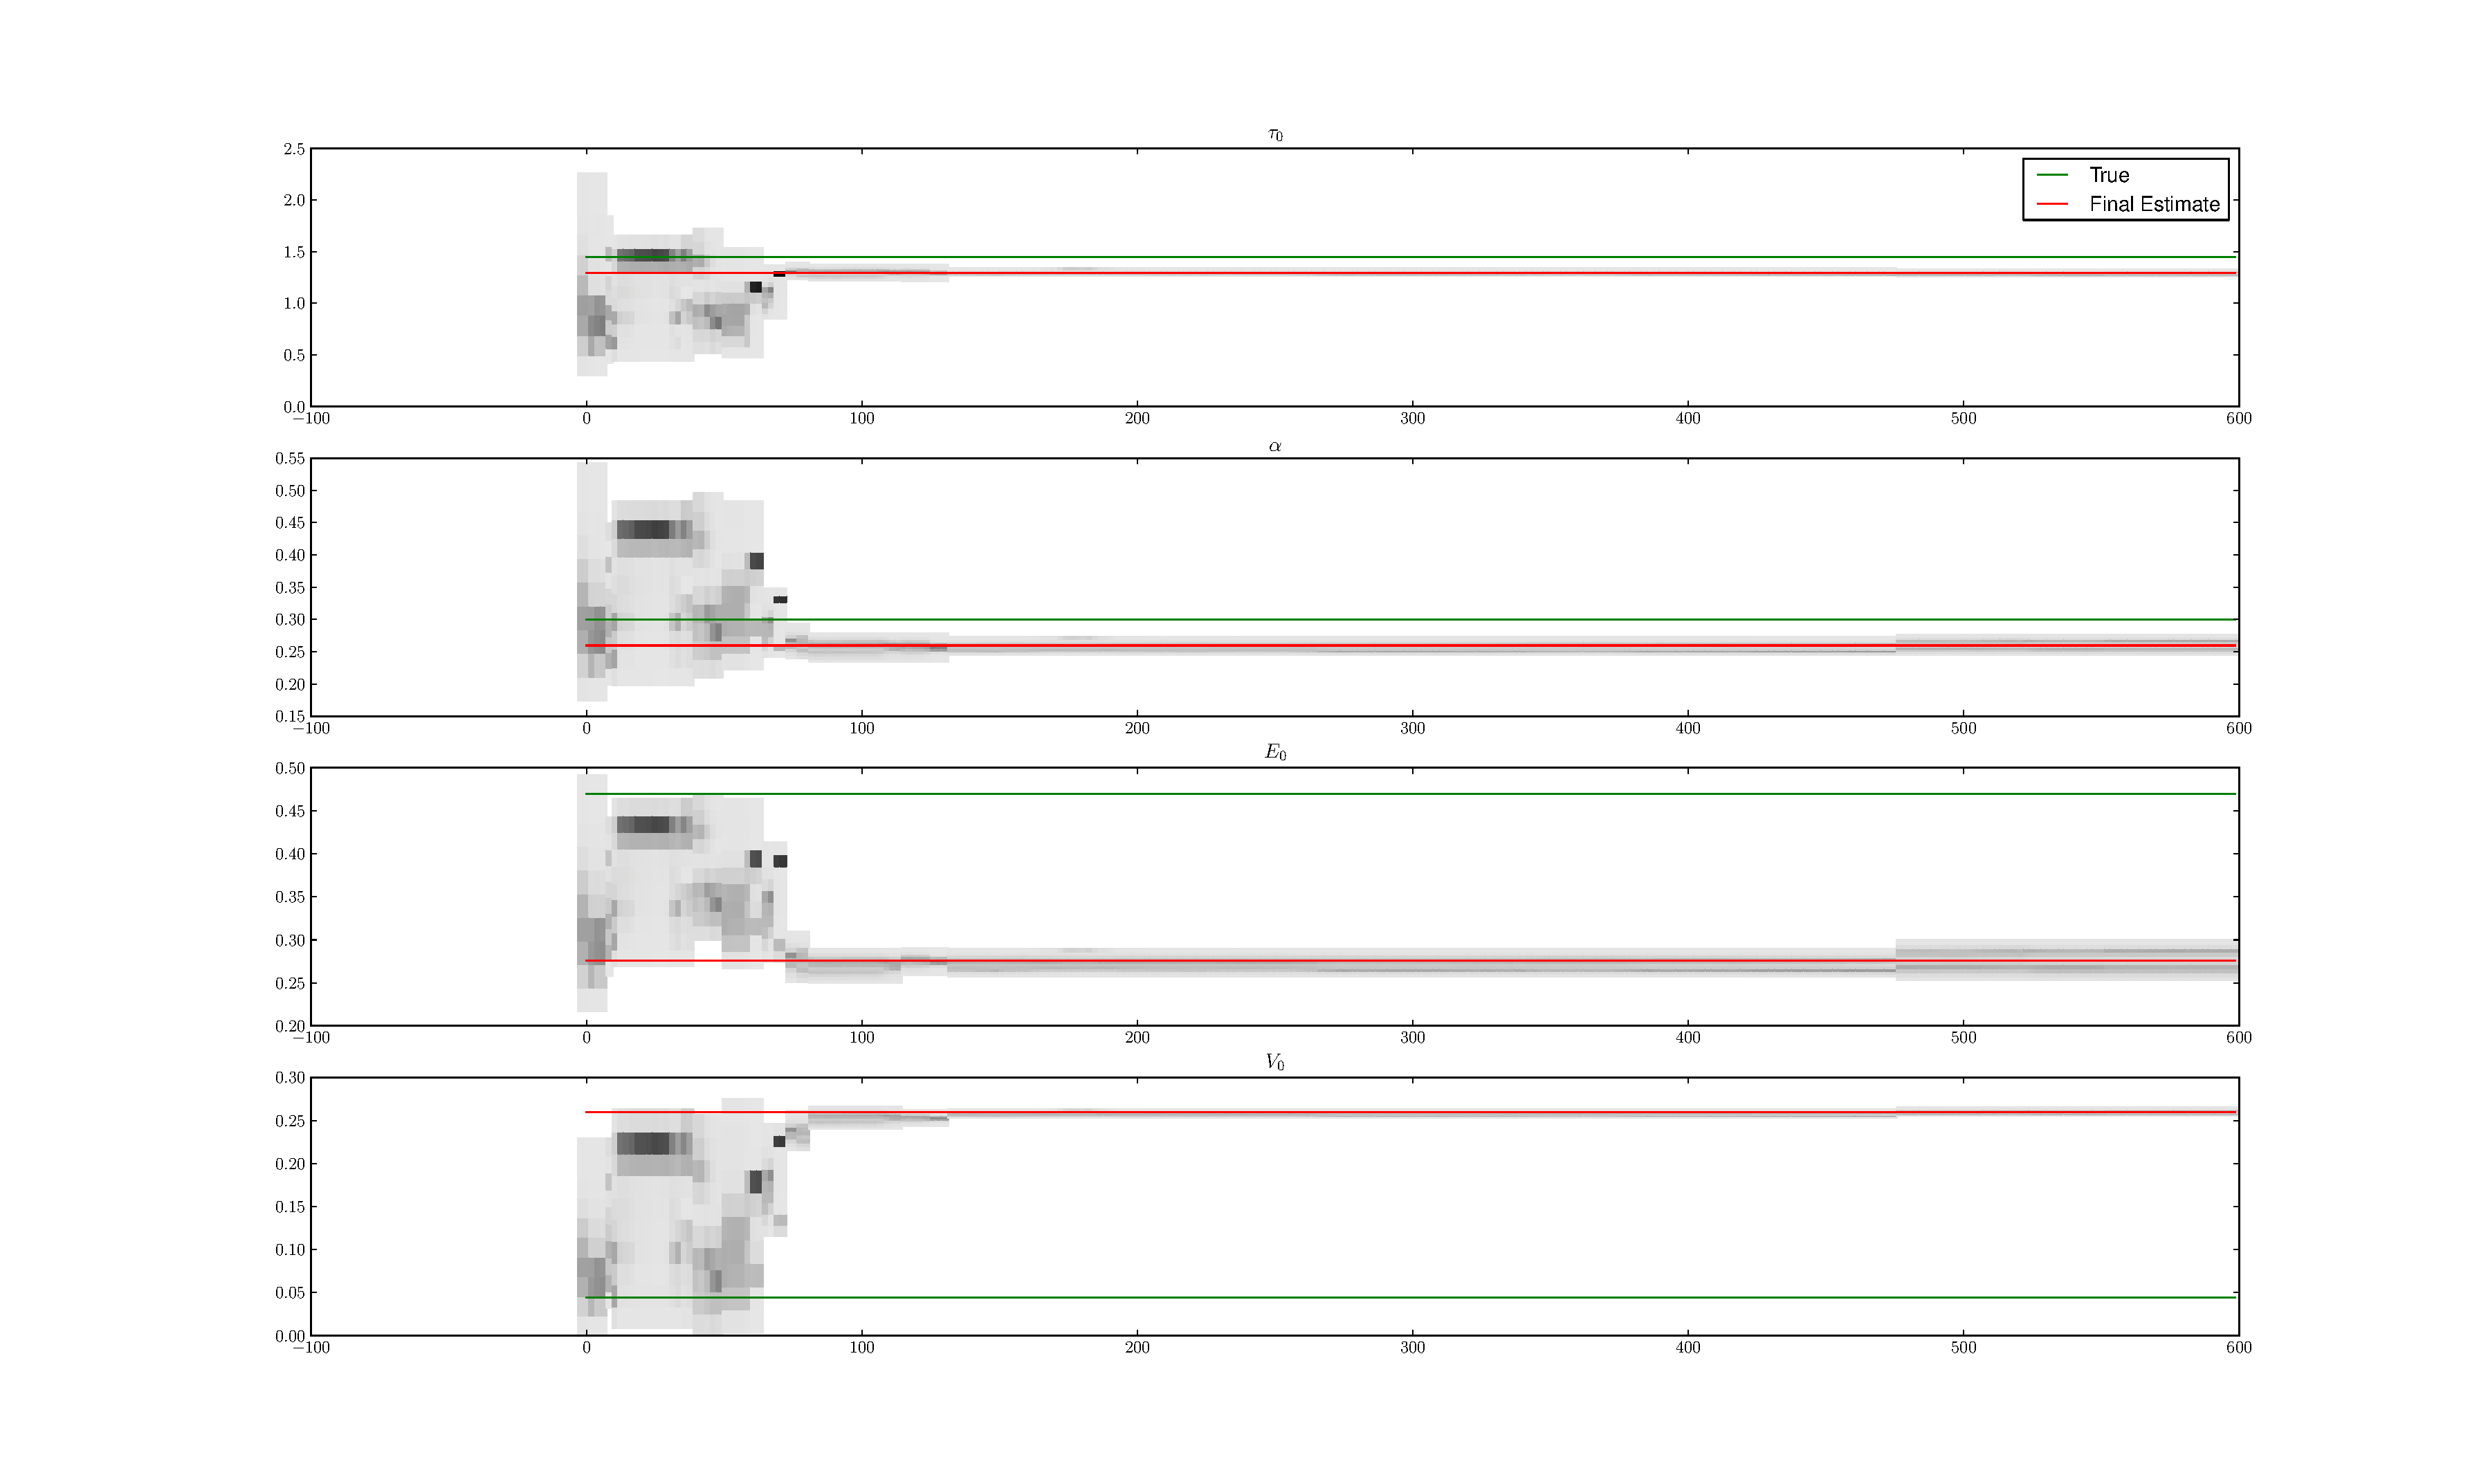
\includegraphics[clip=true,trim=6cm 2cm 6cm 3cm, width=14cm]{images/highnoise_run5_1}}\\
\end{figure}

\begin{figure}[H]
\subfigure[$\tau_s$, $\tau_f$, $\epsilon$, $v$, Run 1] 
{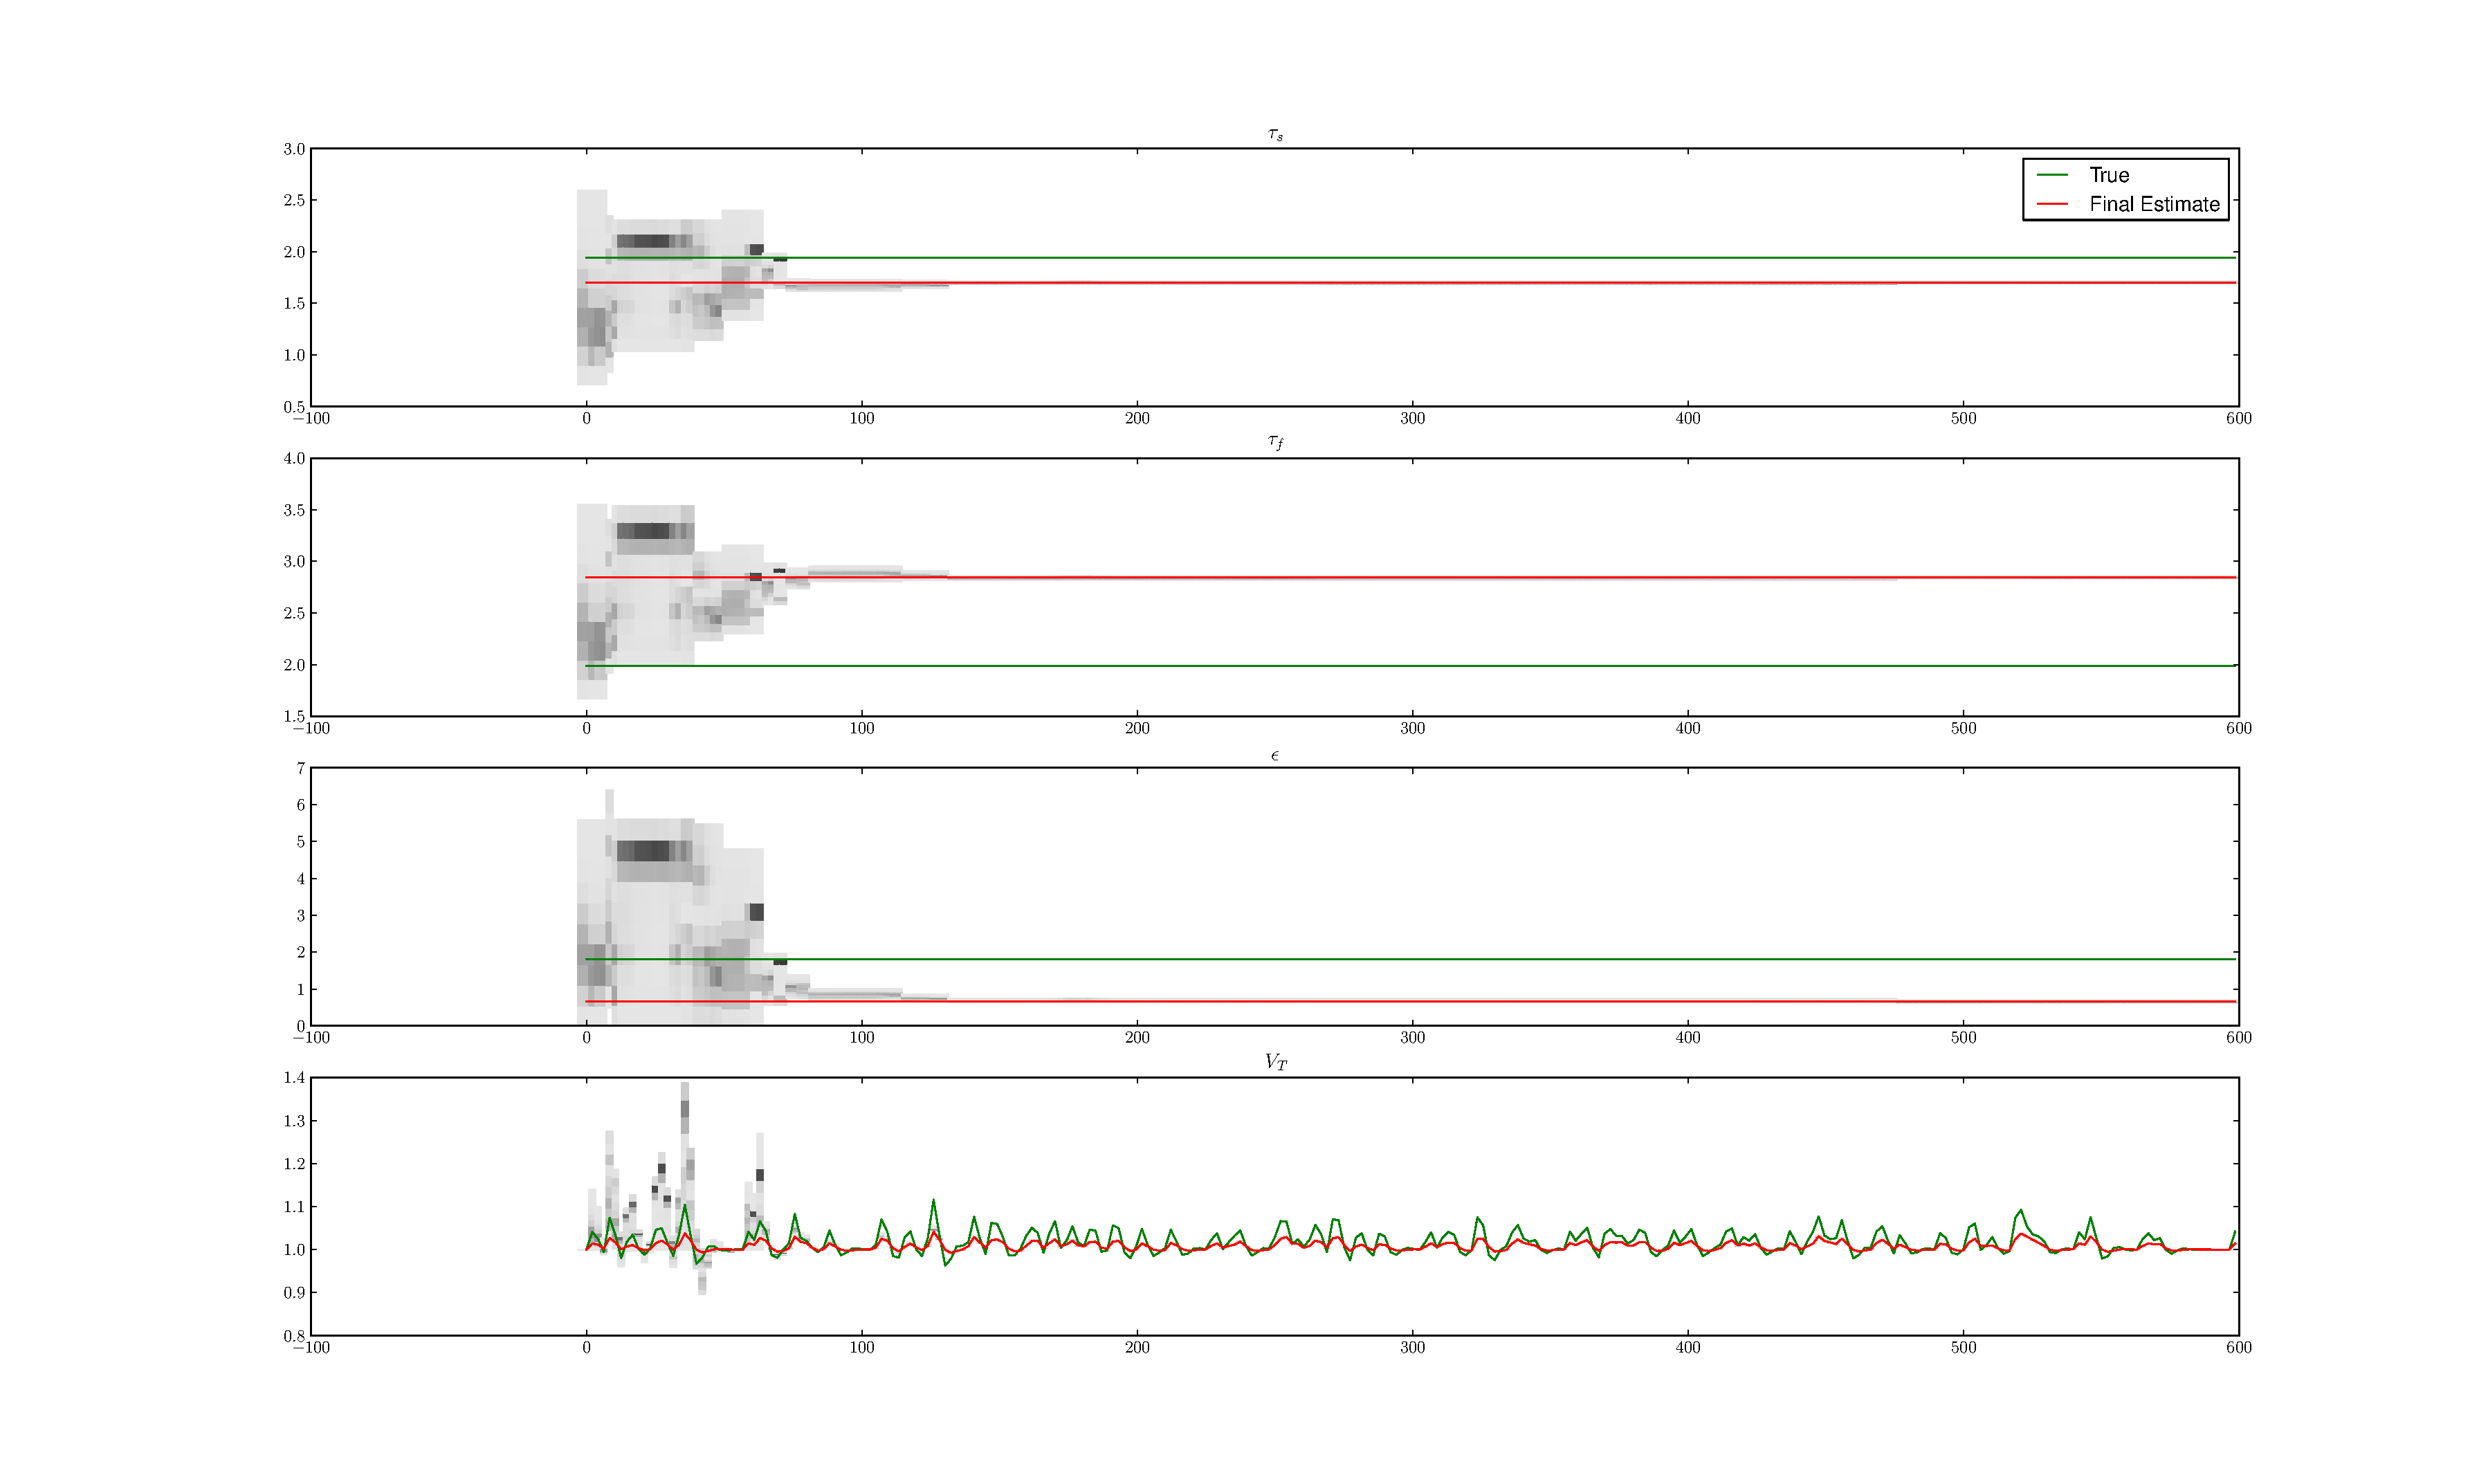
\includegraphics[clip=true,trim=6cm 2cm 6cm 3cm, width=14cm]{images/highnoise_run5_2}}\\
\end{figure}

\begin{figure}[H]
\subfigure[$q$, $s$, $f$, $BOLD$, Run 1 ]
{\label{fig:ConvergenceRuns1c} 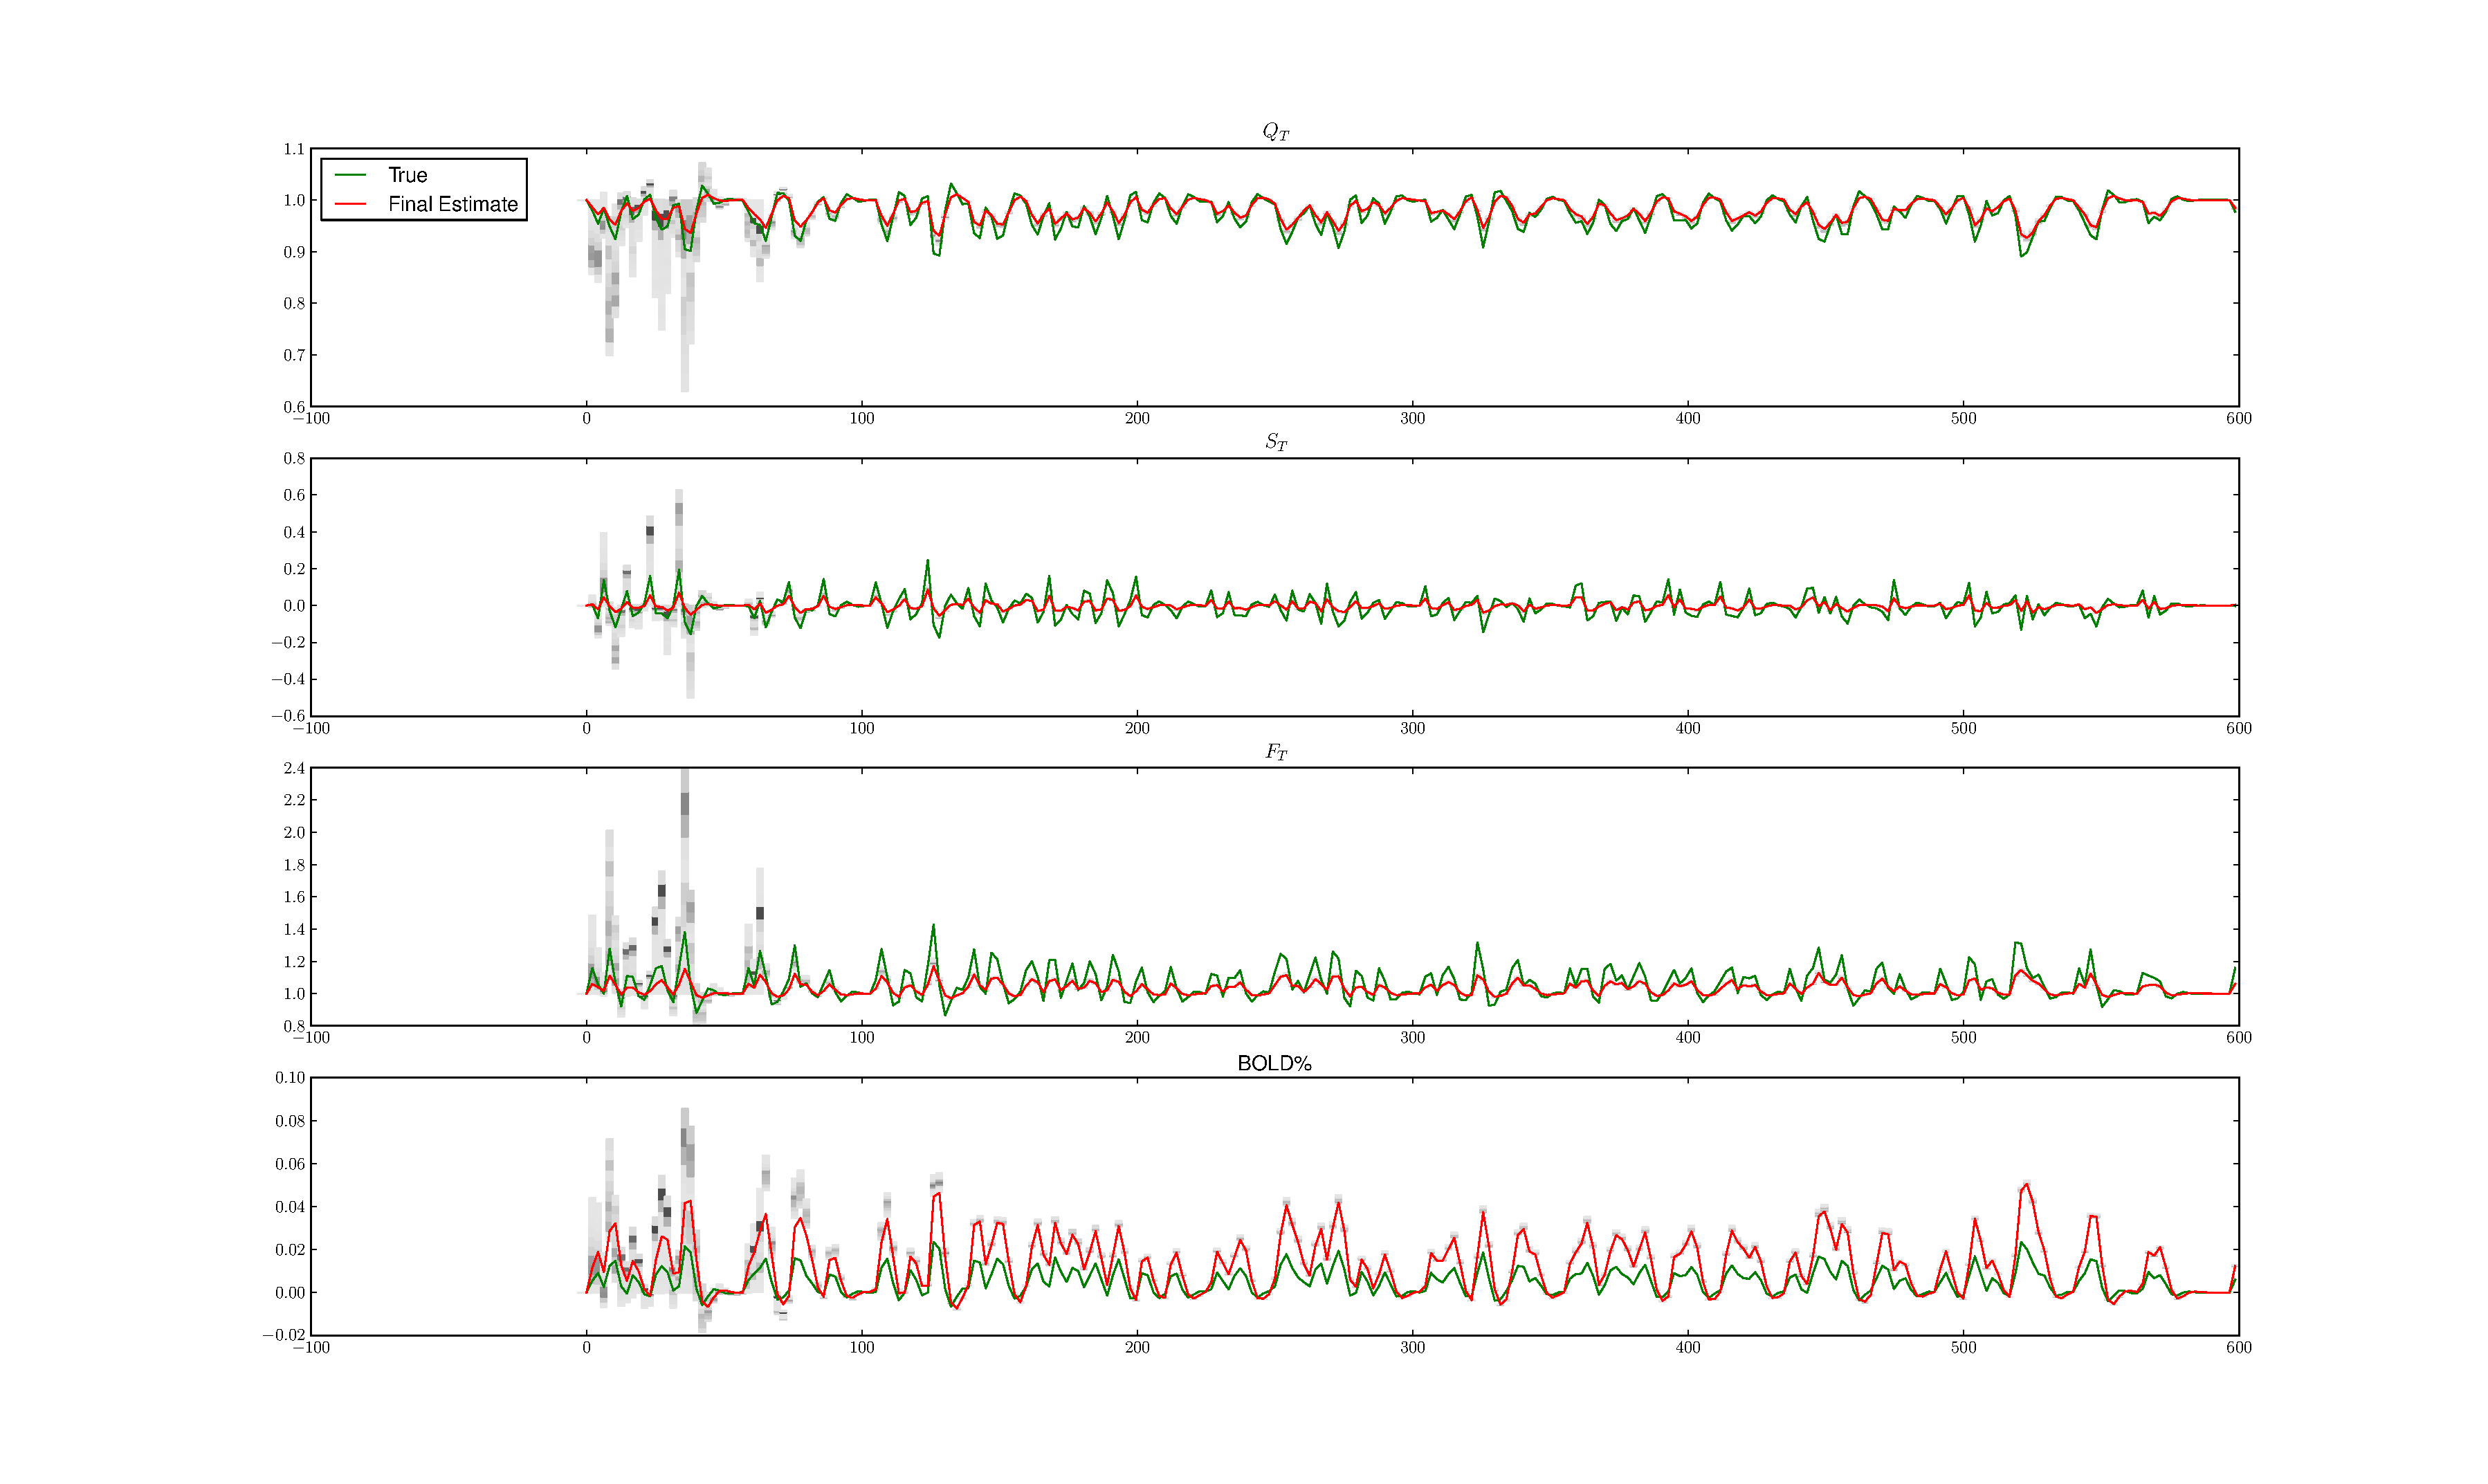
\includegraphics[clip=true,trim=6cm 2cm 6cm 3cm, width=14cm]{images/highnoise_run5_3}}
\caption{Converging histogram for parameters during run 1, as in \autoref{fig:NoiseComparisonJustTwo}.}
\label{fig:ConvergenceRuns1}
\end{figure}

\begin{figure}[H]
\subfigure[$\tau_0$, $\alpha$, $E_0$, $V_0$, Run 2]
{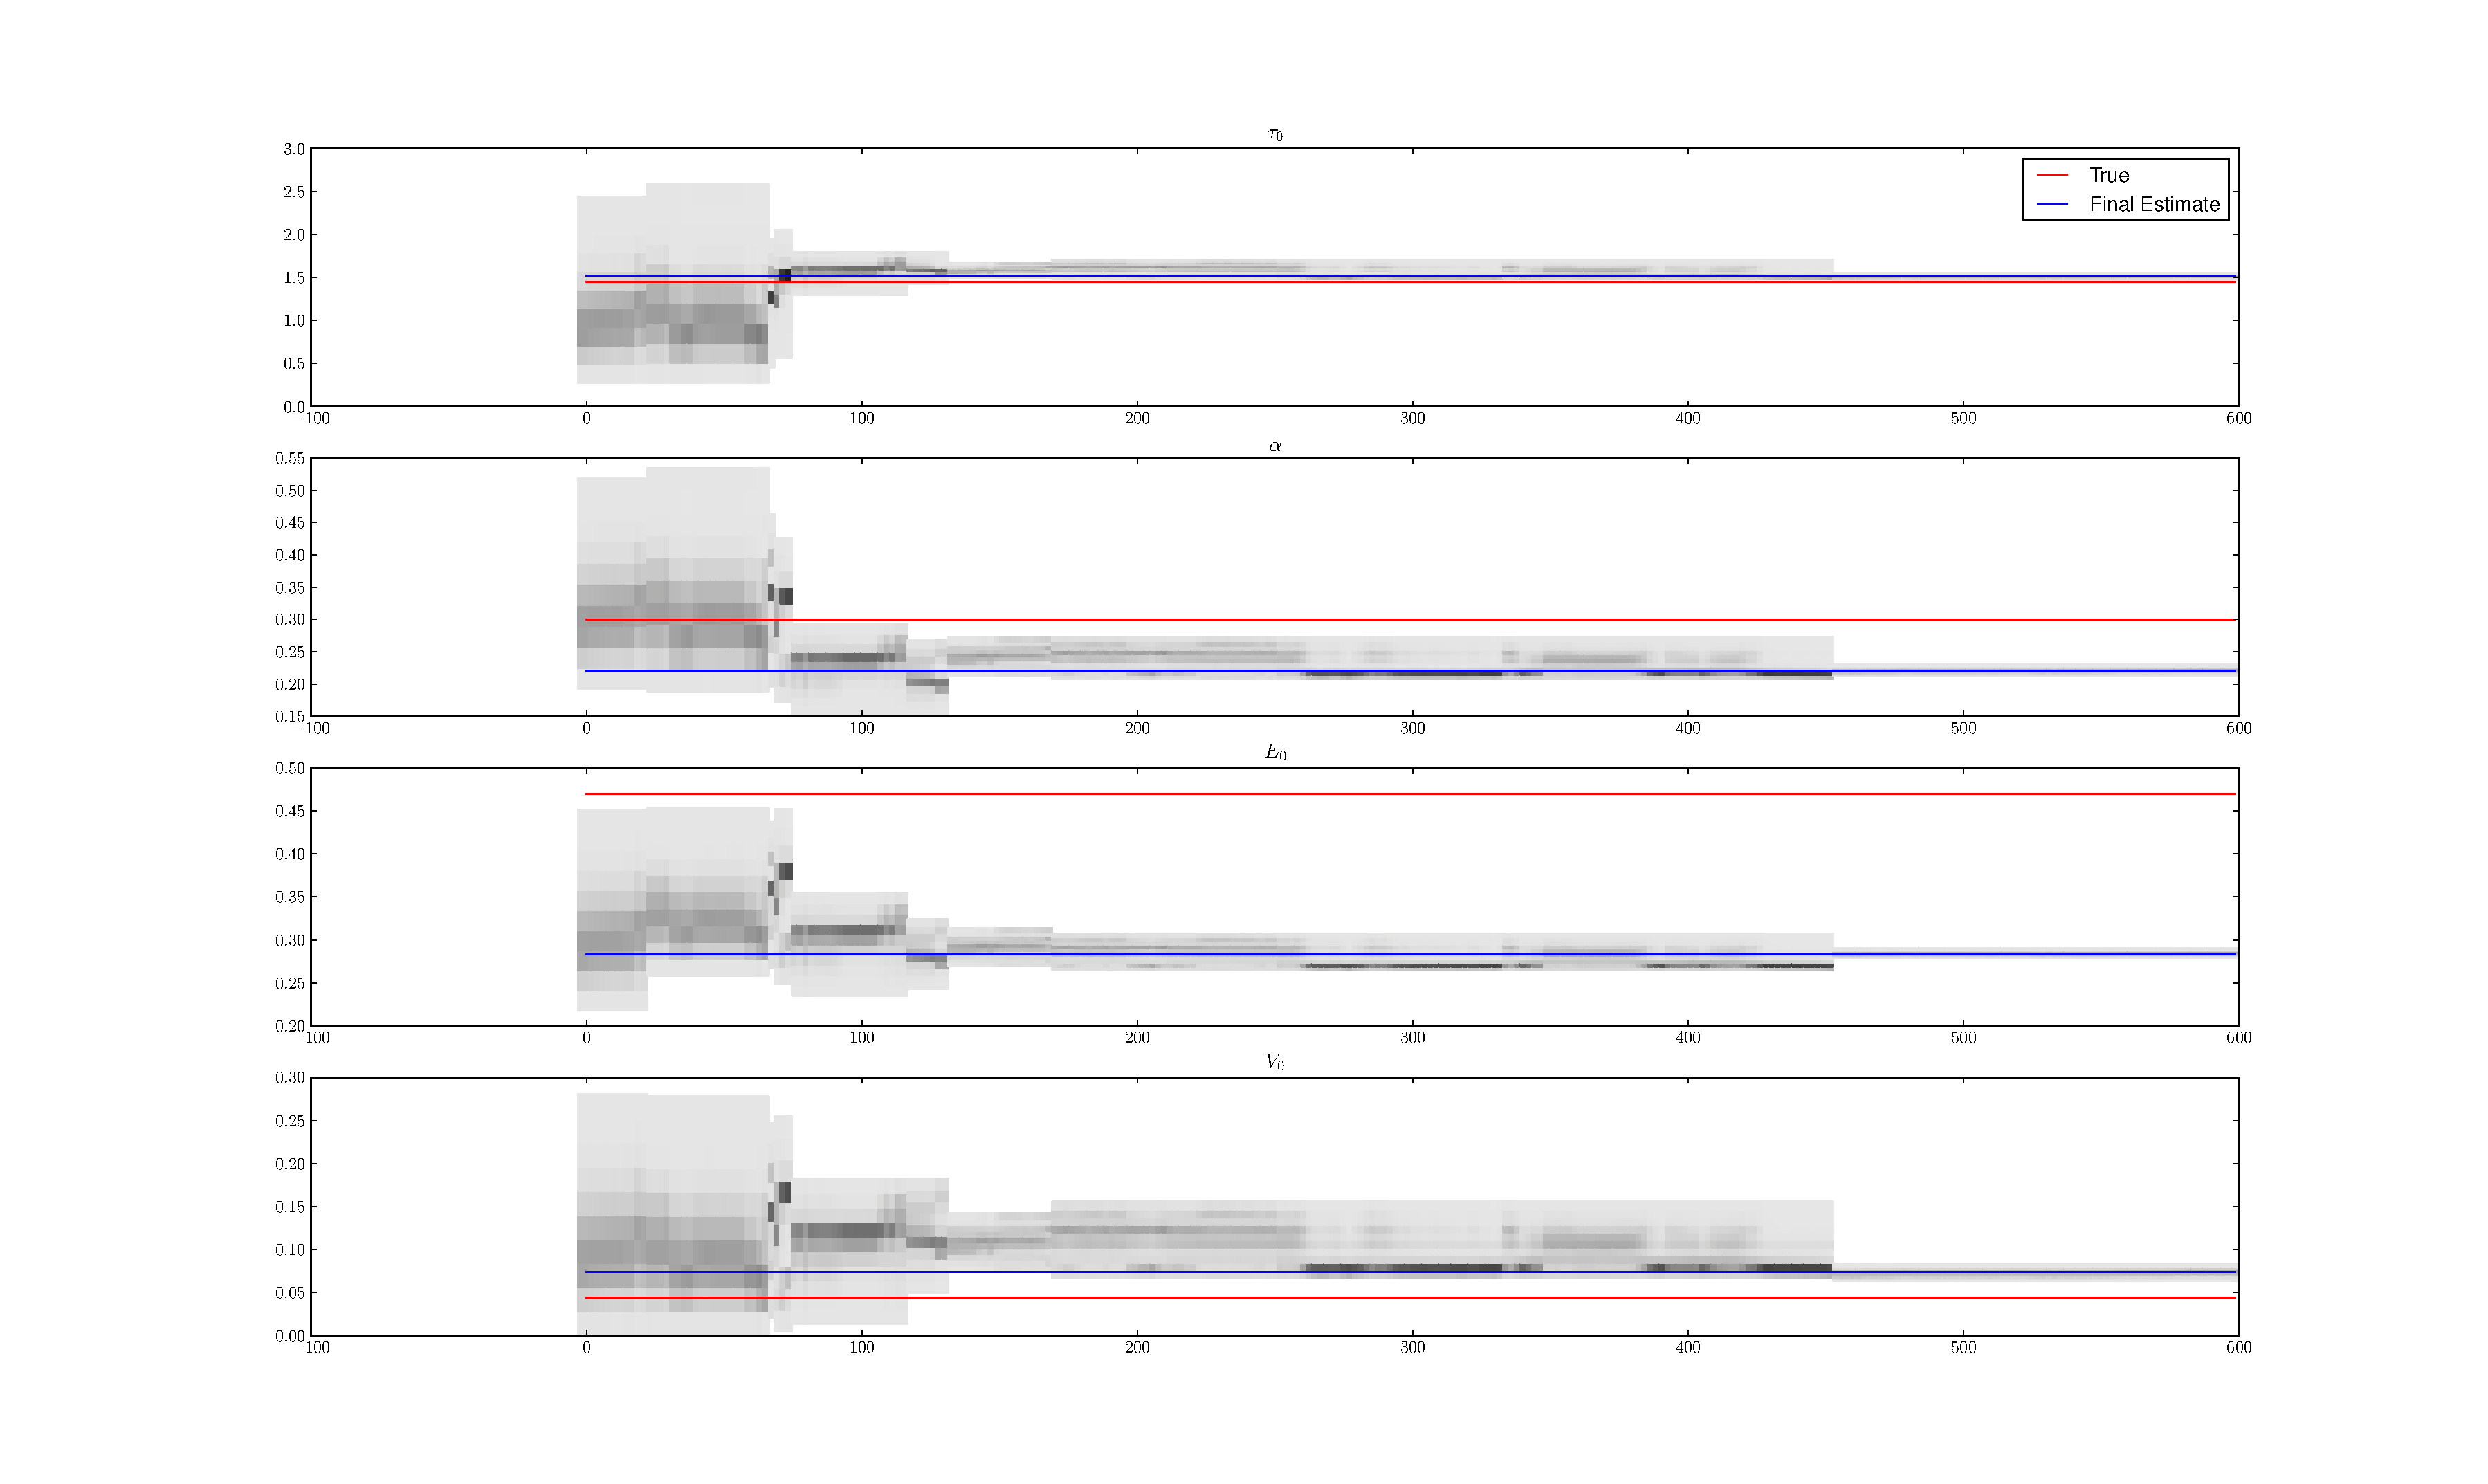
\includegraphics[clip=true,trim=6cm 2cm 6cm 3cm, width=14cm]{images/highnoise_run6_1}}\\
\end{figure}

\begin{figure}[H]
\subfigure[$\tau_s$, $\tau_f$, $\epsilon$, $v$, Run 2] 
{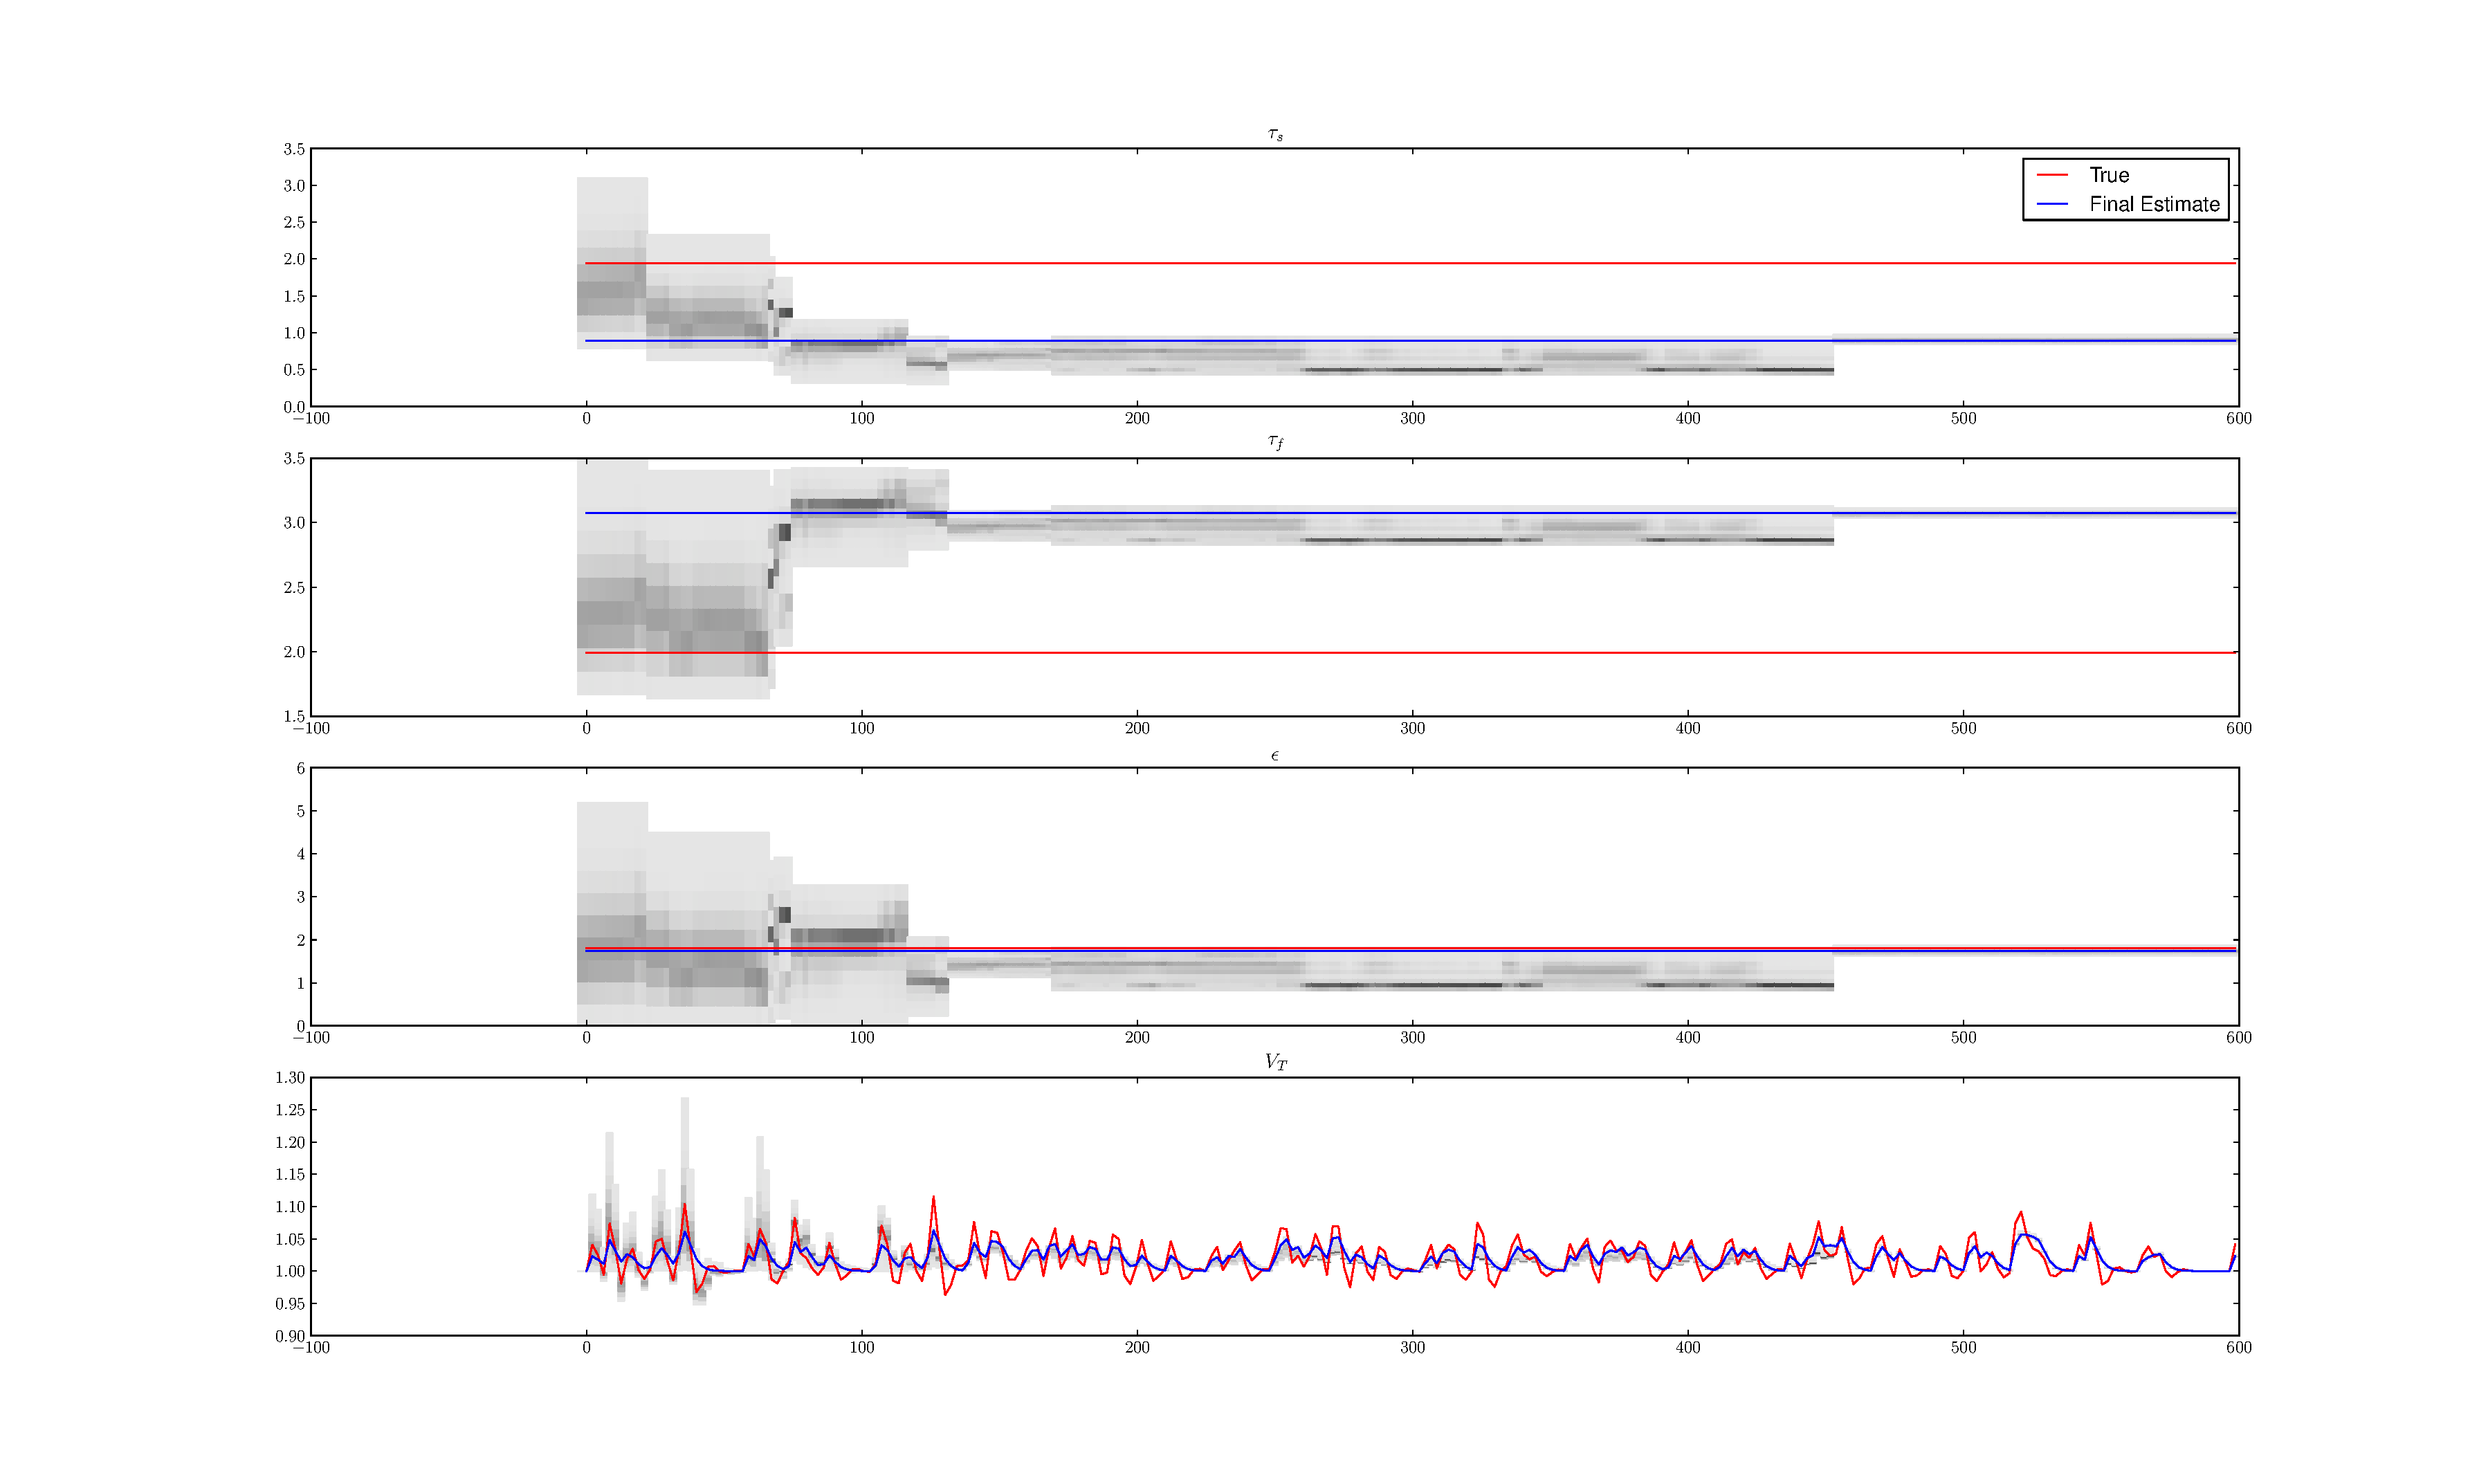
\includegraphics[clip=true,trim=6cm 2cm 6cm 3cm, width=14cm]{images/highnoise_run6_2}}\\
\end{figure}

\begin{figure}[H]
\subfigure[$q$, $s$, $f$, $BOLD$, Run 2 ]
{\label{fig:ConvergenceRuns2c} 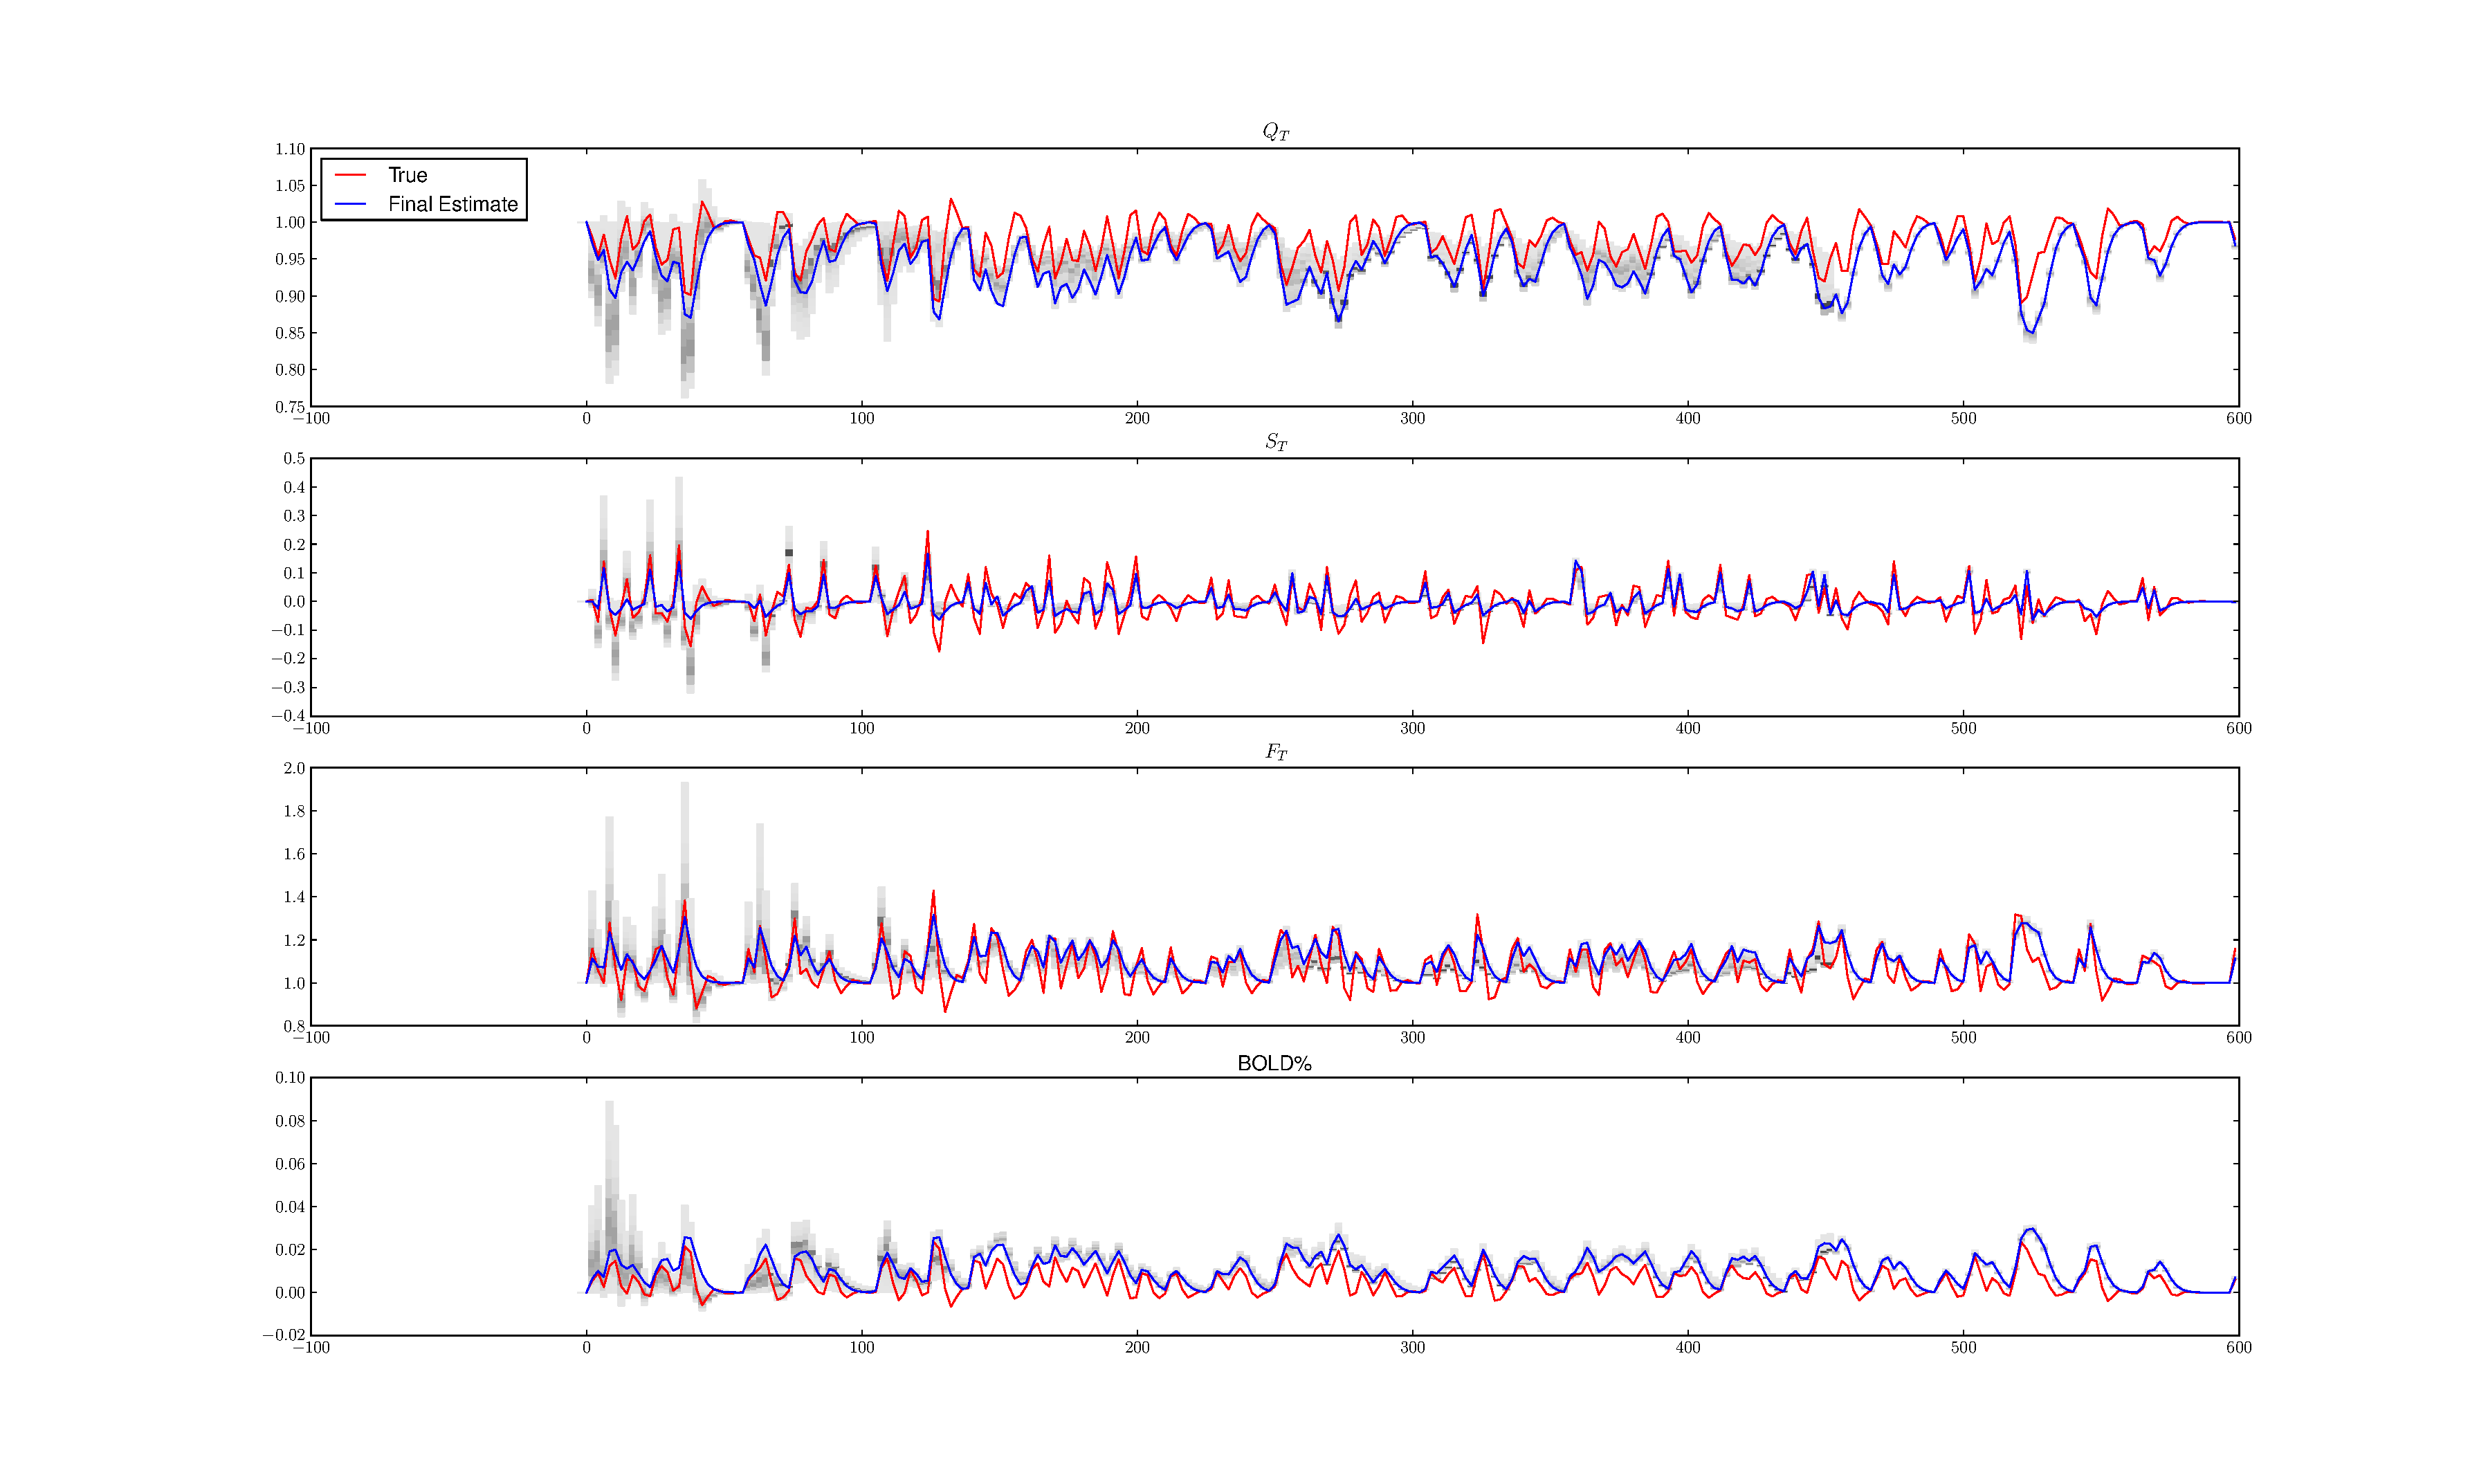
\includegraphics[clip=true,trim=6cm 2cm 6cm 3cm, width=14cm]{images/highnoise_run6_3}}
\caption{Converging histogram for parameters during run 2, as in \autoref{fig:NoiseComparisonJustTwo}.}
\label{fig:ConvergenceRuns2}
\end{figure}

The particles converged much faster when more noise was present (\autoref{fig:LowNoiseHist} vs. 
\autoref{fig:ConvergenceRuns1}, \autoref{fig:ConvergenceRuns2}). 
This also caused significantly more resampling which 
is the explanation for the perceived jumps in the histograms. 
Clearly the additional noise resulted in much more sporadic results (\autoref{tab:HighNoiseResults}). 
This is often the 
result when the particle filter converges too fast, in this case the result of the 
weighting function's variance being smaller than the measurement noise ($0.005$ vs. $0.01$). 
The error clearly suffers due to this effect (\autoref{tab:HighNoiseResults}).
Note that neither Run 1 or Run 2 estimated the underlying state well (\autoref{fig:ConvergenceRuns1c}
and \autoref{fig:ConvergenceRuns2c}), whereas
in the previous test the particle filter was extremely successful in this area (\autoref{fig:LowNoiseHistc}).

%NO SIGNAL, LOW NOISE
\subsection{Pure Noise, Low magnitude}
\label{sec:PureNoiseLowMag}
The next two single-voxel tests forced the particle filter to attempt to learn a noise-only
time series. In this test the noise was the same as that from the \autoref{sec:SimHighNoise},
$\sigma_x = 0.01, \sigma_y = 0.005$. The stimulus neuronal efficiency ($\epsilon$) was set 
to 0, in effect simulating a brain region with no response to the stimuli.
This test was used to determine how the output of a pure noise timeseries
is different from that of a simple noisy signal (as in the previous two sections). 
The preprocessed signals are shown in \autoref{fig:PreprocessedNoiseOnly}
and line fit for each run is shown in \autoref{fig:fits_noiseonly}. 

%\begin{figure}[H]
%\centering
%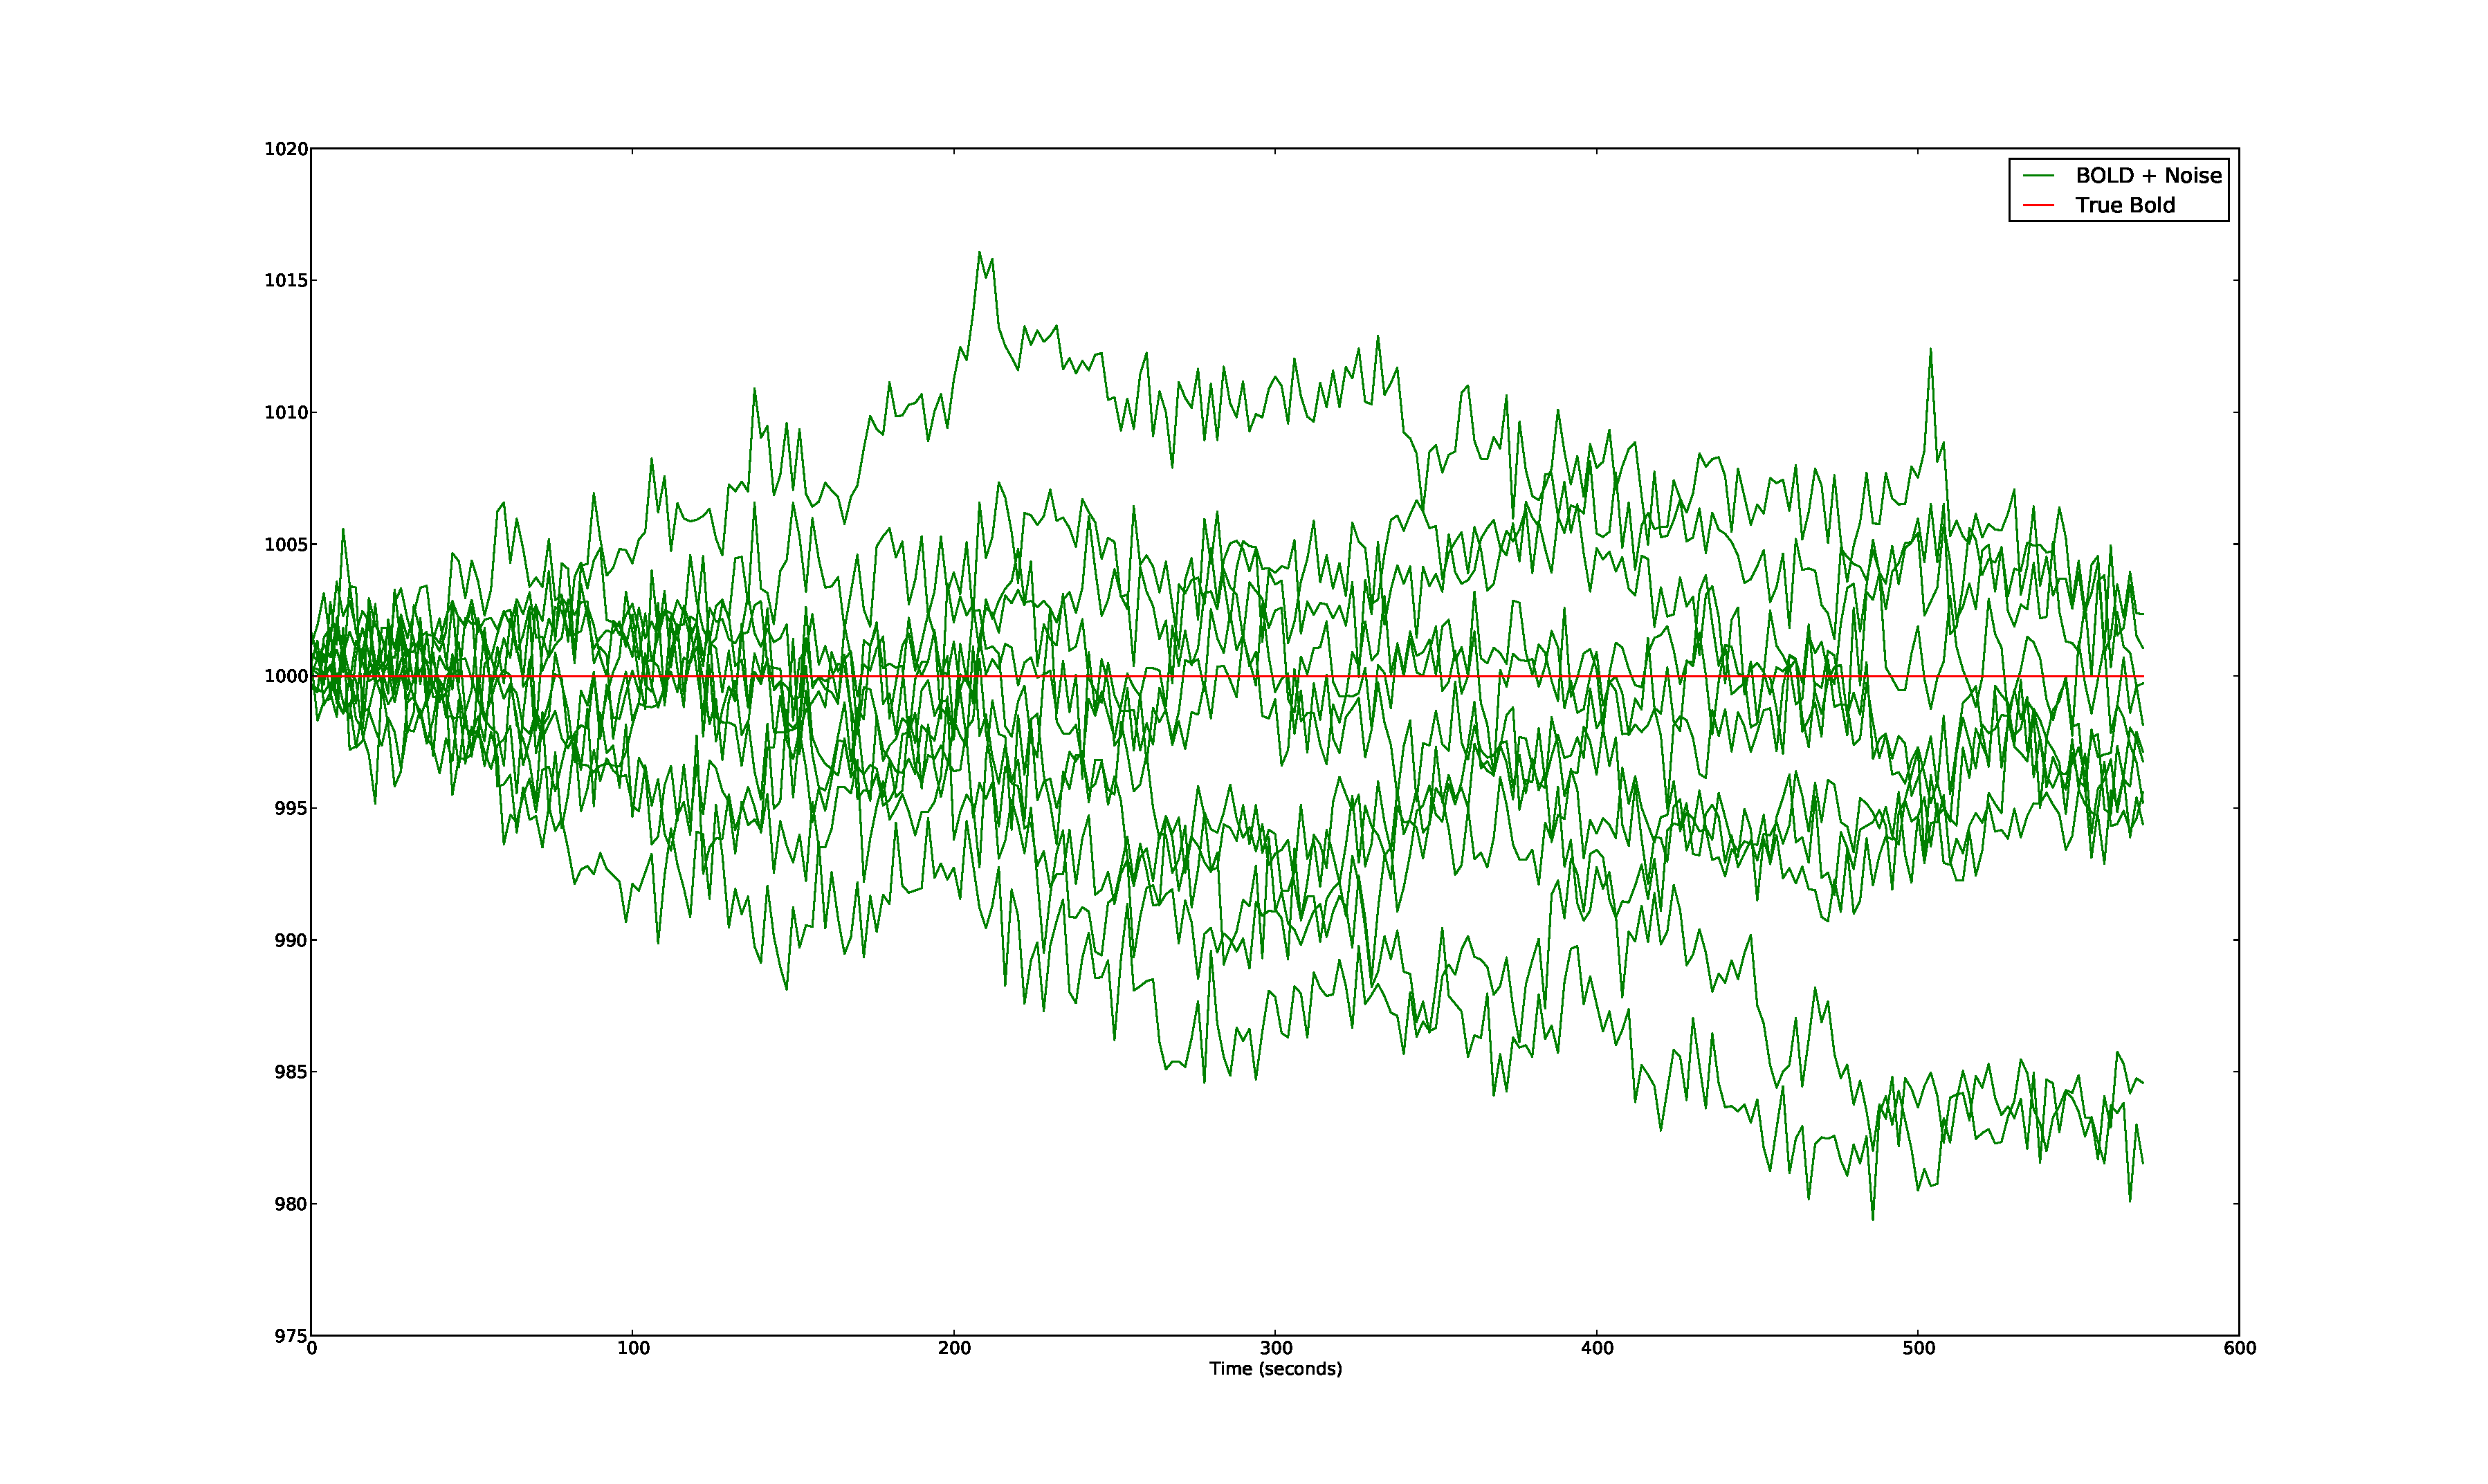
\includegraphics[clip=true,trim=6cm 3cm 6cm 3cm,height=7cm]{images/realization_noiseonly}
%\caption{Time-series lacking any real signal. With, ($\sigma_x = 0.01, \sigma_y=0.005$).}
%\label{fig:NoiseOnly}
%\end{figure}

\begin{figure}[H]
\centering
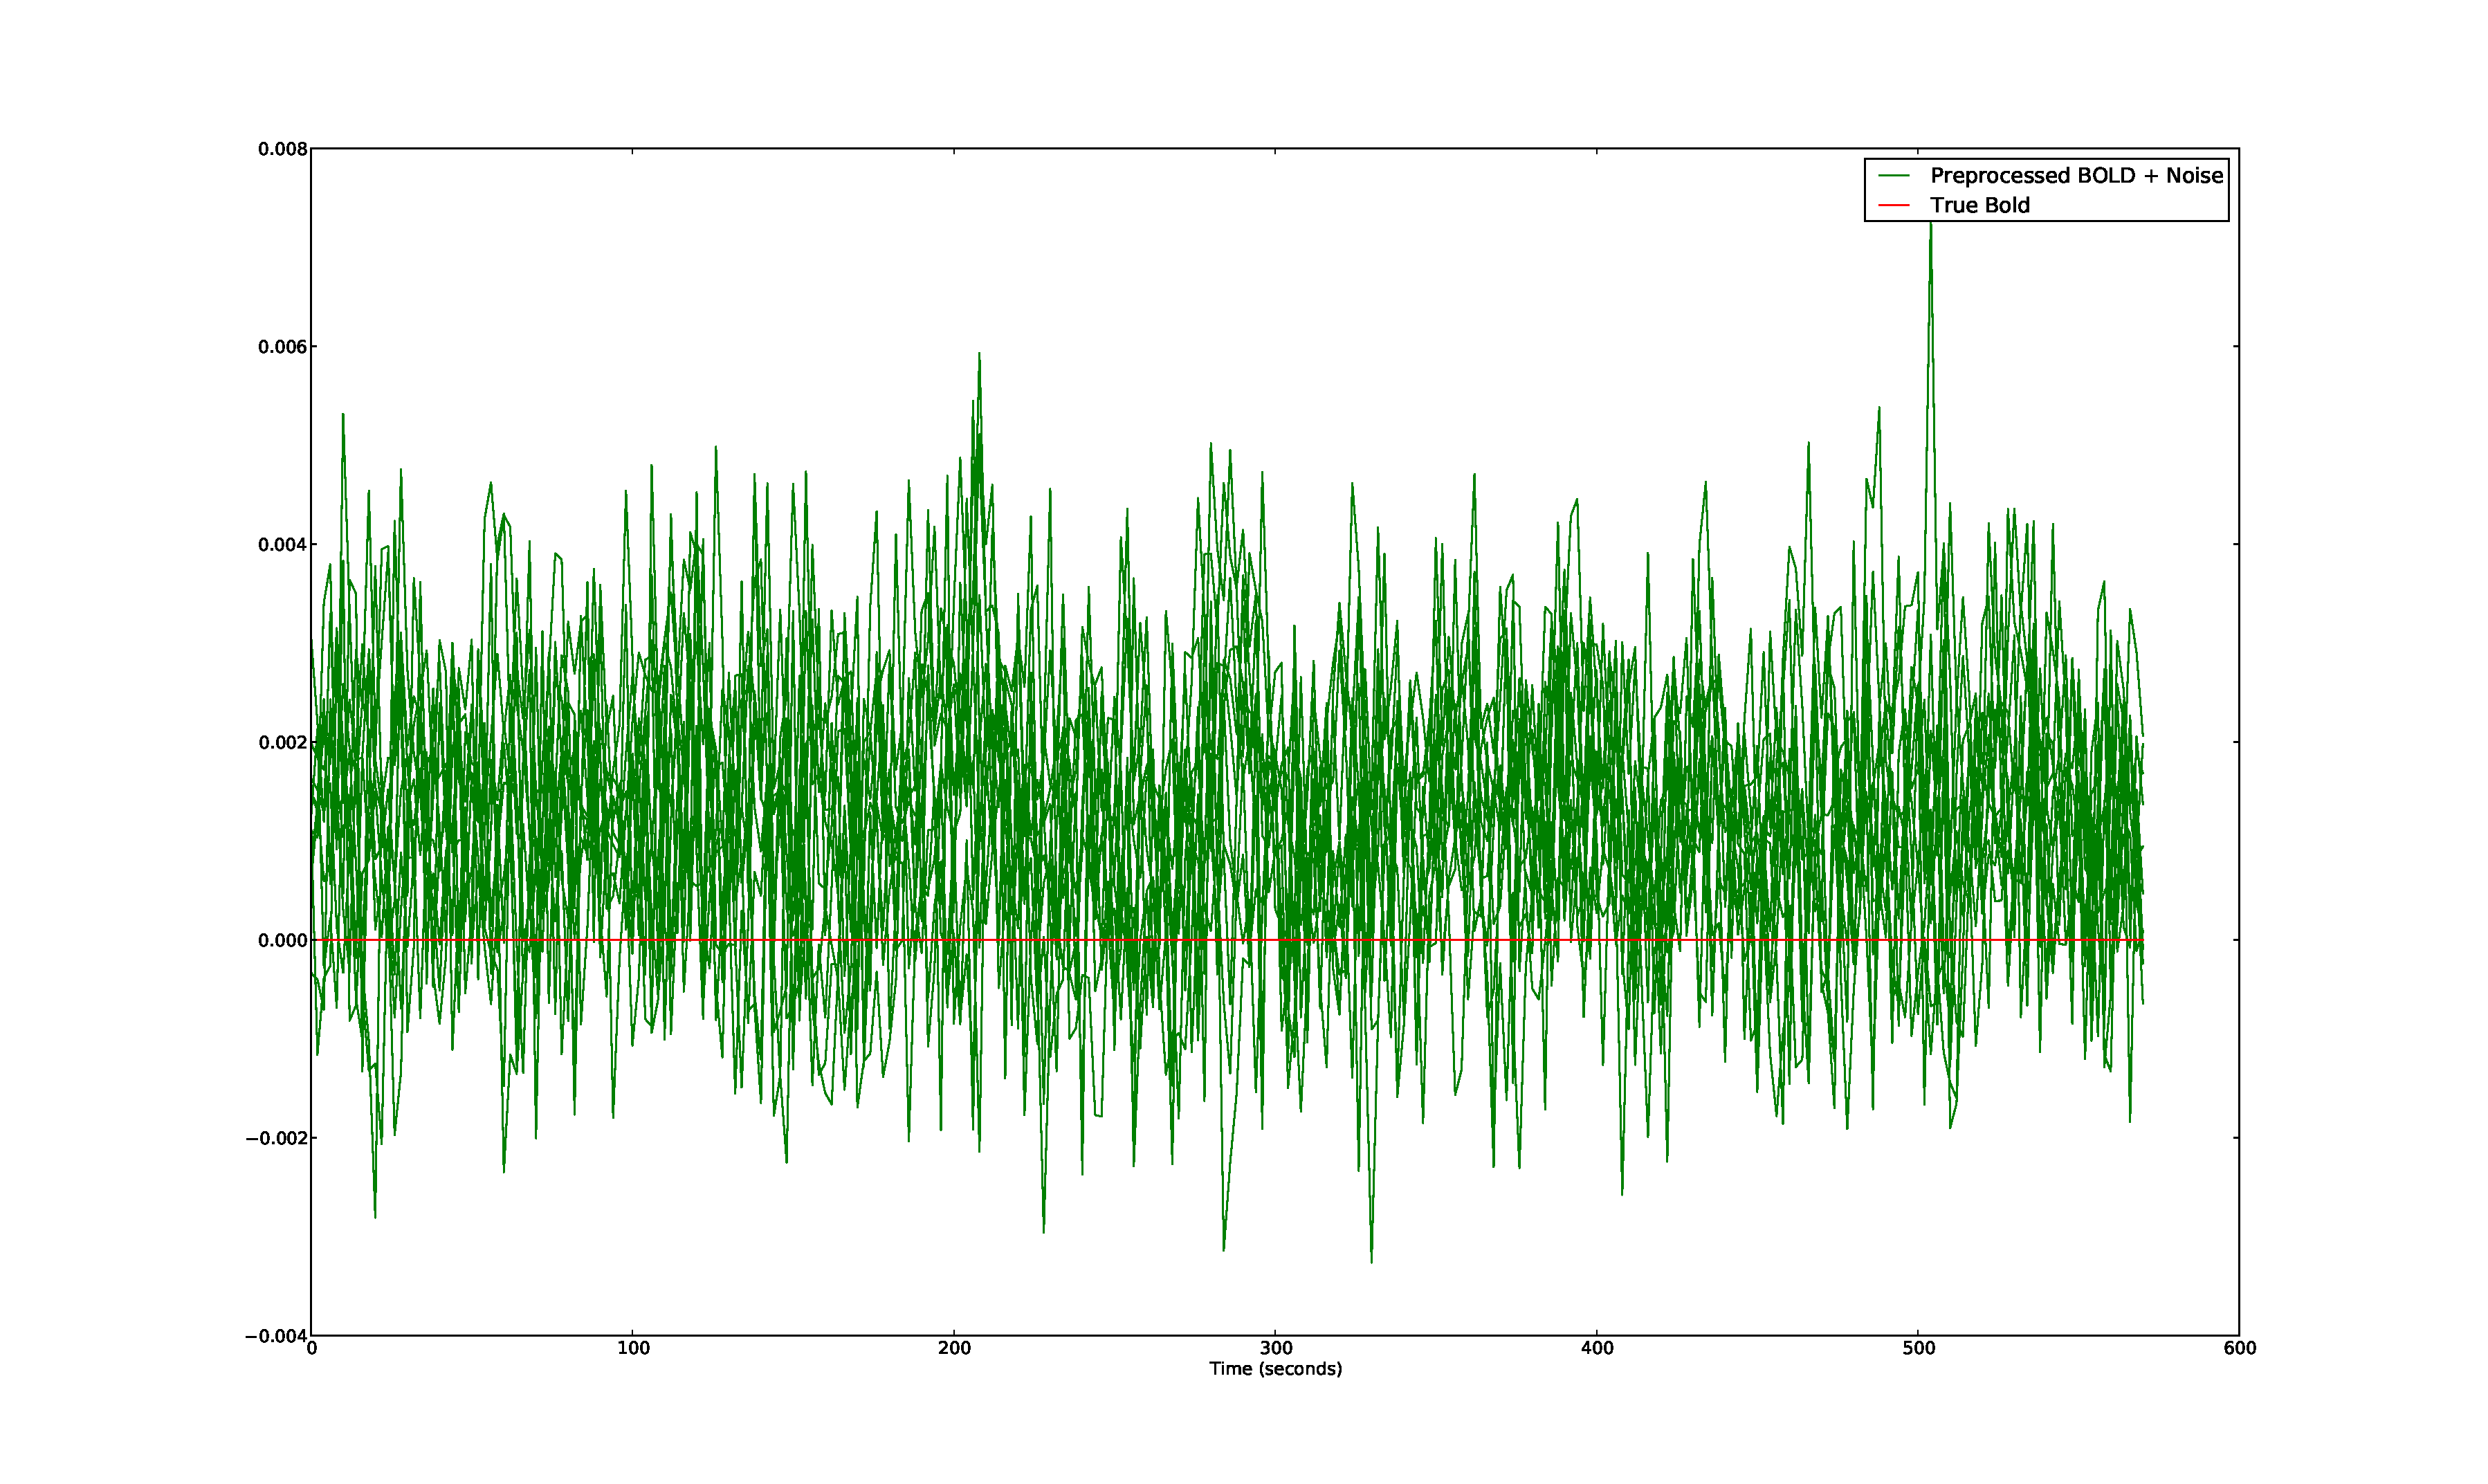
\includegraphics[clip=true,trim=6cm 2cm 6cm 3.5cm,width=15cm]{images/preprocessed_noiseonly}
\caption{Comparison of the preprocessed signals for the low noise signal-free case (
$\sigma_y = 0.01, \sigma_x = 0.005$).}
\label{fig:PreprocessedNoiseOnly}
\end{figure}

\begin{table}[t]
\centering
\begin{tabular}{|c | c | c | c | c | c | c | c | c |}
\hline 
$\tau_0$ & $\alpha$ & $E_0$    & $V_0$    & $\tau_s$ & $\tau_f$ & $\epsilon$  &  Residual   \\
\hline 
1.0324 & 0.33211 & 0.34058 & 0.03012 & 1.40665 & 2.52079 & 0.5311 &   0.00167  \\
 0.98189 & 0.33047 & 0.3386 & 0.03014 & 1.45707 & 2.47232 & 0.45049 & 0.00159   \\
 1.0429 & 0.33224 & 0.34124 & 0.02946 & 1.4618 & 2.49245 & 0.43012 &  0.00165   \\
 1.02054 & 0.3321 & 0.33484 & 0.02586 & 1.45848 & 2.48741 & 0.4193 &  0.00151   \\
 1.0565 & 0.33405 & 0.33758 & 0.02791 & 1.43784 & 2.52545 & 0.47517 & 0.00152   \\
 1.01867 & 0.33528 & 0.33918 & 0.02782 & 1.48345 & 2.49605 & 0.44209 &0.00156   \\
 1.051 & 0.33038 & 0.33837 & 0.02985 & 1.47651 & 2.48621 & 0.42719 &  0.00159   \\
 1.00281 & 0.32929 & 0.33988 & 0.0298 & 1.43519 & 2.49256 & 0.48899 & 0.00164   \\
 1.00893 & 0.33273 & 0.33982 & 0.0289 & 1.42903 & 2.49754 & 0.45688 & 0.00168   \\
 1.01289 & 0.33275 & 0.3376 & 0.02997 & 1.41188 & 2.49881 & 0.50628 & 0.00183   \\
 1.10247 & 0.33371 & 0.3419 & 0.02939 & 1.43774 & 2.53384 & 0.44079 & 0.00195   \\
\hline                                                                  
1.03009 & 0.33228 & 0.33905 & 0.02902 & 1.44506 & 2.50031 & 0.46076 & 0.00165 \\
\hline
\end{tabular}
\caption{Estimated Parameters on 11 different runs with low noise and no signal present.}
\label{tab:NoiseOnlyResults} 
\end{table}

\begin{figure}[H]
\centering
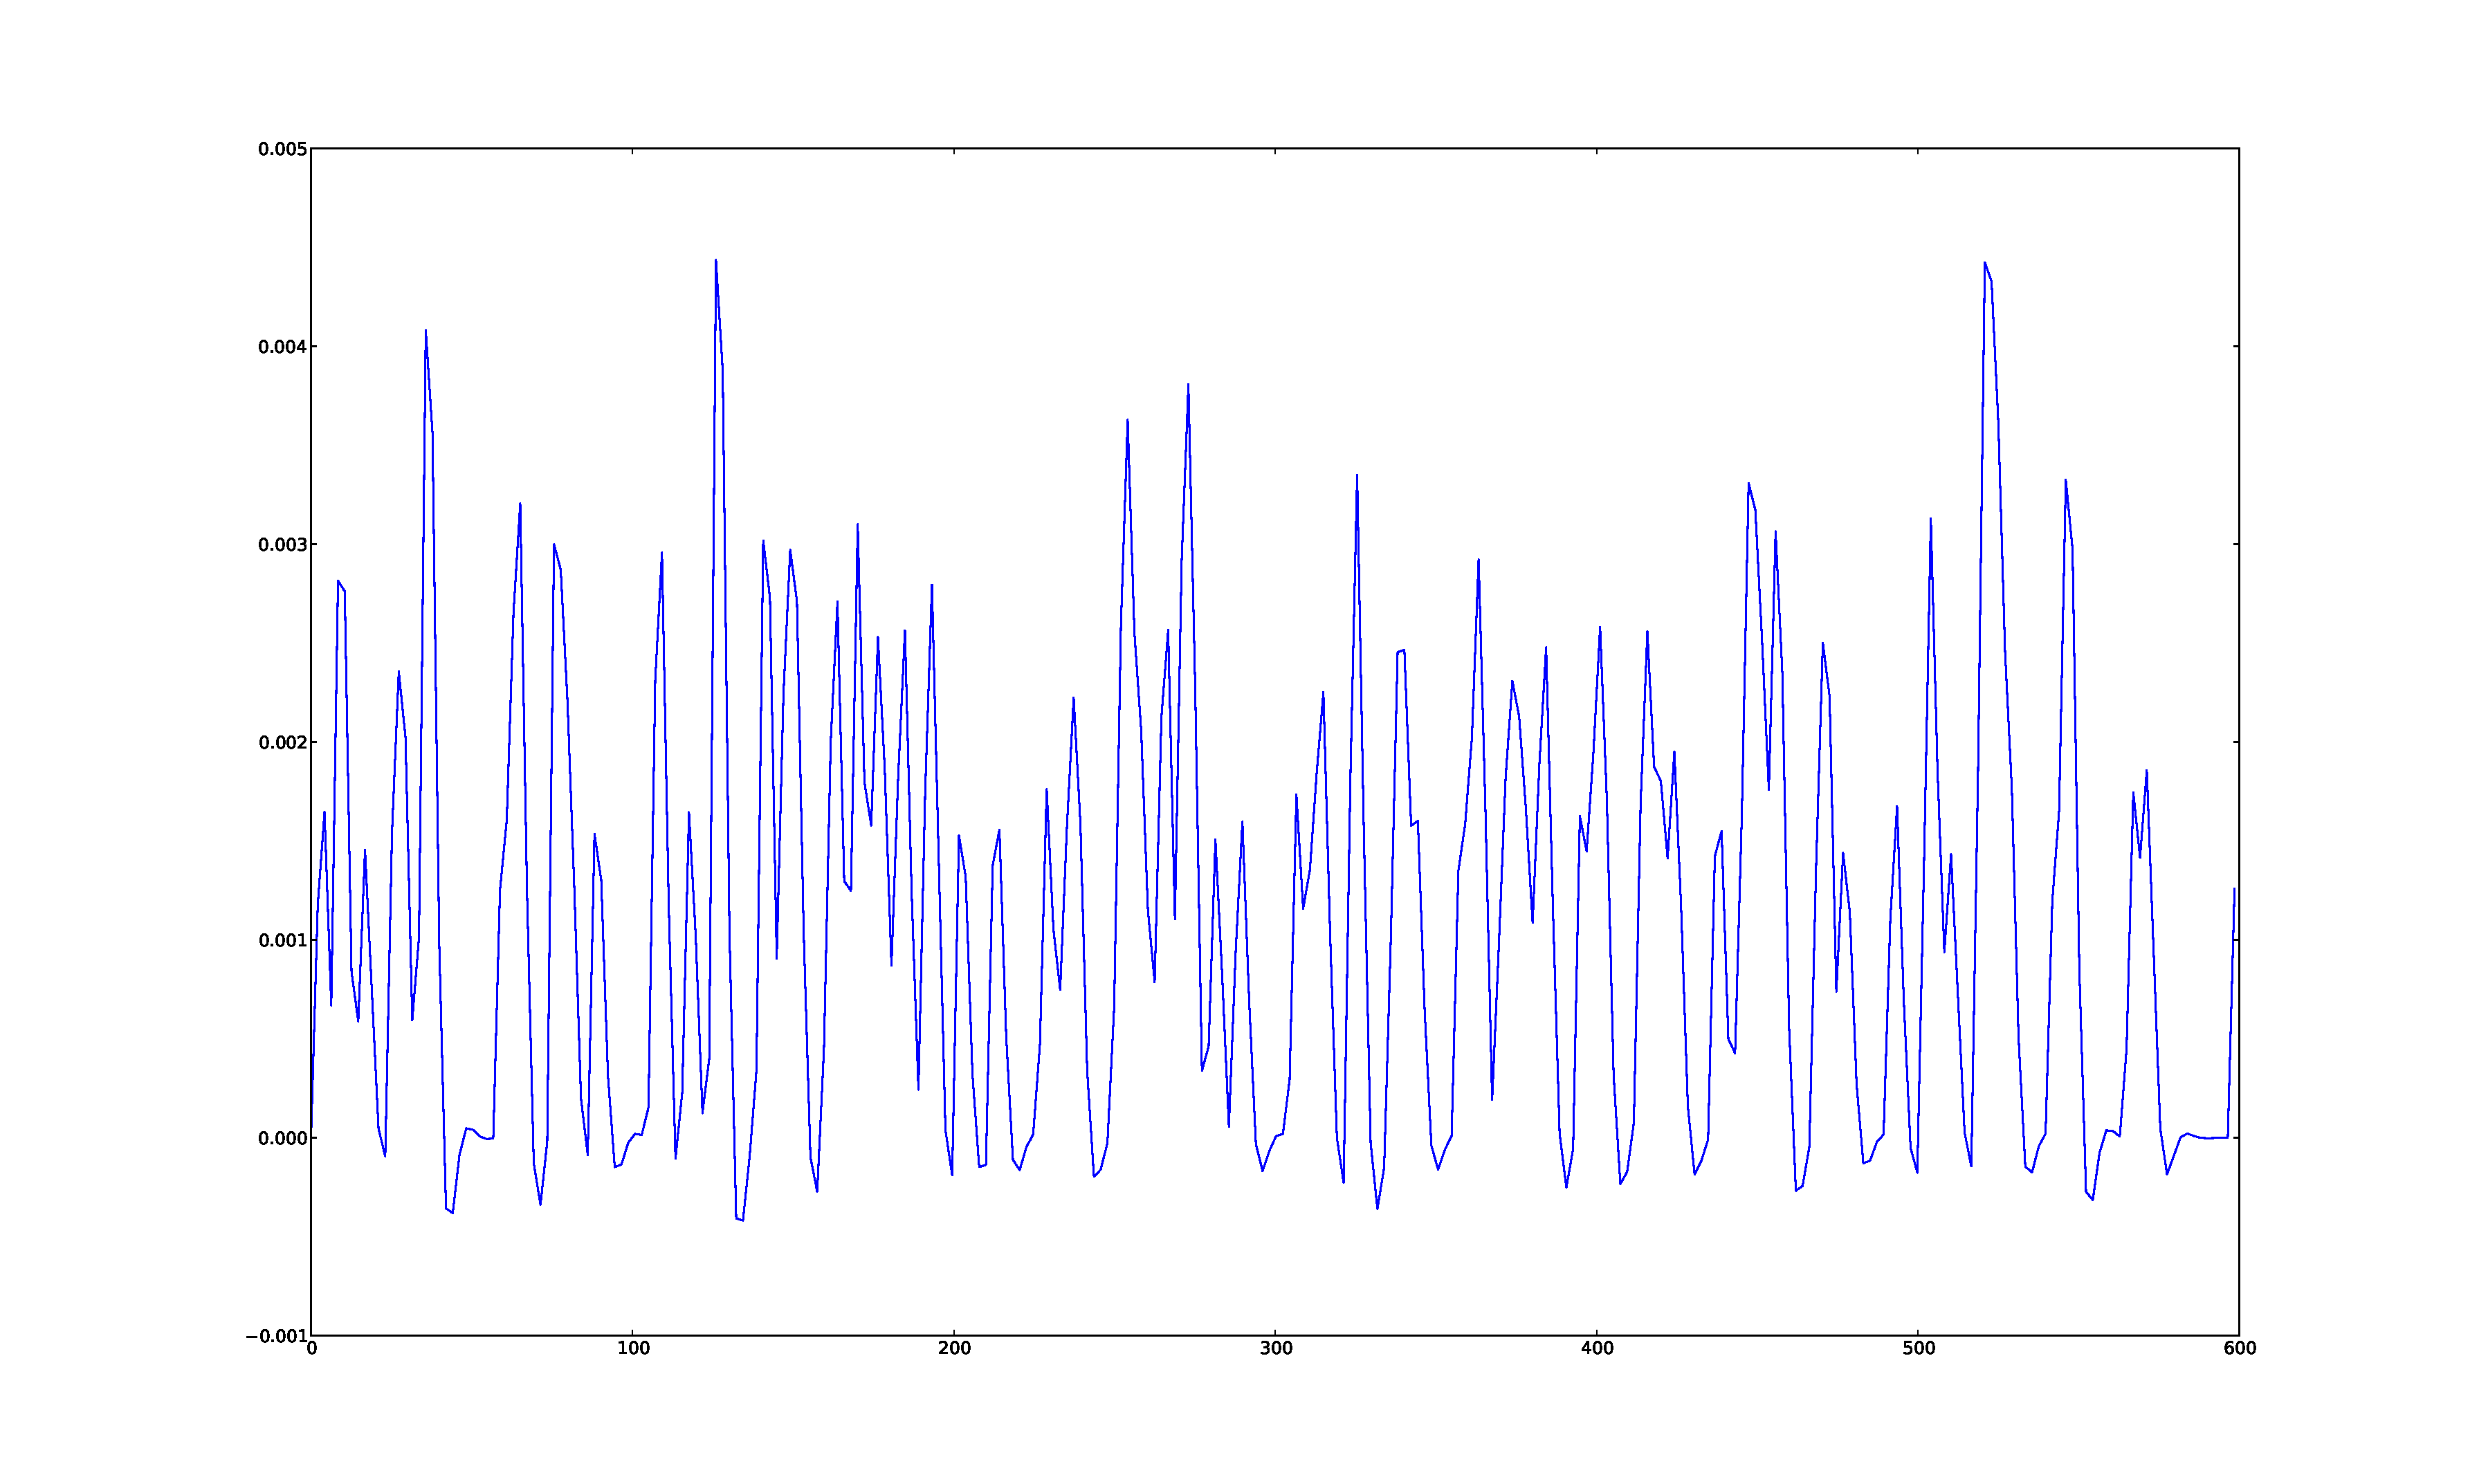
\includegraphics[clip=true,trim=6cm 3cm 6cm 3cm,height=9cm]{images/fits_noiseonly}
\caption{Fits to the non-active, low noise signal. Note that the line is thick because all
the estimates overlap. All 11 fitted lines.}
\label{fig:fits_noiseonly}
\end{figure}

\begin{figure}[H]
\centering
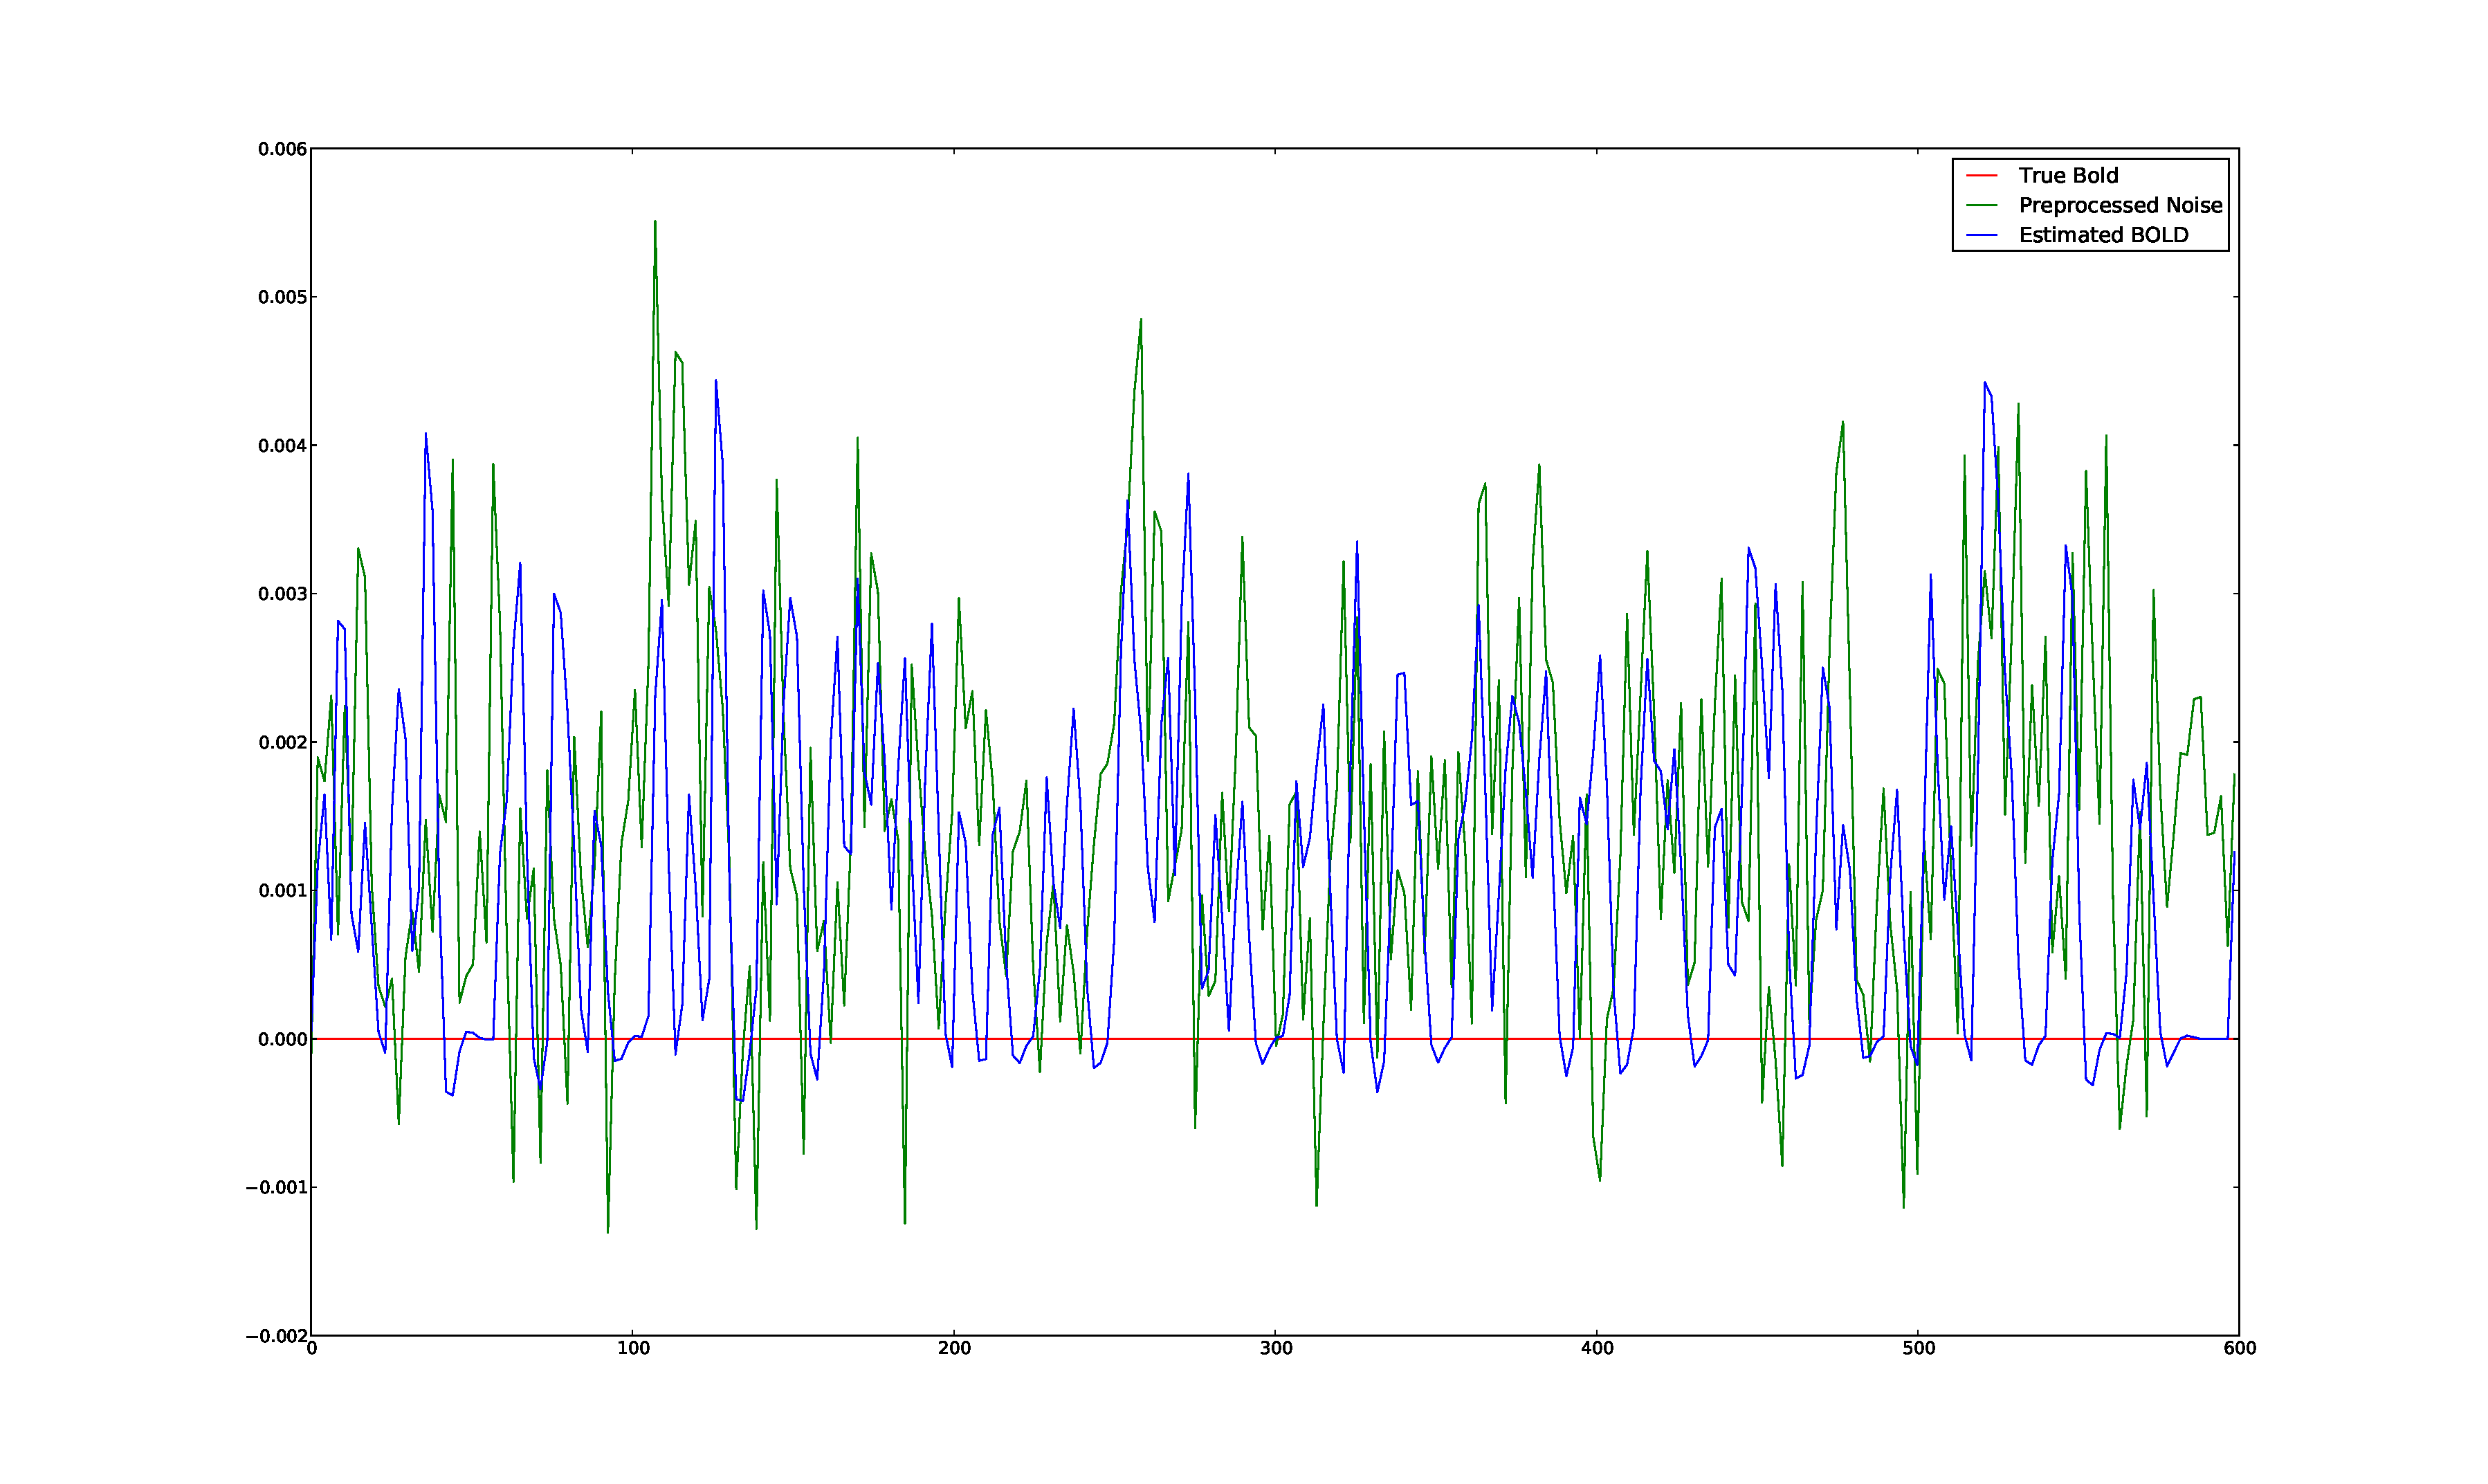
\includegraphics[clip=true,trim=6cm 3cm 6cm 3cm,height=9cm]{images/justnoise_fit_0}
\caption{Fit from a single particle filter run, with the noise input. }
\label{fig:justnoise_fit_0}
\end{figure} %uses allnoise/ALLNOISE-0-w0

\begin{figure}[H]
\centering
\subfigure[$\tau_0$, $\alpha$, $E_0$, $V_0$]
{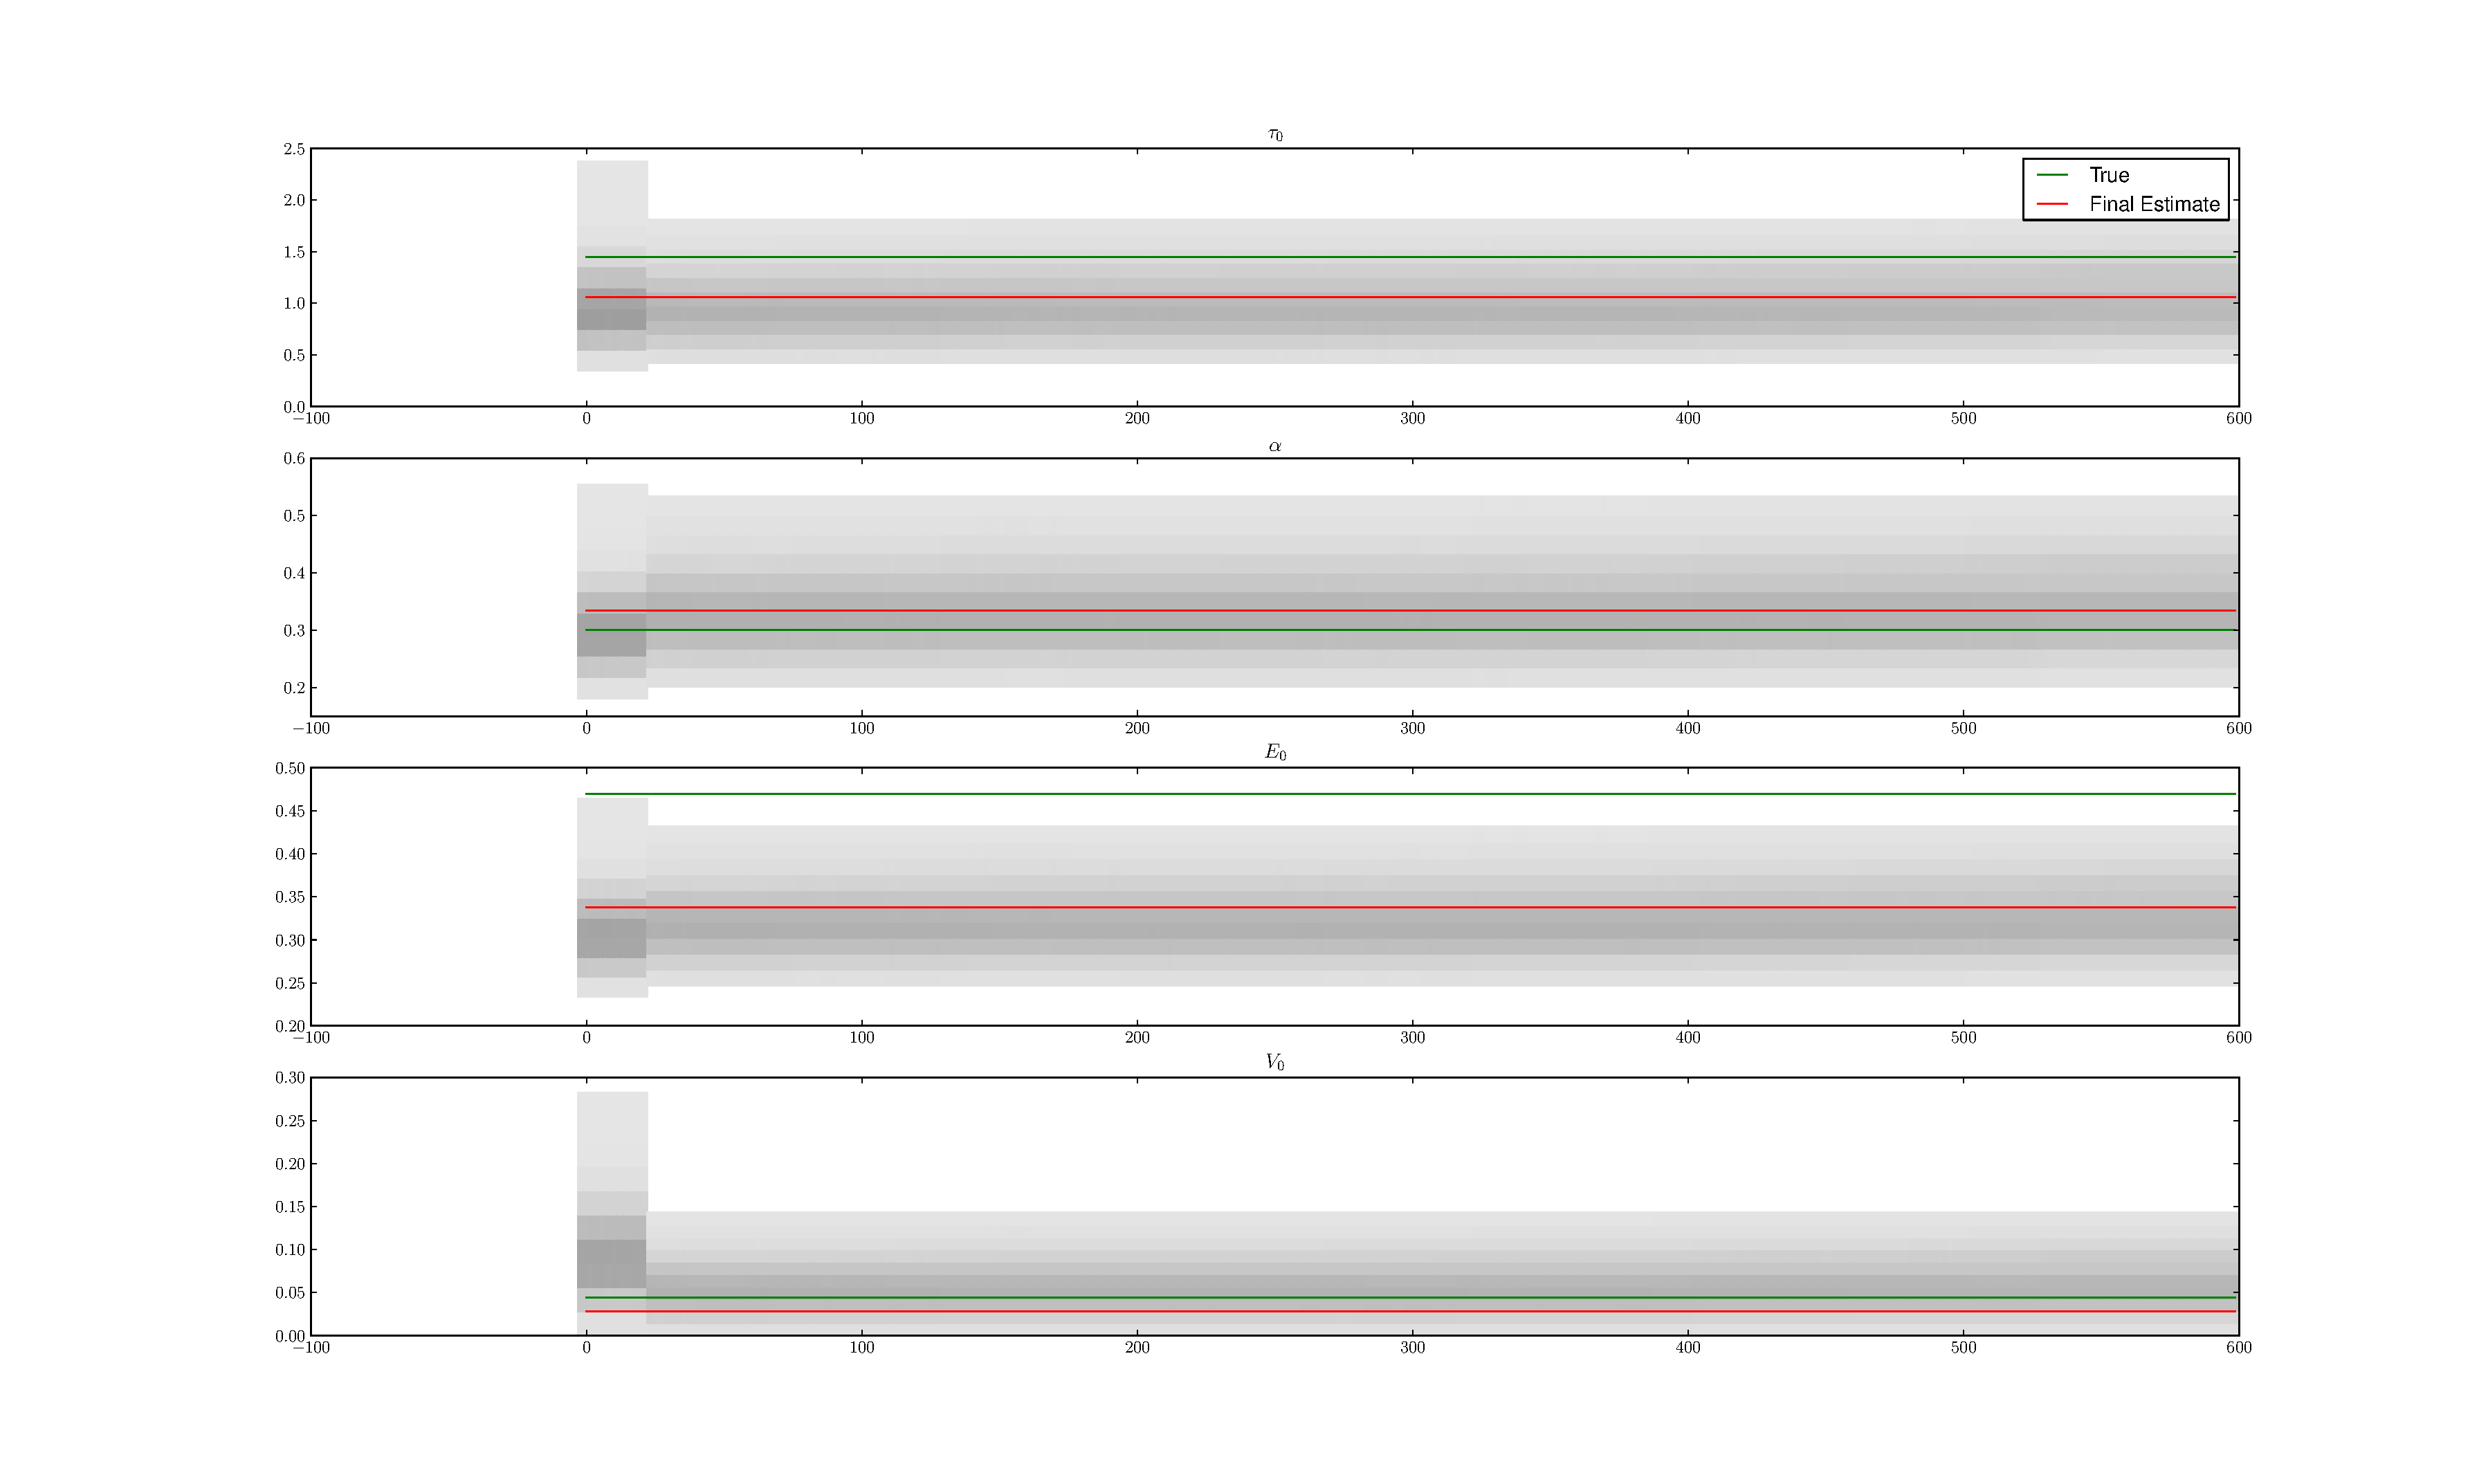
\includegraphics[clip=true,trim=6cm 2cm 6cm 3cm, height=9cm]{images/justnoise_hist_1}}\\
\end{figure}

\begin{figure}[H]
\centering
\subfigure[$\tau_s$, $\tau_f$, $\epsilon$, $v$] 
{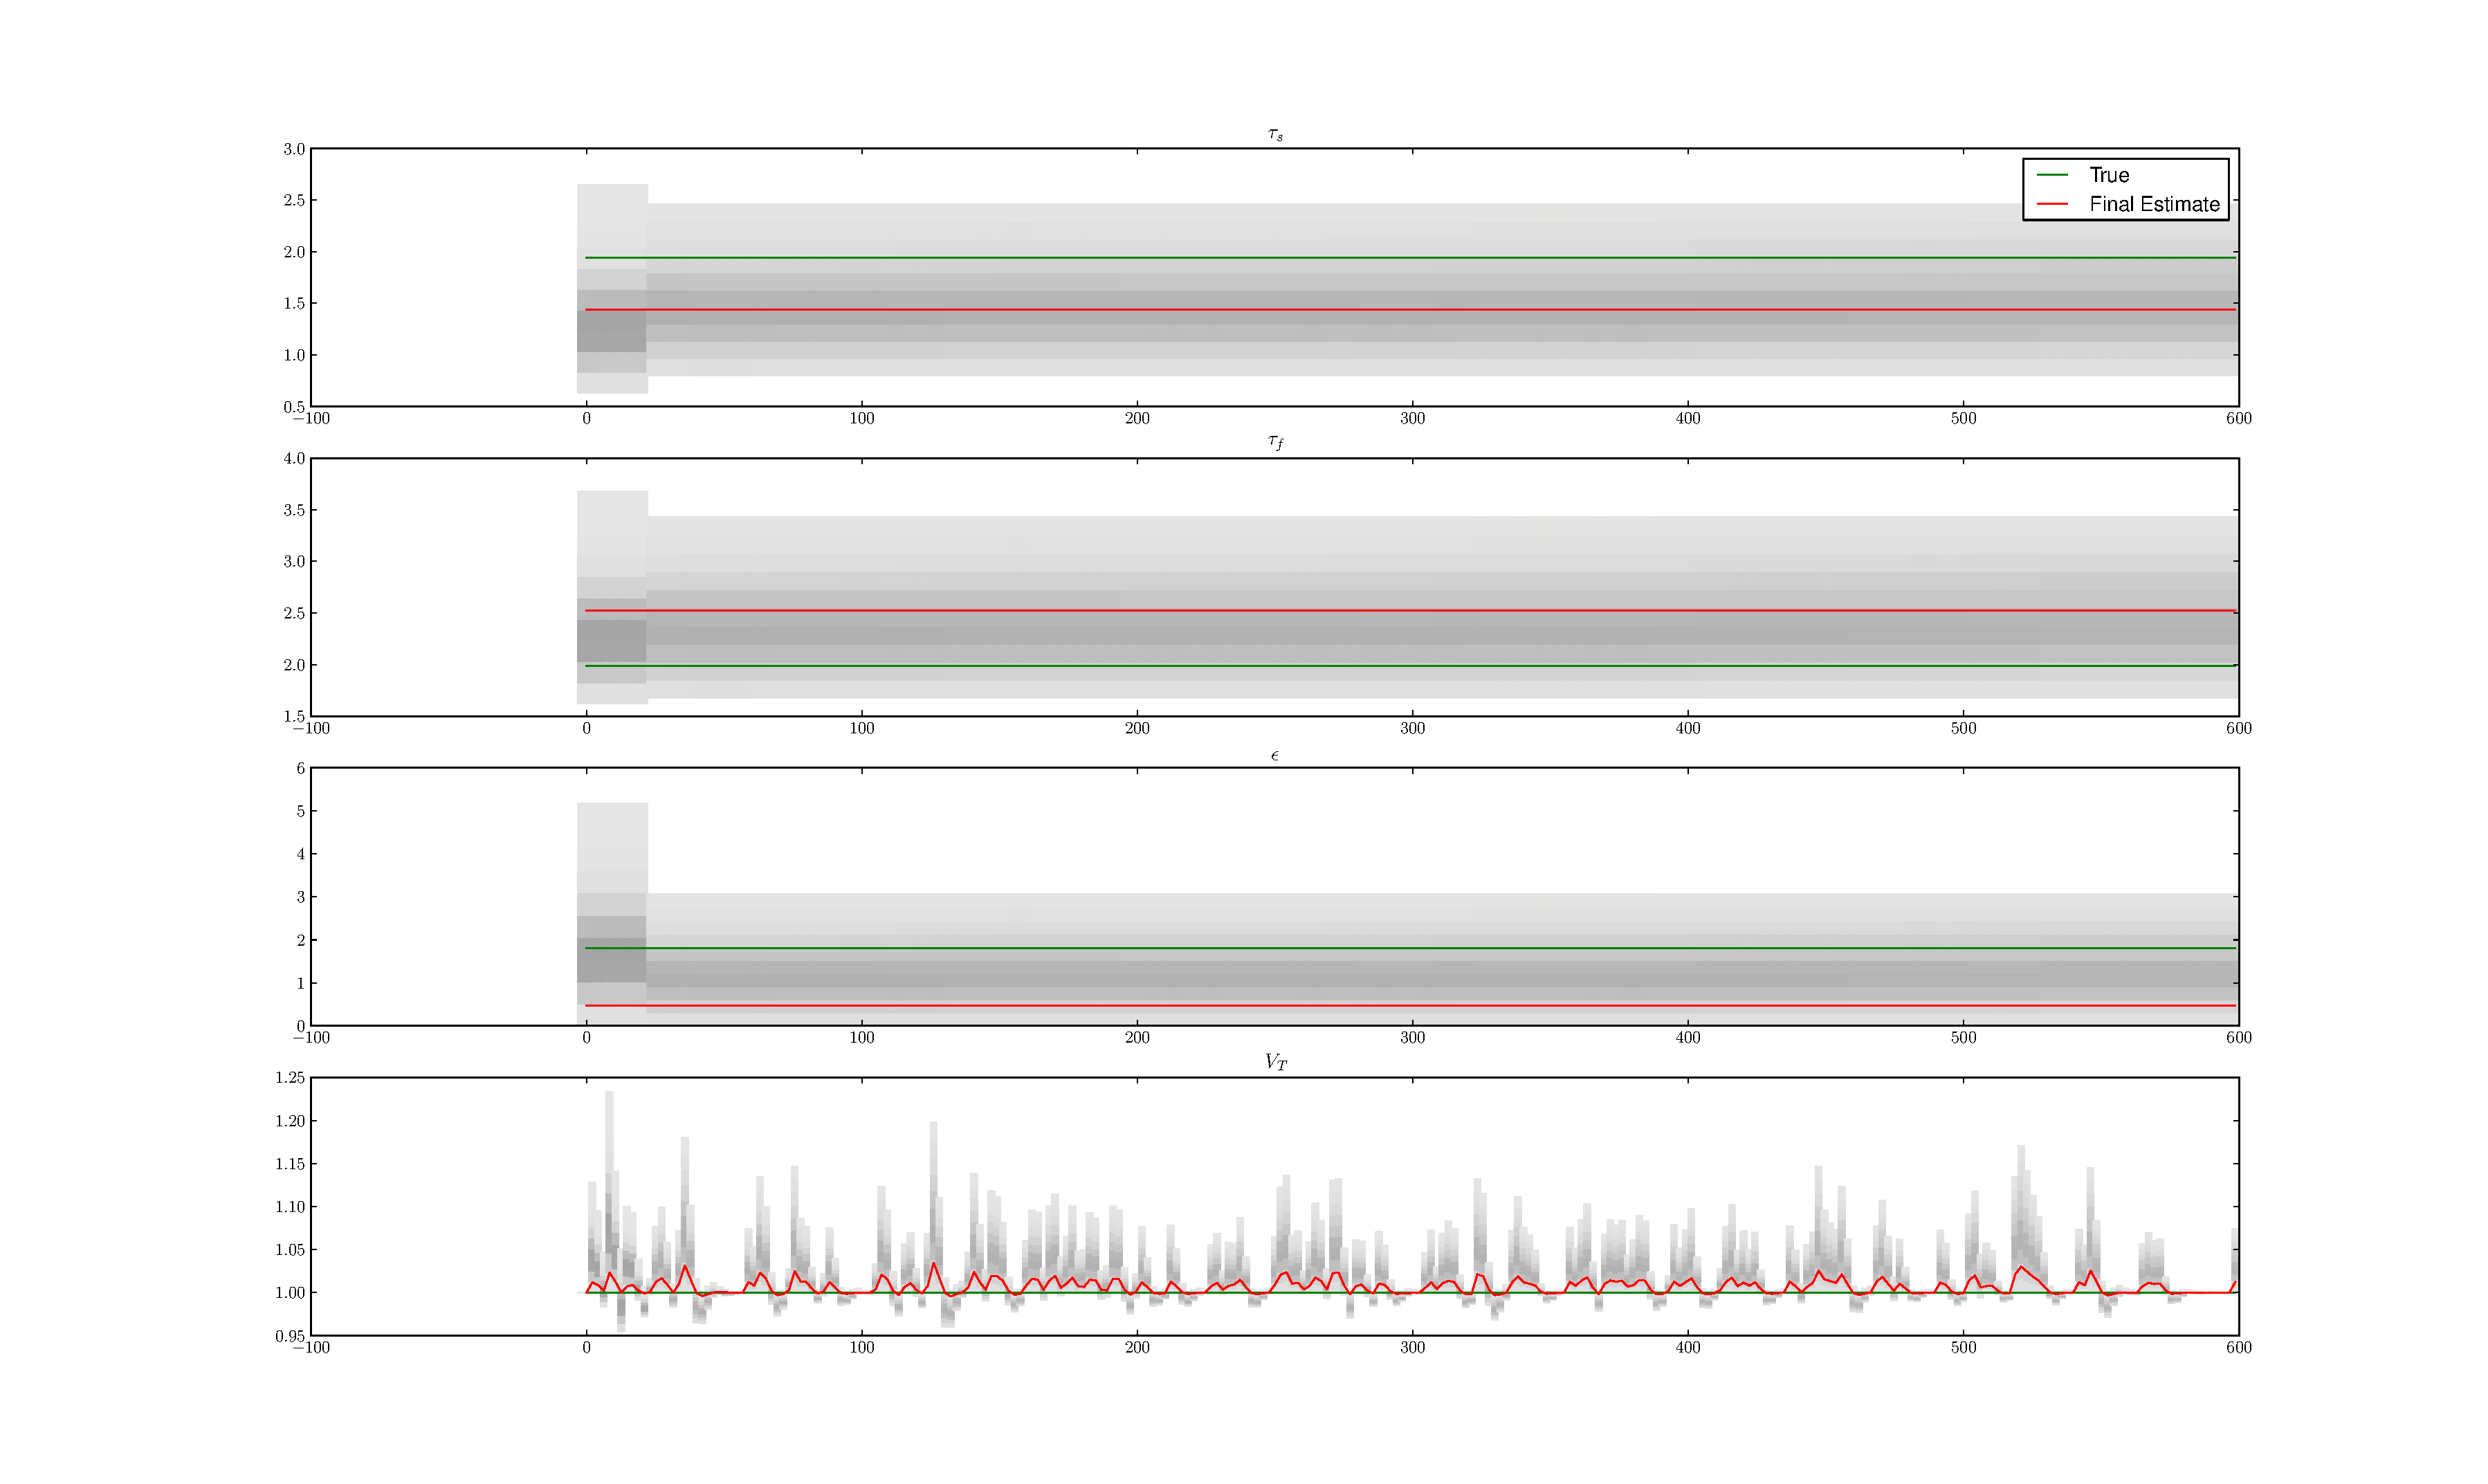
\includegraphics[clip=true,trim=6cm 2cm 6cm 3cm, height=9cm]{images/justnoise_hist_2}}\\
\end{figure}

\begin{figure}[H]
\centering
\subfigure[$q$, $s$, $f$, $BOLD$ ]
{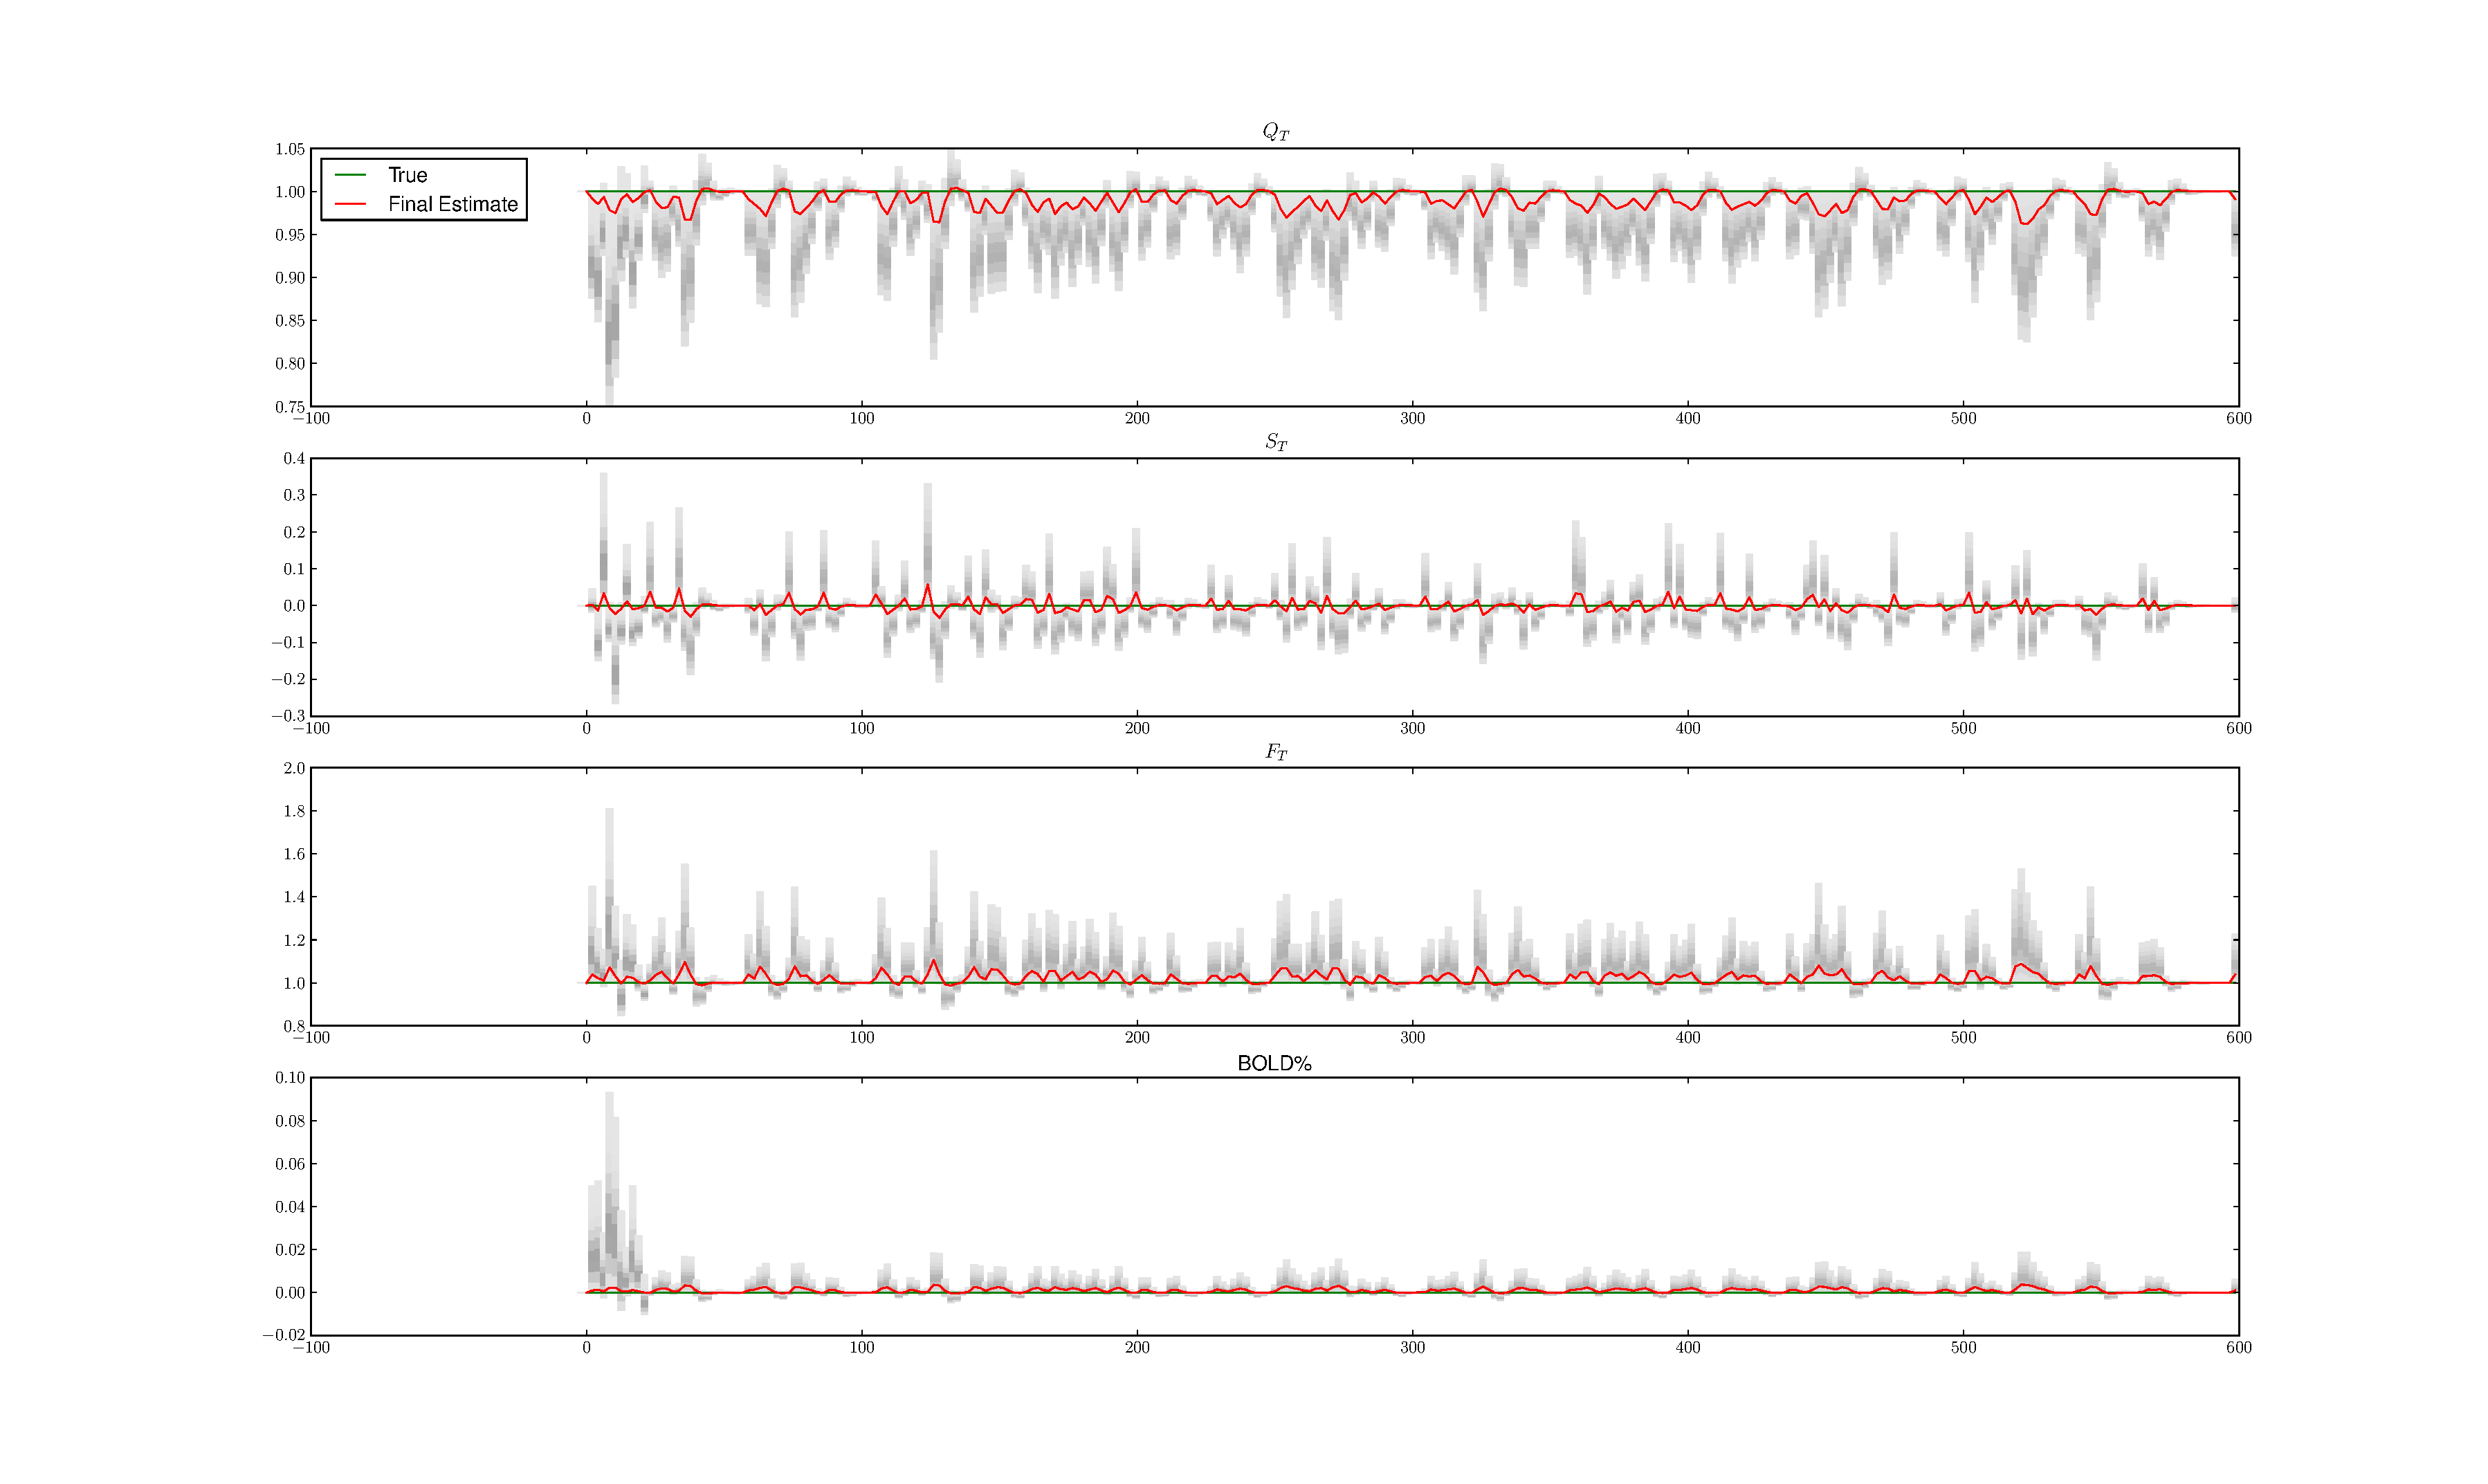
\includegraphics[clip=true,trim=6cm 2cm 6cm 3cm, height=9cm]{images/justnoise_hist_3}}
\caption{Converging histogram for parameters when the signal consists purely of low level noise. 
Same run as \autoref{fig:justnoise_fit_0}}
\label{fig:JustNoiseConvergence}
\end{figure}

The data shows that the parameters did really not converge
\autoref{fig:JustNoiseConvergence}.
The peaks never even reached 1\% difference
(\autoref{fig:PreprocessedNoiseOnly}) so  the signal  stayed 
well within the range of $0.005$, the standard deviation of the weighting function.
Note that the residuals
were actually lower than the residuals in the low noise simulation from \autoref{sec:SimLowNoise}
and the parameter estimates were extremely consistent across 11 runs. 
The low residual was caused by the overall
signal being significantly smaller than any previous simulation.
From these results it would seem that lack of convergence could be
a differentiating factor from a signal with an actual signal; however,
the next section casts doubt on this possibility. 

%NO SIGNAL, VERY HIGH NOISE
\subsection{Pure Noise, High Magnitude}
\label{sec:PureNoiseHighMag}
To determine how the particle filter responds to active, yet unrelated
portions of the brain, this section repeats the test of \autoref{sec:PureNoiseLowMag} 
with much higher noise peaks. To simulate this case another
pure noise signal was generated using $\sigma_x$ of $0.1$ and $\sigma_y$ of $0.05$.

As before, the convergence all follows a similar path, leaving almost no
variance in the estimated time series (\autoref{fig:fits_noiseonly_high}). 
Interestingly the algorithm suffered from almost constant particle deprivation, 
meaning that the heuristic
for rescuing the particle filter from particle deprivation, discussed in
\autoref{sec:Resampling}, in fact was working against the proper course of action. 
The proper course of action in this case would be for the particle filter to fail,
since no particle can really properly estimate a random sequence. When this mechanism
was removed, all 11 runs stopped due to particle deprivation (all weights hit zero). 
The problem with allowing particle deprivation to occur is that it can \emph{rarely}
occur in good data if the prior distribution does not cover a solution. 

Because of the preprocessing steps, the pure noise signal can look markedly like a real
signal (\autoref{fig:justbignoise_fit_0}). The preprocessing causes the particle filter
to converge to a non-zero response in spite of the fact that the input does not correlate
with the stimuli in any way (\autoref{fig:fits_noiseonly_high}). 

\begin{figure}[H]
\centering
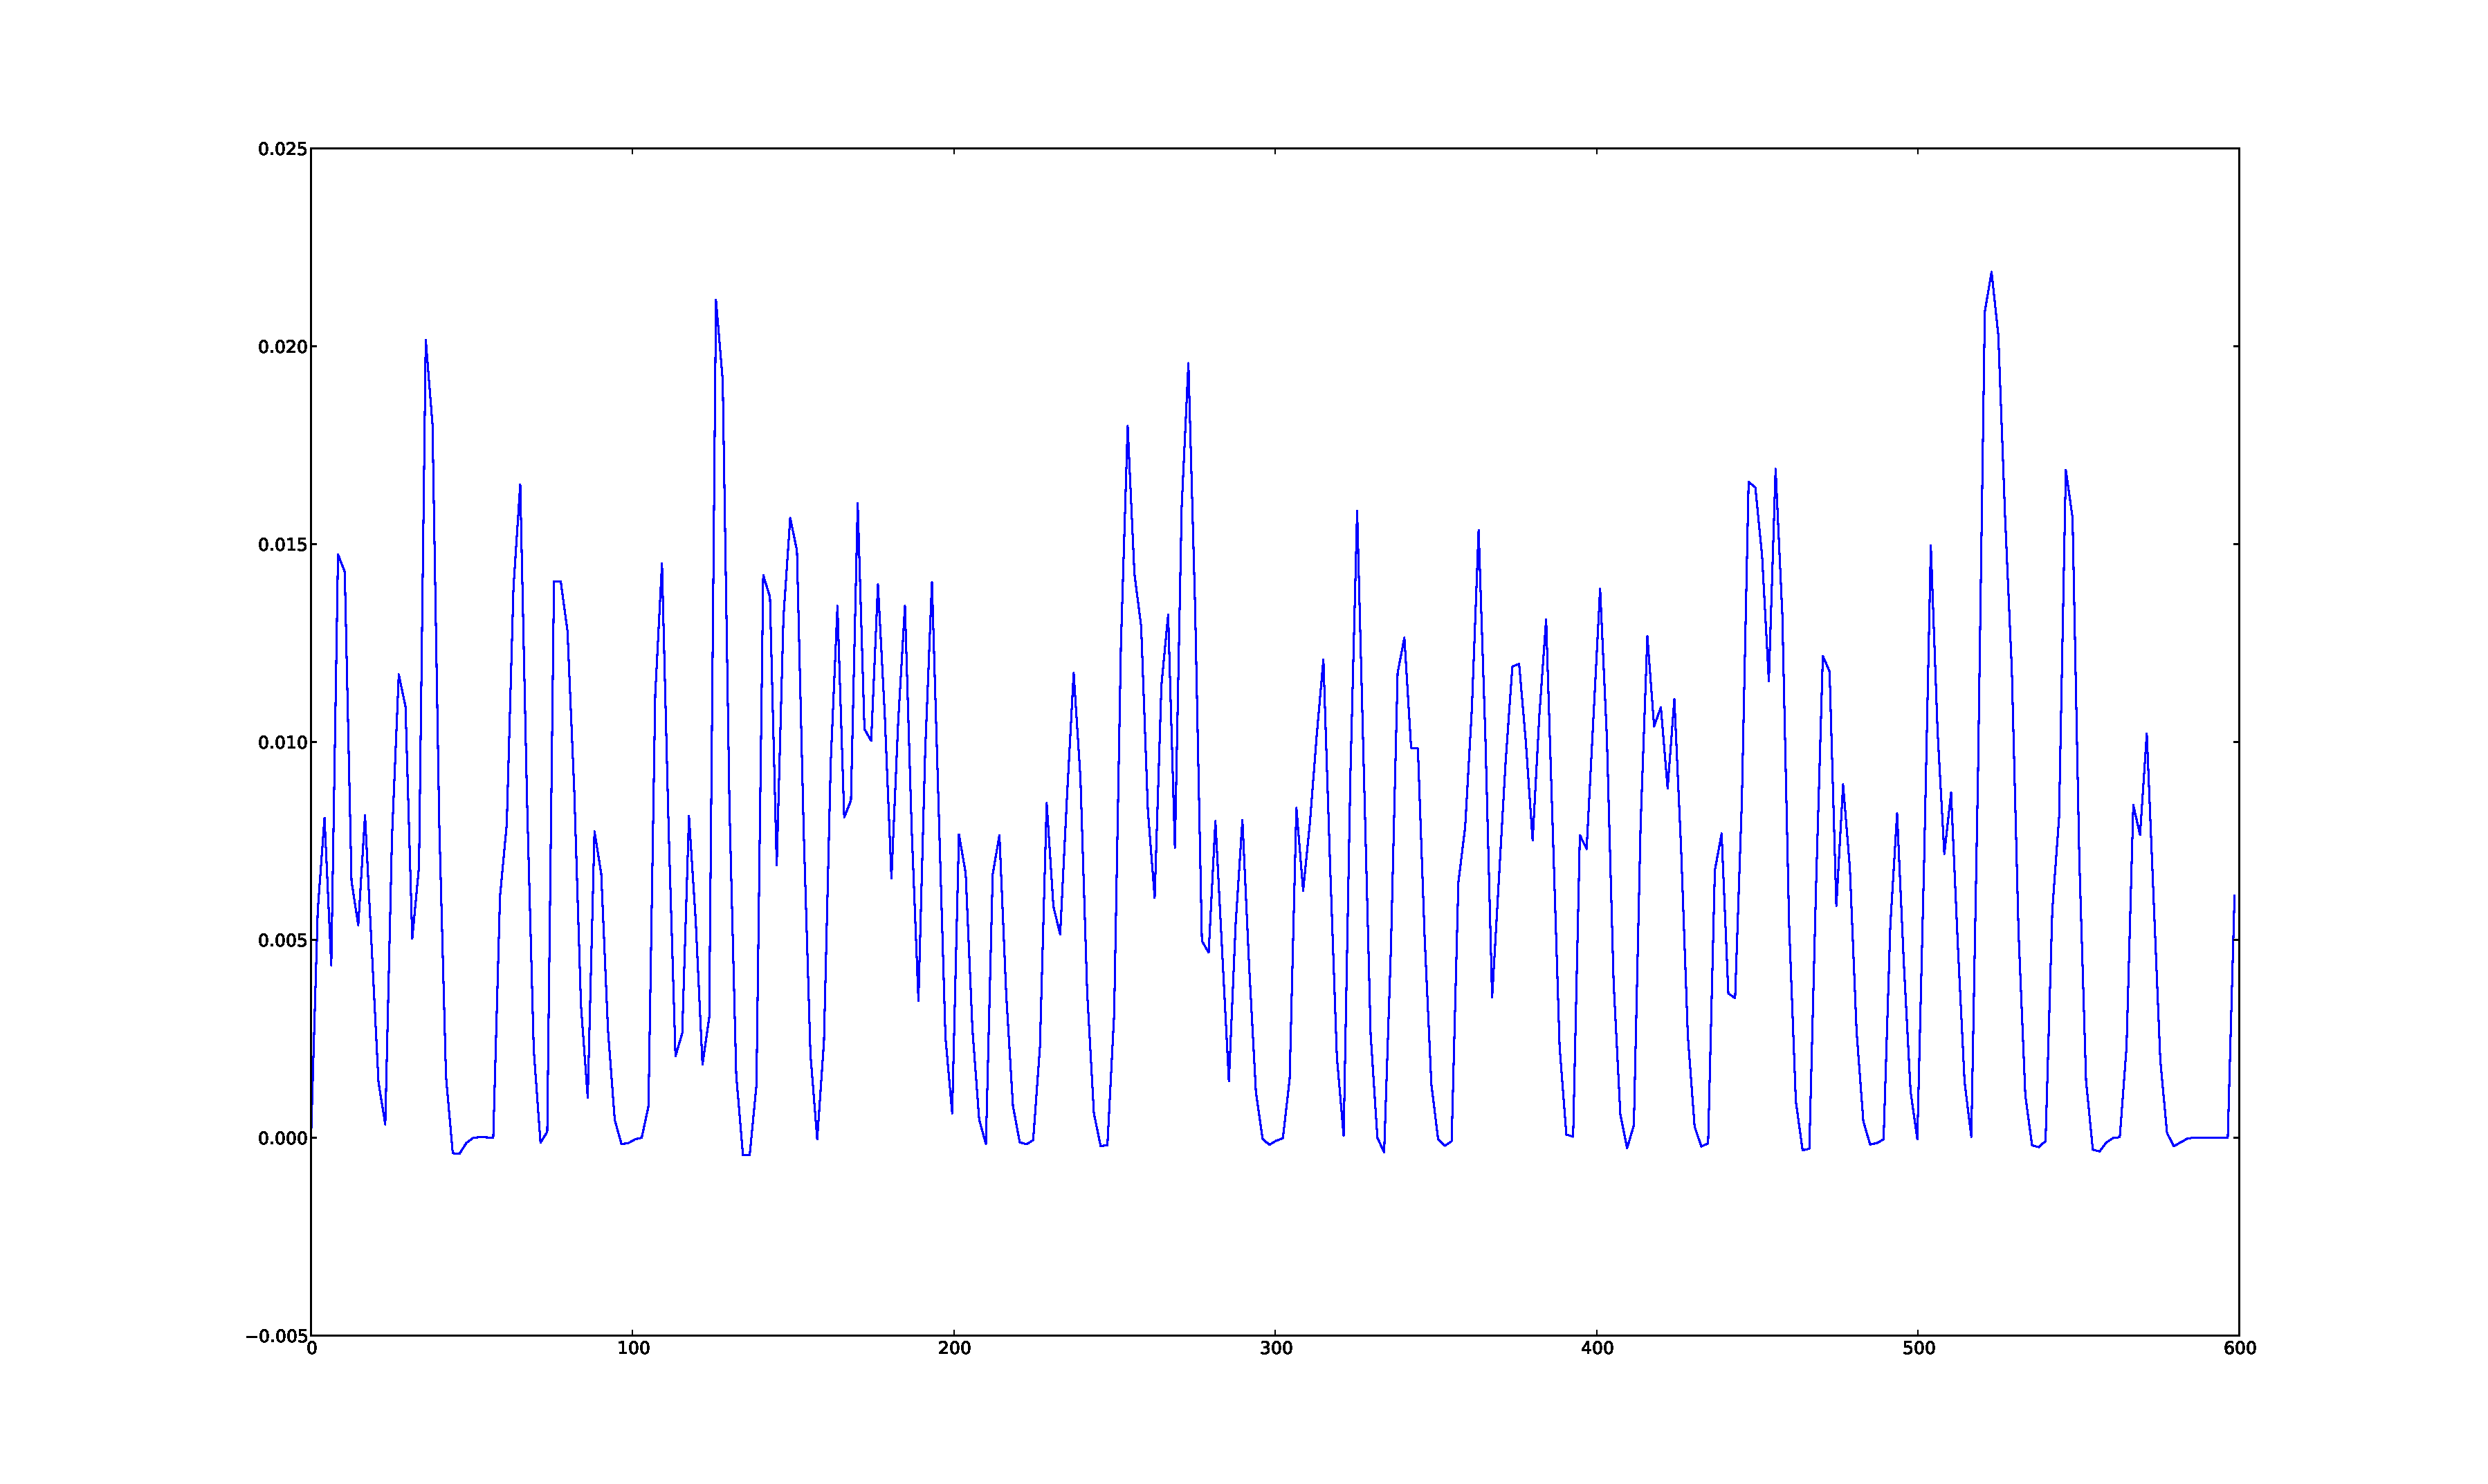
\includegraphics[clip=true,trim=6cm 2cm 5cm 3cm,width=15cm]{images/fits_noiseonly_high}
\caption{BOLD estimates for the non-active, high noise signal. Note the line thickness is caused
by all the estimates overlapping.}
\label{fig:fits_noiseonly_high}
\end{figure}

\begin{figure}[H]
\centering
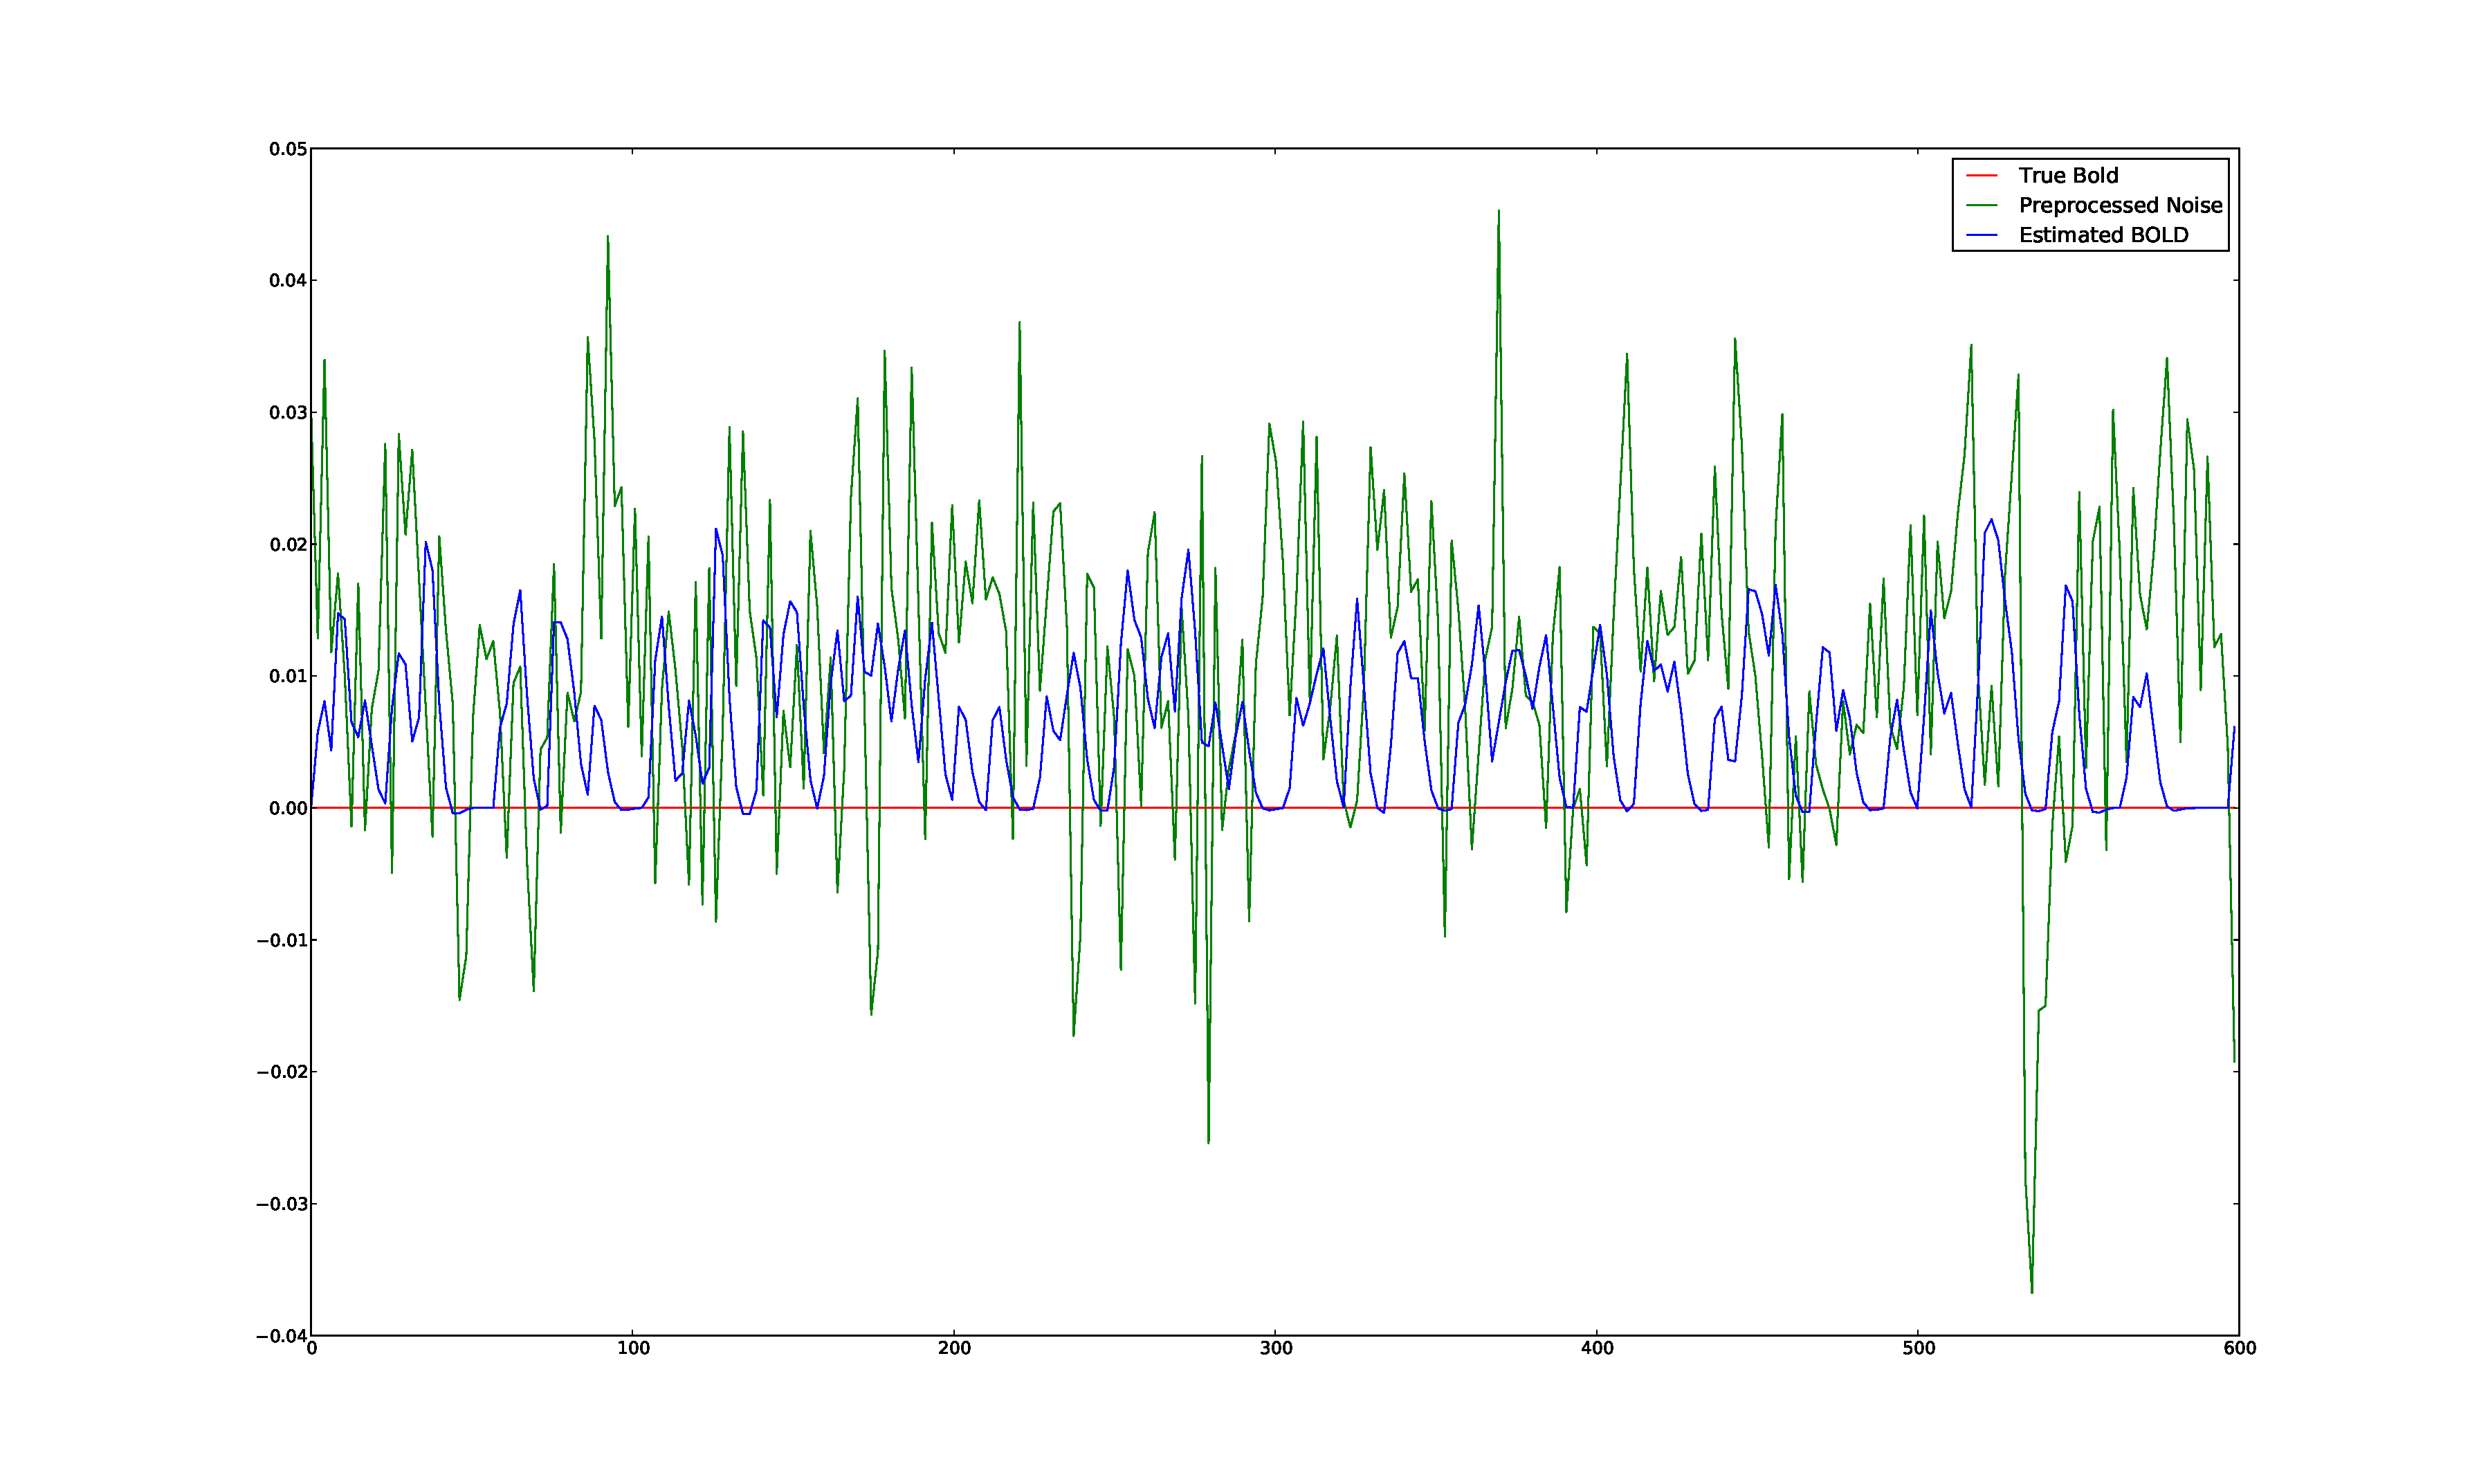
\includegraphics[clip=true,trim=6cm 3cm 6cm 3cm,height=9cm]{images/justbignoise_fit_0}
\caption{Fit from a single particle filter run, with the noise input. }
\label{fig:justbignoise_fit_0}
\end{figure} %uses allnoise/ALLNOISE-0-w0

%\begin{figure}[H]
%\centering
%\subfigure[$\tau_0$, $\alpha$, $E_0$, $V_0$]
%{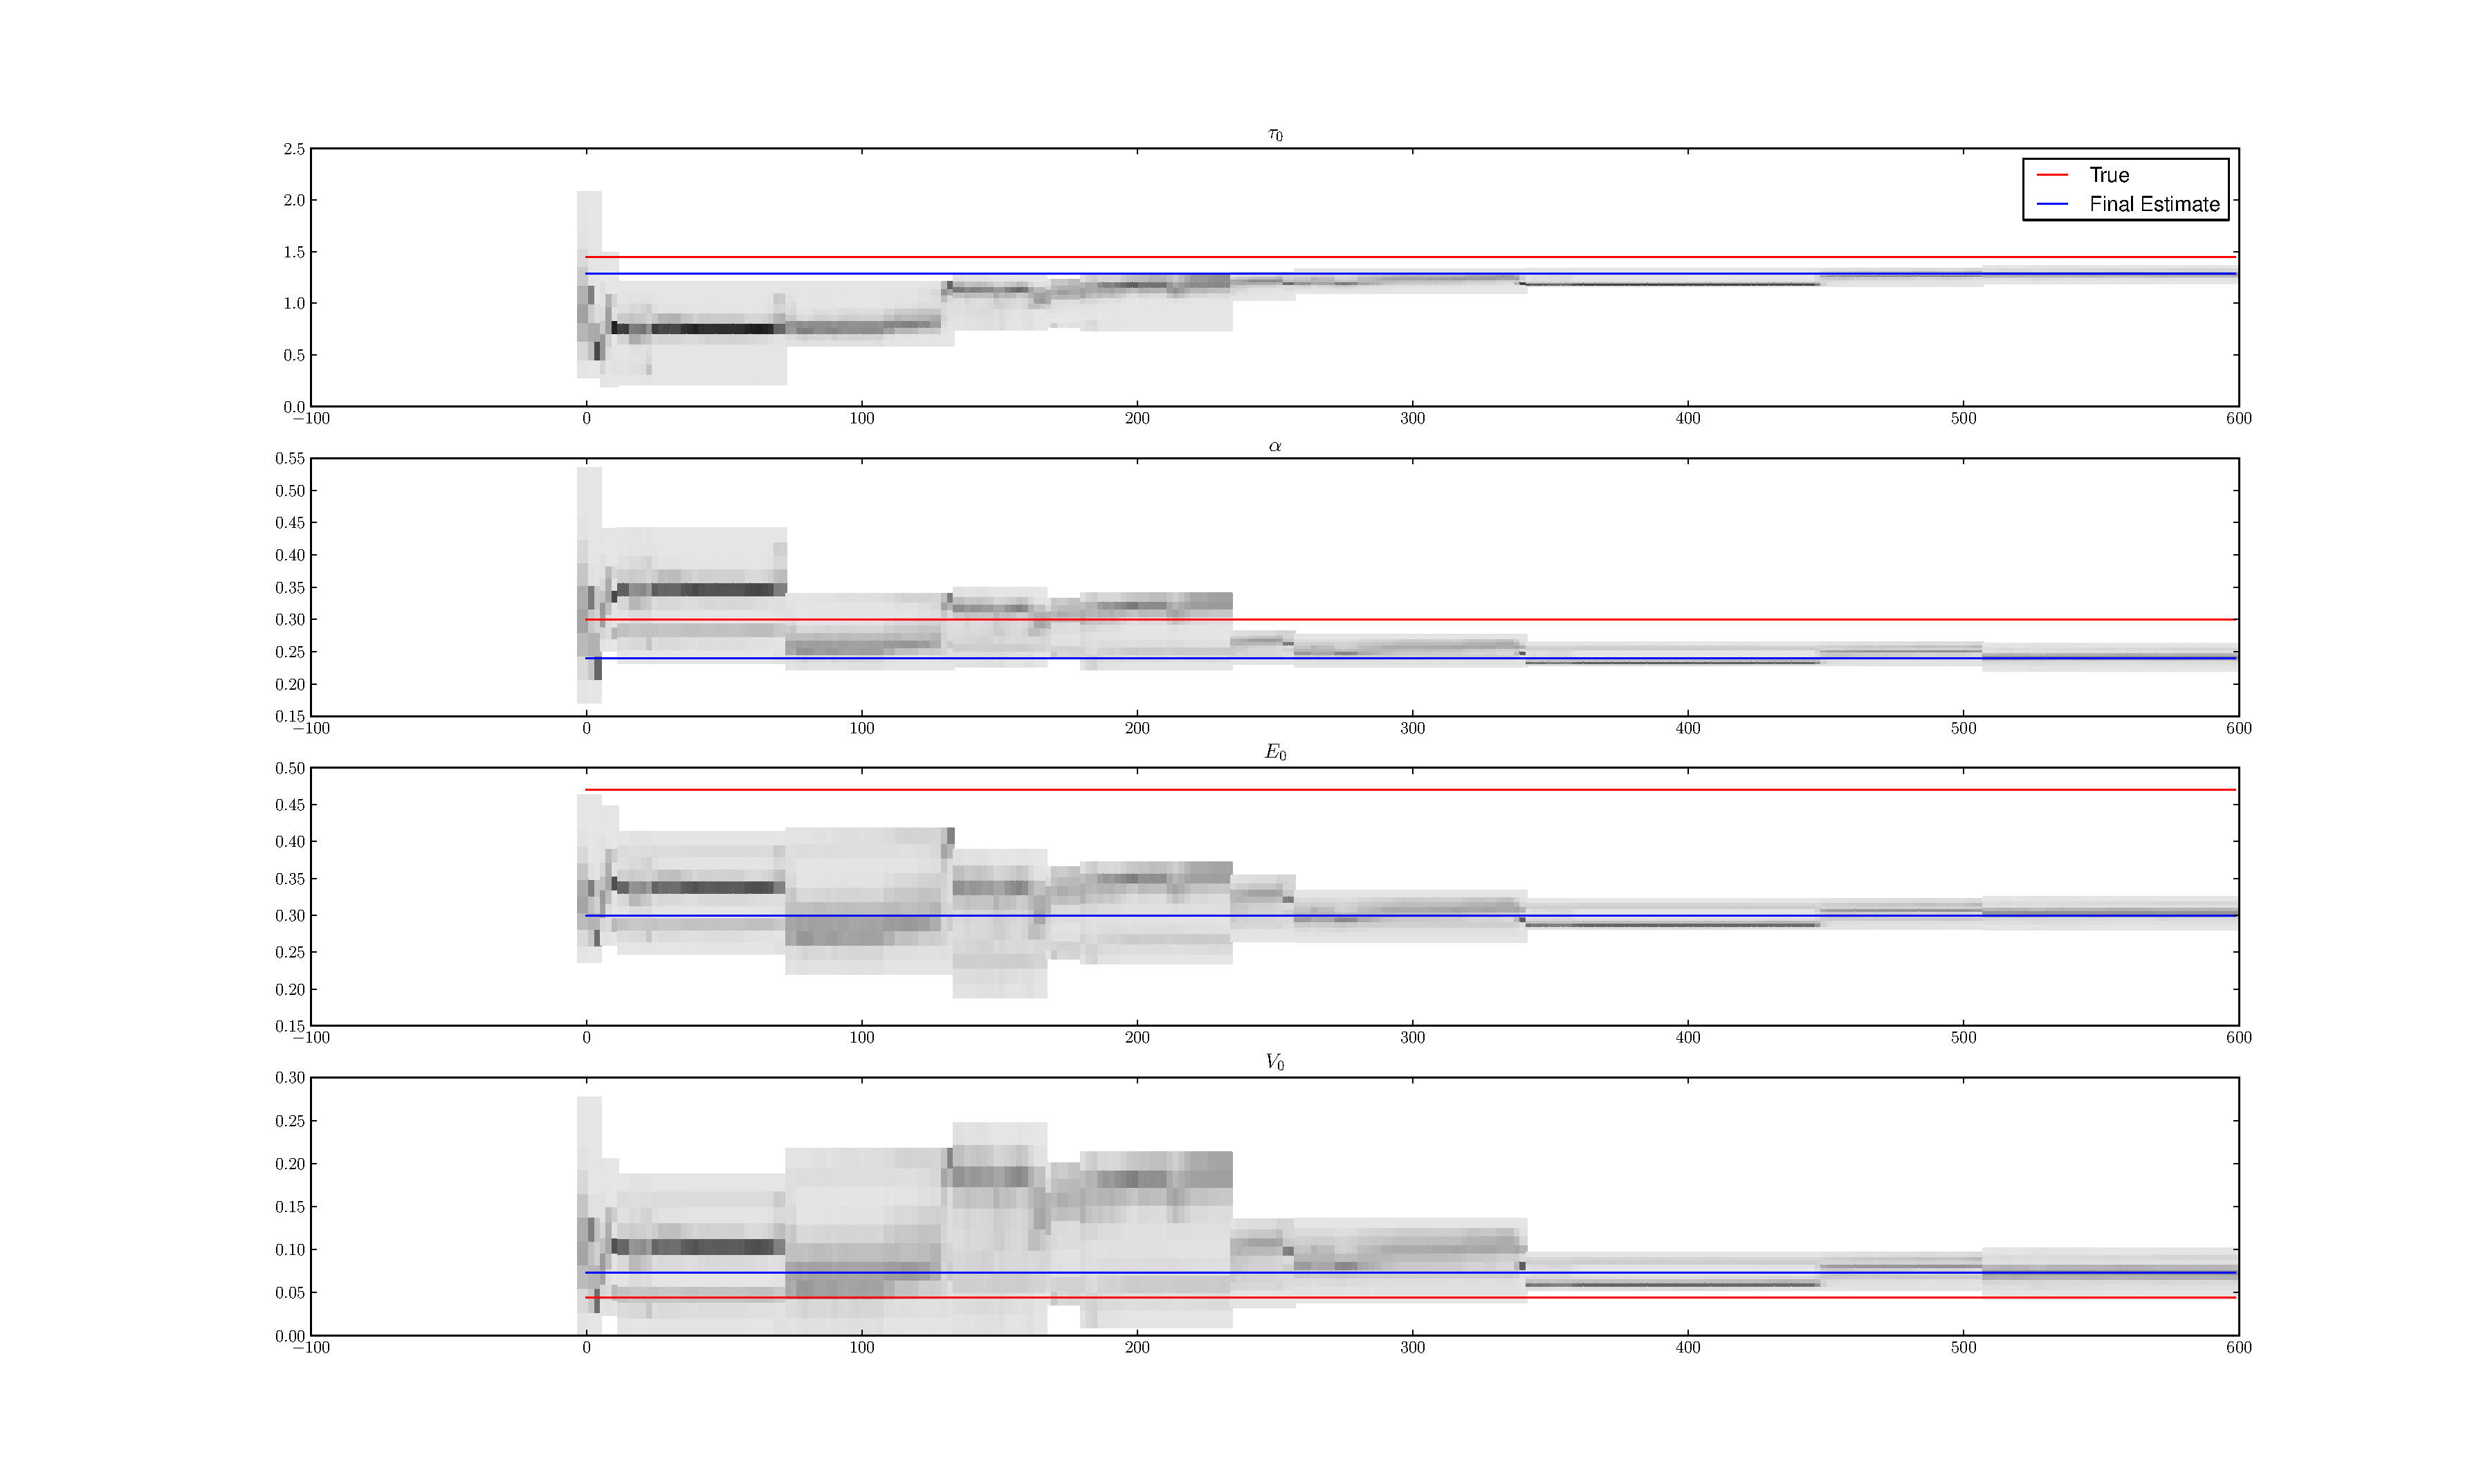
\includegraphics[clip=true,trim=6cm 3cm 6cm 3cm, height=9cm]{images/justbignoise_1}}\\
%\end{figure}
%\begin{figure}[H]
%\subfigure[$\tau_s$, $\tau_f$, $\epsilon$, $v$] 
%{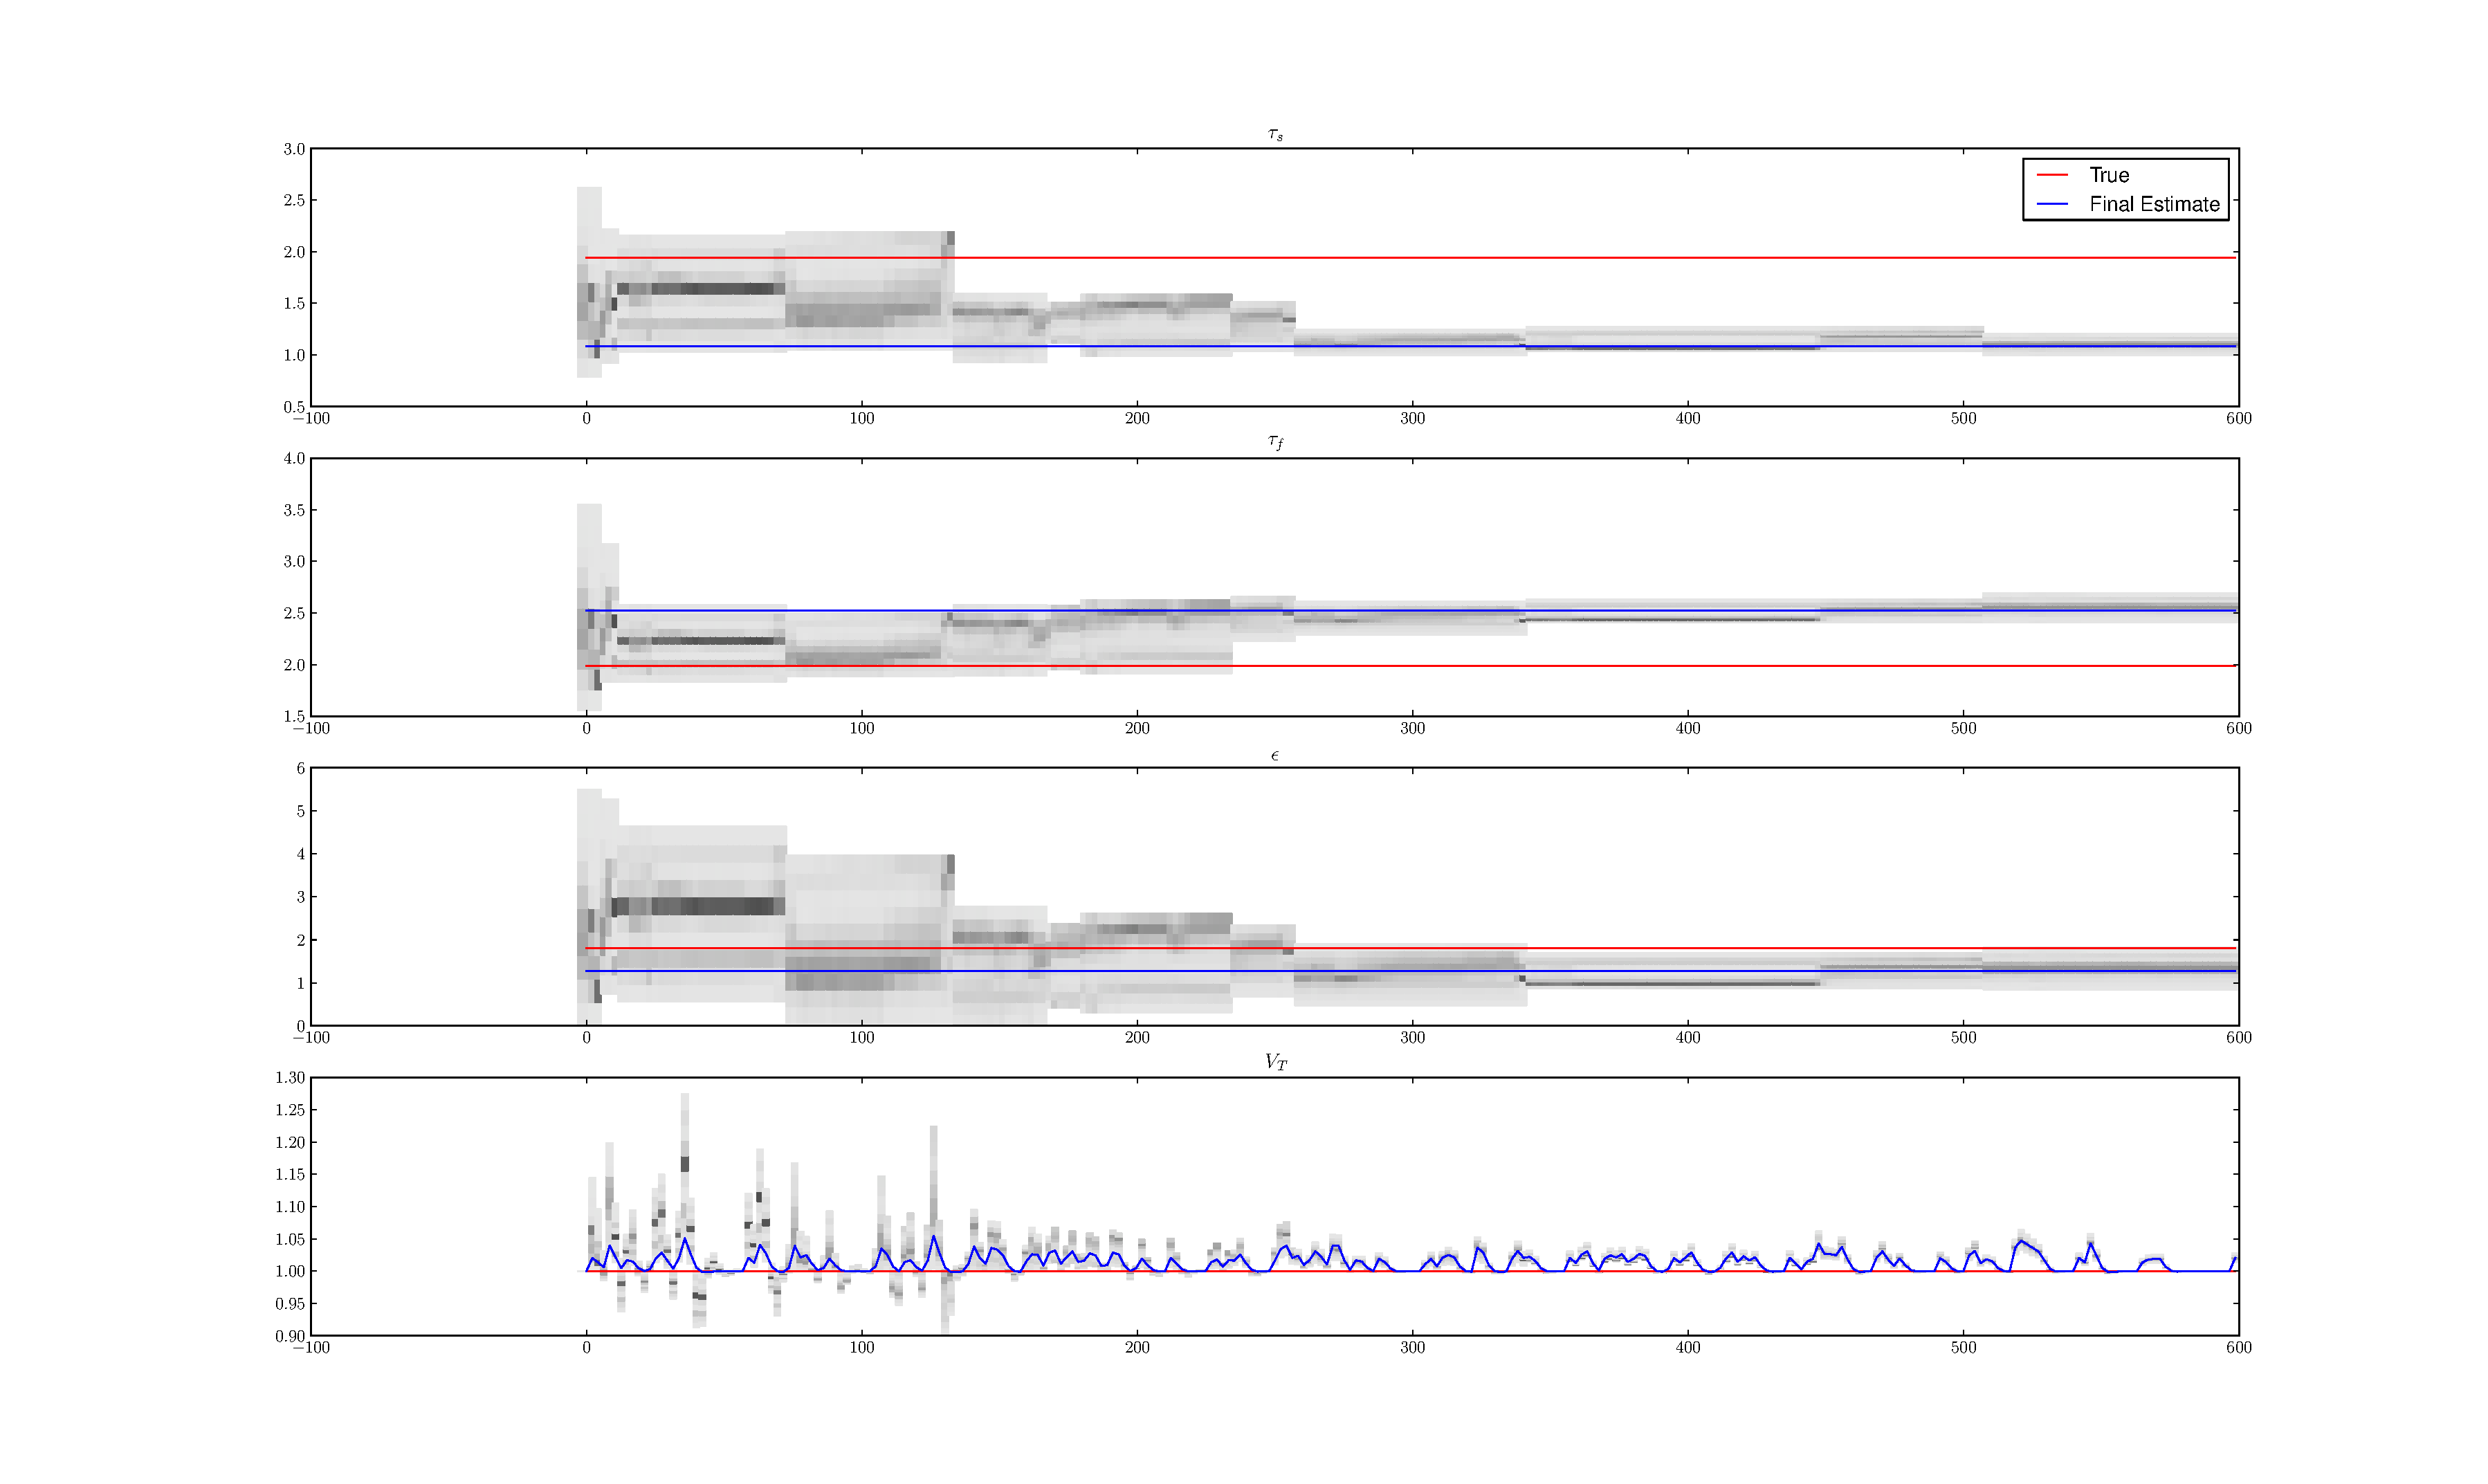
\includegraphics[clip=true,trim=6cm 3cm 6cm 3cm, height=9cm]{images/justbignoise_2}}\\
%\end{figure}
%\begin{figure}[H]
%\subfigure[$q$, $s$, $f$, $BOLD$ ]
%{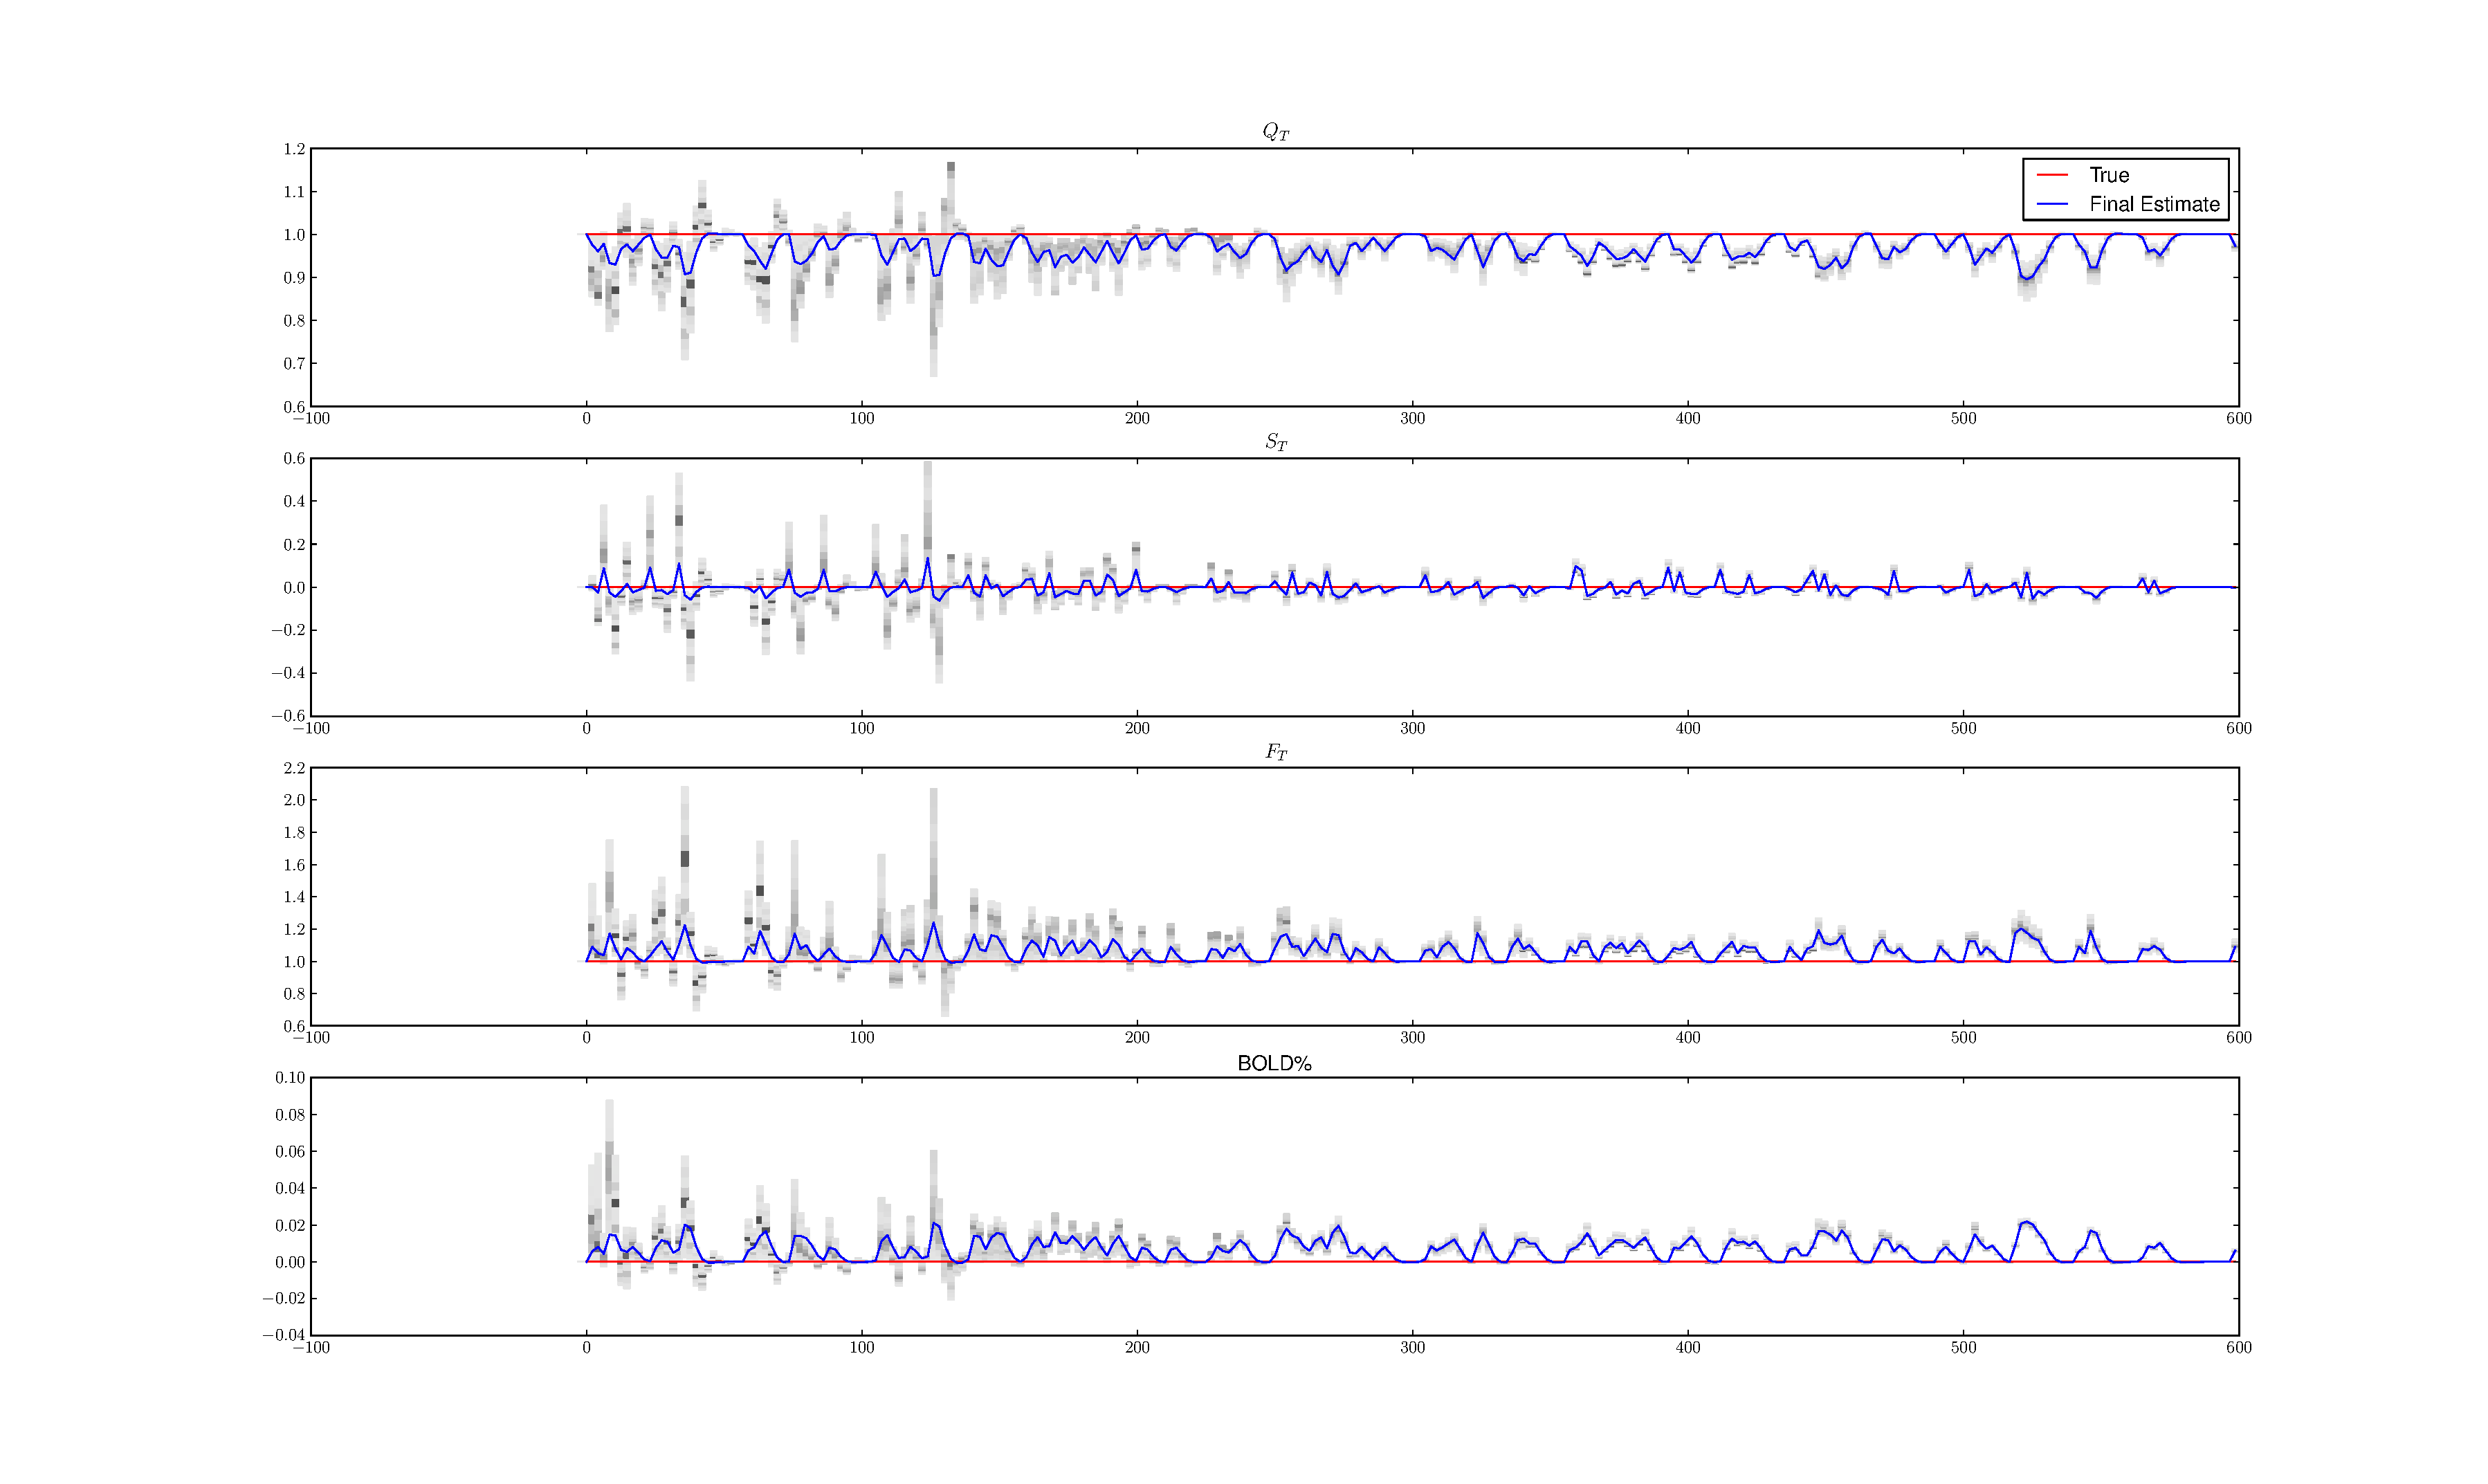
\includegraphics[clip=true,trim=6cm 3cm 6cm 3cm, height=9cm]{images/justbignoise_3}}
%\caption{Converging histogram for parameters when the signal consists purely of noise, with peaks comparable  to 
%the convential BOLD signal. ($\sigma_y = .01, \sigma_x = .005$). Same run as fit in \autoref{fig:justbignoise_fit_0}}
%\label{fig:JustNoiseConvergenceLarge}
%\end{figure}

\subsection{Single Voxel Review}
\label{sec:SingleVoxelReview}
The first step in determining the validity of a model is to provide some order of quality
to rate the results by. Unfortunately, because of the variability in the signal levels, the
raw residual cannot perform this task. As demonstrated by \autoref{tab:NoiseOnlyResults},
a low residual does not necessarily indicate a good fit. 
Therefore, instead I  normalized the signal based on a value proportional to
the magnitude of the signal. Considering the tendency of FMRI noise to have large unexplainable
peaks and troughs, rather than using MAX and MIN values to estimate the scale of the 
signal, I used a robust estimator of 
scale; the Median-Absolute-Deviation (MAD) which is defined in equation \autoref{eq:mad}.
This is an estimator of the standard
deviation, and thus a good estimator of the scale of the input signal. 
The normalized residual values are 
shown in \autoref{tab:SingleVoxelActivationComparison}. A second potential method of 
gauging performance is mutual information. Mutual information is a method of measuring
the interdependence of two random variables. If two signals are truly independent,
then the mutual information will be zero. Although ideally suited to discrete
distributions, by using histograms
it is possible to derive a joint distribution of two signals. The algorithm for 
mutual information is based on that joint distribution:
\begin{equation}
\sum_{x,y} p(x,y) \log_2\left(\frac{p(x,y)}{p(x)p(y)}\right)
\end{equation}
Unfortunately the number of bins causes bias in the output, thus to correct for this,
I subtracted the estimated bias:
\begin{equation}
\text{bias} = \frac{N_{bins}}{2Nlog(2)}
\end{equation}
where $N$ is the number of samples and $N_{bins}$ is the number of bins. For all
the mutual information estimates in this work 6 bins are used for the marginal
distribution of each signal. Additionally, throughout log base 2 will be used.
This leads to 36 total bins in the joint, so the bias is: 
\begin{equation}
\text{bias} = \frac{18}{N}
\end{equation}
 Note that subtracting the bias can result in negative mutual
information, which should not technically be possible; so any negative mutual information
was taken as 0.

\begin{table}[t]
\centering
\begin{tabular}{|c | c | c | c | c | c | c | c | c |}
\hline 
& \multicolumn{4}{|c|}{Signal} & \multicolumn{4}{|c|}{No Signal}\\
\hline
& \multicolumn{2}{|c|}{Low Noise} & \multicolumn{2}{|c|}{High Noise} 
& \multicolumn{2}{|c|}{$\sigma_y = 0.001, \sigma_x = 0.0005$} 
& \multicolumn{2}{|c|}{$\sigma_y = 0.01, \sigma_x = 0.005$}\\
\hline 
& $M.I.$ & N. Res. &
  $M.I.$ & N. Res. &
  $M.I.$ & N. Res. &
  $M.I.$ & N. Res. \\
\hline       
\hline       
1 &   0.86687  &0.47801 &  0.09077  &1.03894 &  0.06326  &  1.29501 & 0.03024  &1.33641 \\
2 &   0.93975  &0.53177 &  0.13767  &0.95165 &  -0.01075  & 1.30175 & -0.02677 &1.33667 \\
3 &   0.82382  &0.5458  &  0.13505  &0.99539 &  0.02345  &  1.26287 & -0.0111  &1.15957 \\
4 &   0.94661  &0.49824 &  0.04341  &1.16129 &  -0.00906  & 1.43196 & 0.00147  &1.09988 \\
5 &   0.94281  &0.46805 &  0.13718  &1.03972 &  0.00663  &  1.25664 & -0.00204 &1.20107 \\
6 &   0.92539  &0.459   &  0.12337  &1.00214 &  -0.00816  & 1.2708 &  0.01775  &1.04589 \\
7 &   0.98892  &0.46096 &  0.15381  &1.08847 &  0.02664  &  1.15441 & 0.03163  &1.20543 \\
8 &   0.98796  &0.51838 &  0.11325  &1.05962 &  0.03285  &  1.27456 & 0.01951  &1.1225 \\
9 &   0.8804   &0.5253  &  0.09669  &1.0157  &  0.01628  &  1.32024 & 0.01039  &1.08637 \\
10 &  0.88721   &0.49211 & 0.18339  &1.18996 &  0.00407  &  1.34456 & 0.00508  &1.22135 \\
11 &  0.96644   &0.49092 & 0.10949  &0.95368 &  0.03323  &  1.32522 & -0.01284 &1.11737 \\
\hline                                                                         
mean &0.92329  &0.49714 & 0.12037   &1.04514 &  0.01622  &  1.29437 & 0.00576  &1.17568 \\
\hline                                                                           
min &  0.82382  &0.459   &  0.04341  &0.95165 & -0.01075  & 1.15441 & -0.02677 &1.04589 \\
\hline                                                                         
max &  0.98892  &0.5458  & 0.18339   &1.18996 & 0.06326  &  1.43196 & 0.03163  &1.33667 \\
\hline
\end{tabular}
\caption{Mutual Information and the normalized $\sqrt{MSE}$, 
    for signal/noise configurations.}
\label{tab:SingleVoxelActivationComparison} 
\end{table}


Comparing the results of \autoref{sec:SimHighNoise} and \autoref{sec:PureNoiseHighMag} 
in \autoref{tab:SingleVoxelActivationComparison}, 
distinguishing between these cases with ether normalized residual or mutual information
is not clear cut. While the average mutual information is in fact more than 10 times
the average mutual information in the two non-signal cases, the maximum
mutual information of the low noise/no signal case exceeds the minimum M.I. of the high noise/signal
case. The Low Noise/ signal determination is easier to make; given
the minimum mutual information is above $.8$ and the maximum normalized residual is below $.6$.
However, it is worth noting that the worst case scenario  for mutual information (maximum) in the
low noise/no signal case does not concur with the worse case (minimum) normalized residual. 
There is no reason why this has to be the case, but it is beneficial. In
other words, if it were necessary to make a statement that
a particular voxel were active or inactive; the accuracy would improve if both techniques
were used with loose restrictions.

There were two primary purposes of these tests. First, given the nature of monte-carlo
techniques it is important to ensure consistency of results. Although the parameter
sets were inconsistent, the quality of the fit was actually quite consistent
over eleven runs. The second purpose was of course to determine how the particle 
filter responded to different signal to noise ratios. From \autoref{sec:SimLowNoise},
the particle filter performed extremely well in filtering out nonsensical measurements.

\section{Multi-voxel Simulation}
\label{sec:Multi-voxel Simulation}
To test the usefulness of the particle filter on a larger scale, I used a modified version 
of the FSL tool 
POSSUM to generate an entire FMRI image from a parameter map. The parameter map was generated
by taking an existing activation map and assigning discrete parameter sets to each region.
The result was a four dimensional (length x width
x height x parameter) image with spatially varying parameters. Possum was then modified
to take a parameter map and generate activation levels depending on the parameters at that
point. The patch for POSSUM will be made available. It is worth noting is that the noise 
level was set to an SNR of 20, but due to changes 
in the program the true signal-to-noise ratio was much lower, as seen in the 
in \autoref{fig:SimSNRhm}. The mean SNR for each region was calculated only for the
voxels with a Signal-To-Noise ratio above $0.1$.

\begin{figure}
\centering
\subfigure{
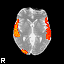
\includegraphics[width=10cm]{images/snr_hm.png}}
\subfigure{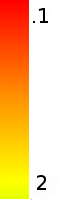
\includegraphics[width=1cm]{images/scale5.png}}
\caption{SNR Map of POSSUM simulated data. Region 1 mean SNR was $0.8$, Region 2 mean SNR was $0.97$, and 
Region 3 mean SNR was $0.39$.}
\label{fig:SimSNRhm}
\end{figure}

For each time-series in the simulated FMRI image, the final parameters were saved
into a parameter map. This parameter map could then be compared to the map used to generate the 
simulated data; additionally a new simulation using the calculated parameters could also be 
generated to test the difference in BOLD levels between the real parameters and the
estimated ones. Since the parameters were far from orthogonal 
\cite{Deneux2006}, this provided a quantitative difference between the two parameter sets.

\begin{figure}[H]
\centering
\subfigure[Region labels for simulated slice.]{
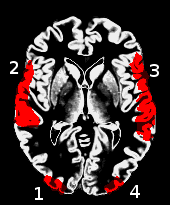
\includegraphics[height=9.5cm]{images/simregions.png} \label{fig:simslice_mask} }
\subfigure[Grey matter map for simulate region.]{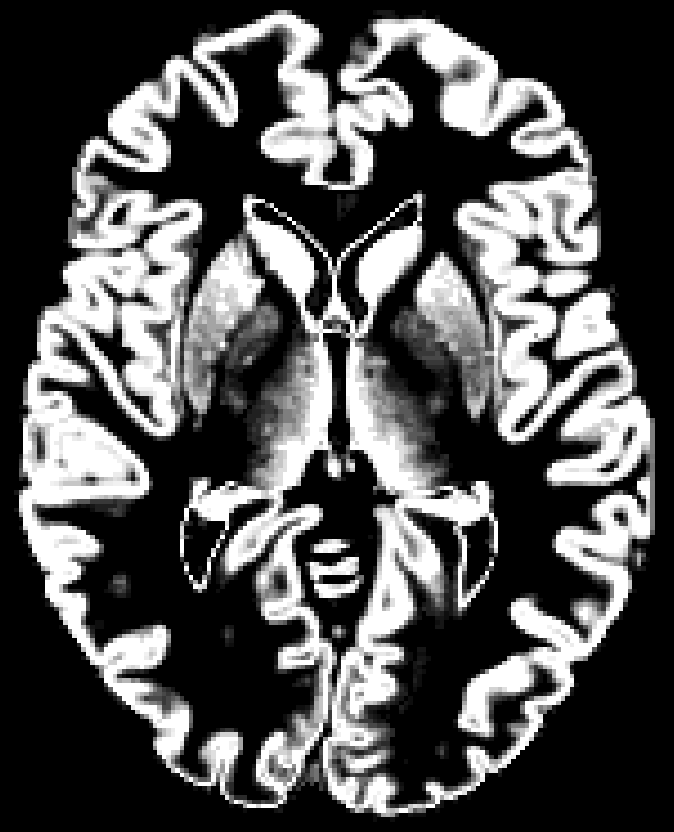
\includegraphics[height=9.5cm]{images/sim_gm}}
\subfigure[Residual Map. Scale is Normalized $\sqrt{MSE}$. Lower (yellow) is better.]
{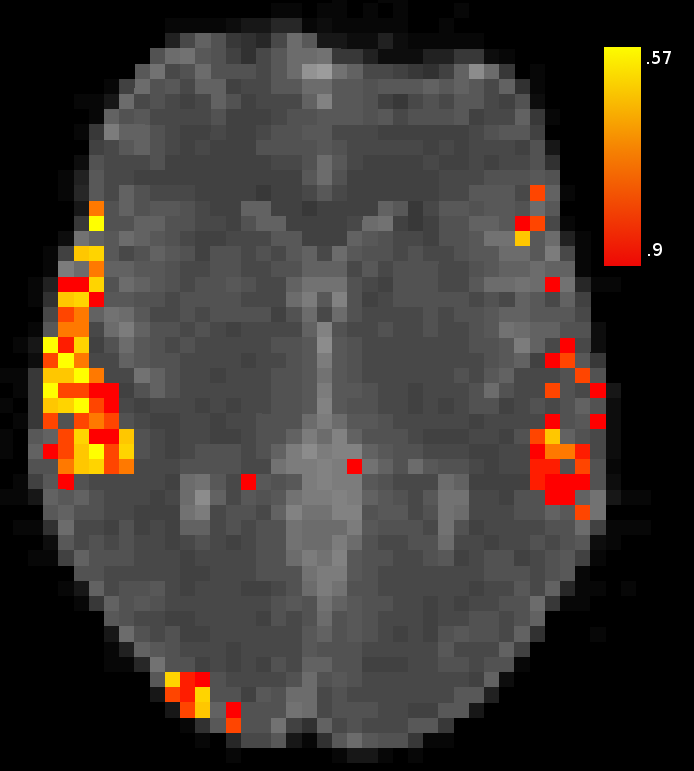
\includegraphics[height=9cm]{images/sim_hm}}
\subfigure[Mutual Information Map. Scale is bits. Higher (yellow) is better.]
{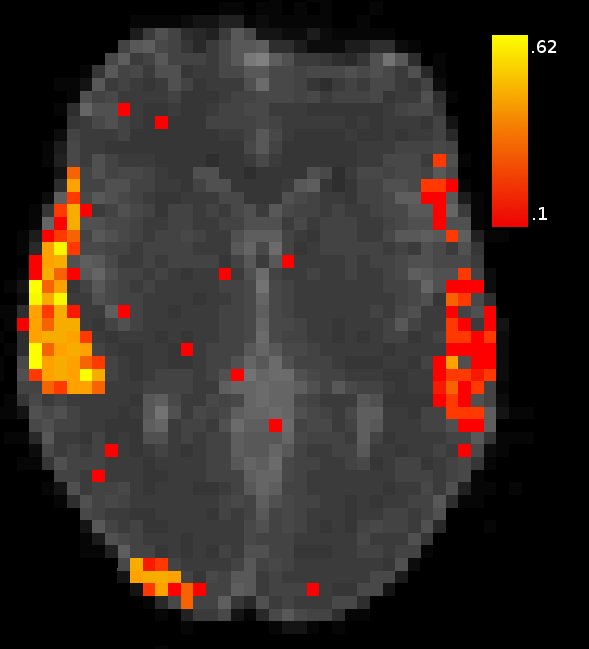
\includegraphics[height=9cm]{images/sim_hm_mi}}
\caption{Comparison of activation with greymatter, parameter regions.}
\label{fig:simslice_hm}
\end{figure}

The regions are numbered according to \autoref{fig:simslice_mask}; the parameters
for each region may be found in \autoref{tab:simsliceparams}. 

\begin{table}[t]
\centering
\begin{tabular}{|c |c | c | c | c | c | c | c |}
\hline 
Region & $\tau_0$ & $\alpha$ & $E_0$    & $V_0$    & $\tau_s$ & $\tau_f$ & $\epsilon$  \\
\hline 
1 & 1.454& 0.321& 0.369& 0.036& 0.994& 2.774& 1.348\\
2 &1.151&  0.353& 0.380& 0.026& 1.98&  2.333& 1.645 \\
3 &1.951&  0.317& 0.348& 0.027& 1.657& 3.719& 0.757 \\
4 &1.203 & 0.310& 0.326& 0.036& 2.168& 2.272& 0.086\\
\hline
\end{tabular}
\caption{Actual parameters for each regions in the simulated slice.}
\label{tab:simsliceparams} 
\end{table}

Note that region 4 has a very low $\epsilon$. For this reason, the only areas
with significant estimates of the BOLD time series were 1,2 and 3. With
such a low $\epsilon$, region 4 was below the noise threshold. Notice that the
regions 1, 2 an 3 stick out in both the residual and the mutual information
map, indicating that the particle filter was successful in matching those regions. 
Mutual information was an extremely succesfull metric, with the exception of 
a few false positives. Thus, another heatmap (\autoref{fig:sim_hm2}) is 
helpful to show what threshold would remove those false positives. 

\begin{figure}
\centering
\subfigure{
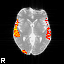
\includegraphics[width=10cm]{images/sim_hm_15_6.png}}
\subfigure{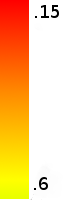
\includegraphics[width=1cm]{images/scale6.png}}
\caption{More stringent mutual information heatmap. Higher (yellow) is better.}
\label{fig:sim_hm2}
\end{figure}

\begin{figure} %bottom left
\centering
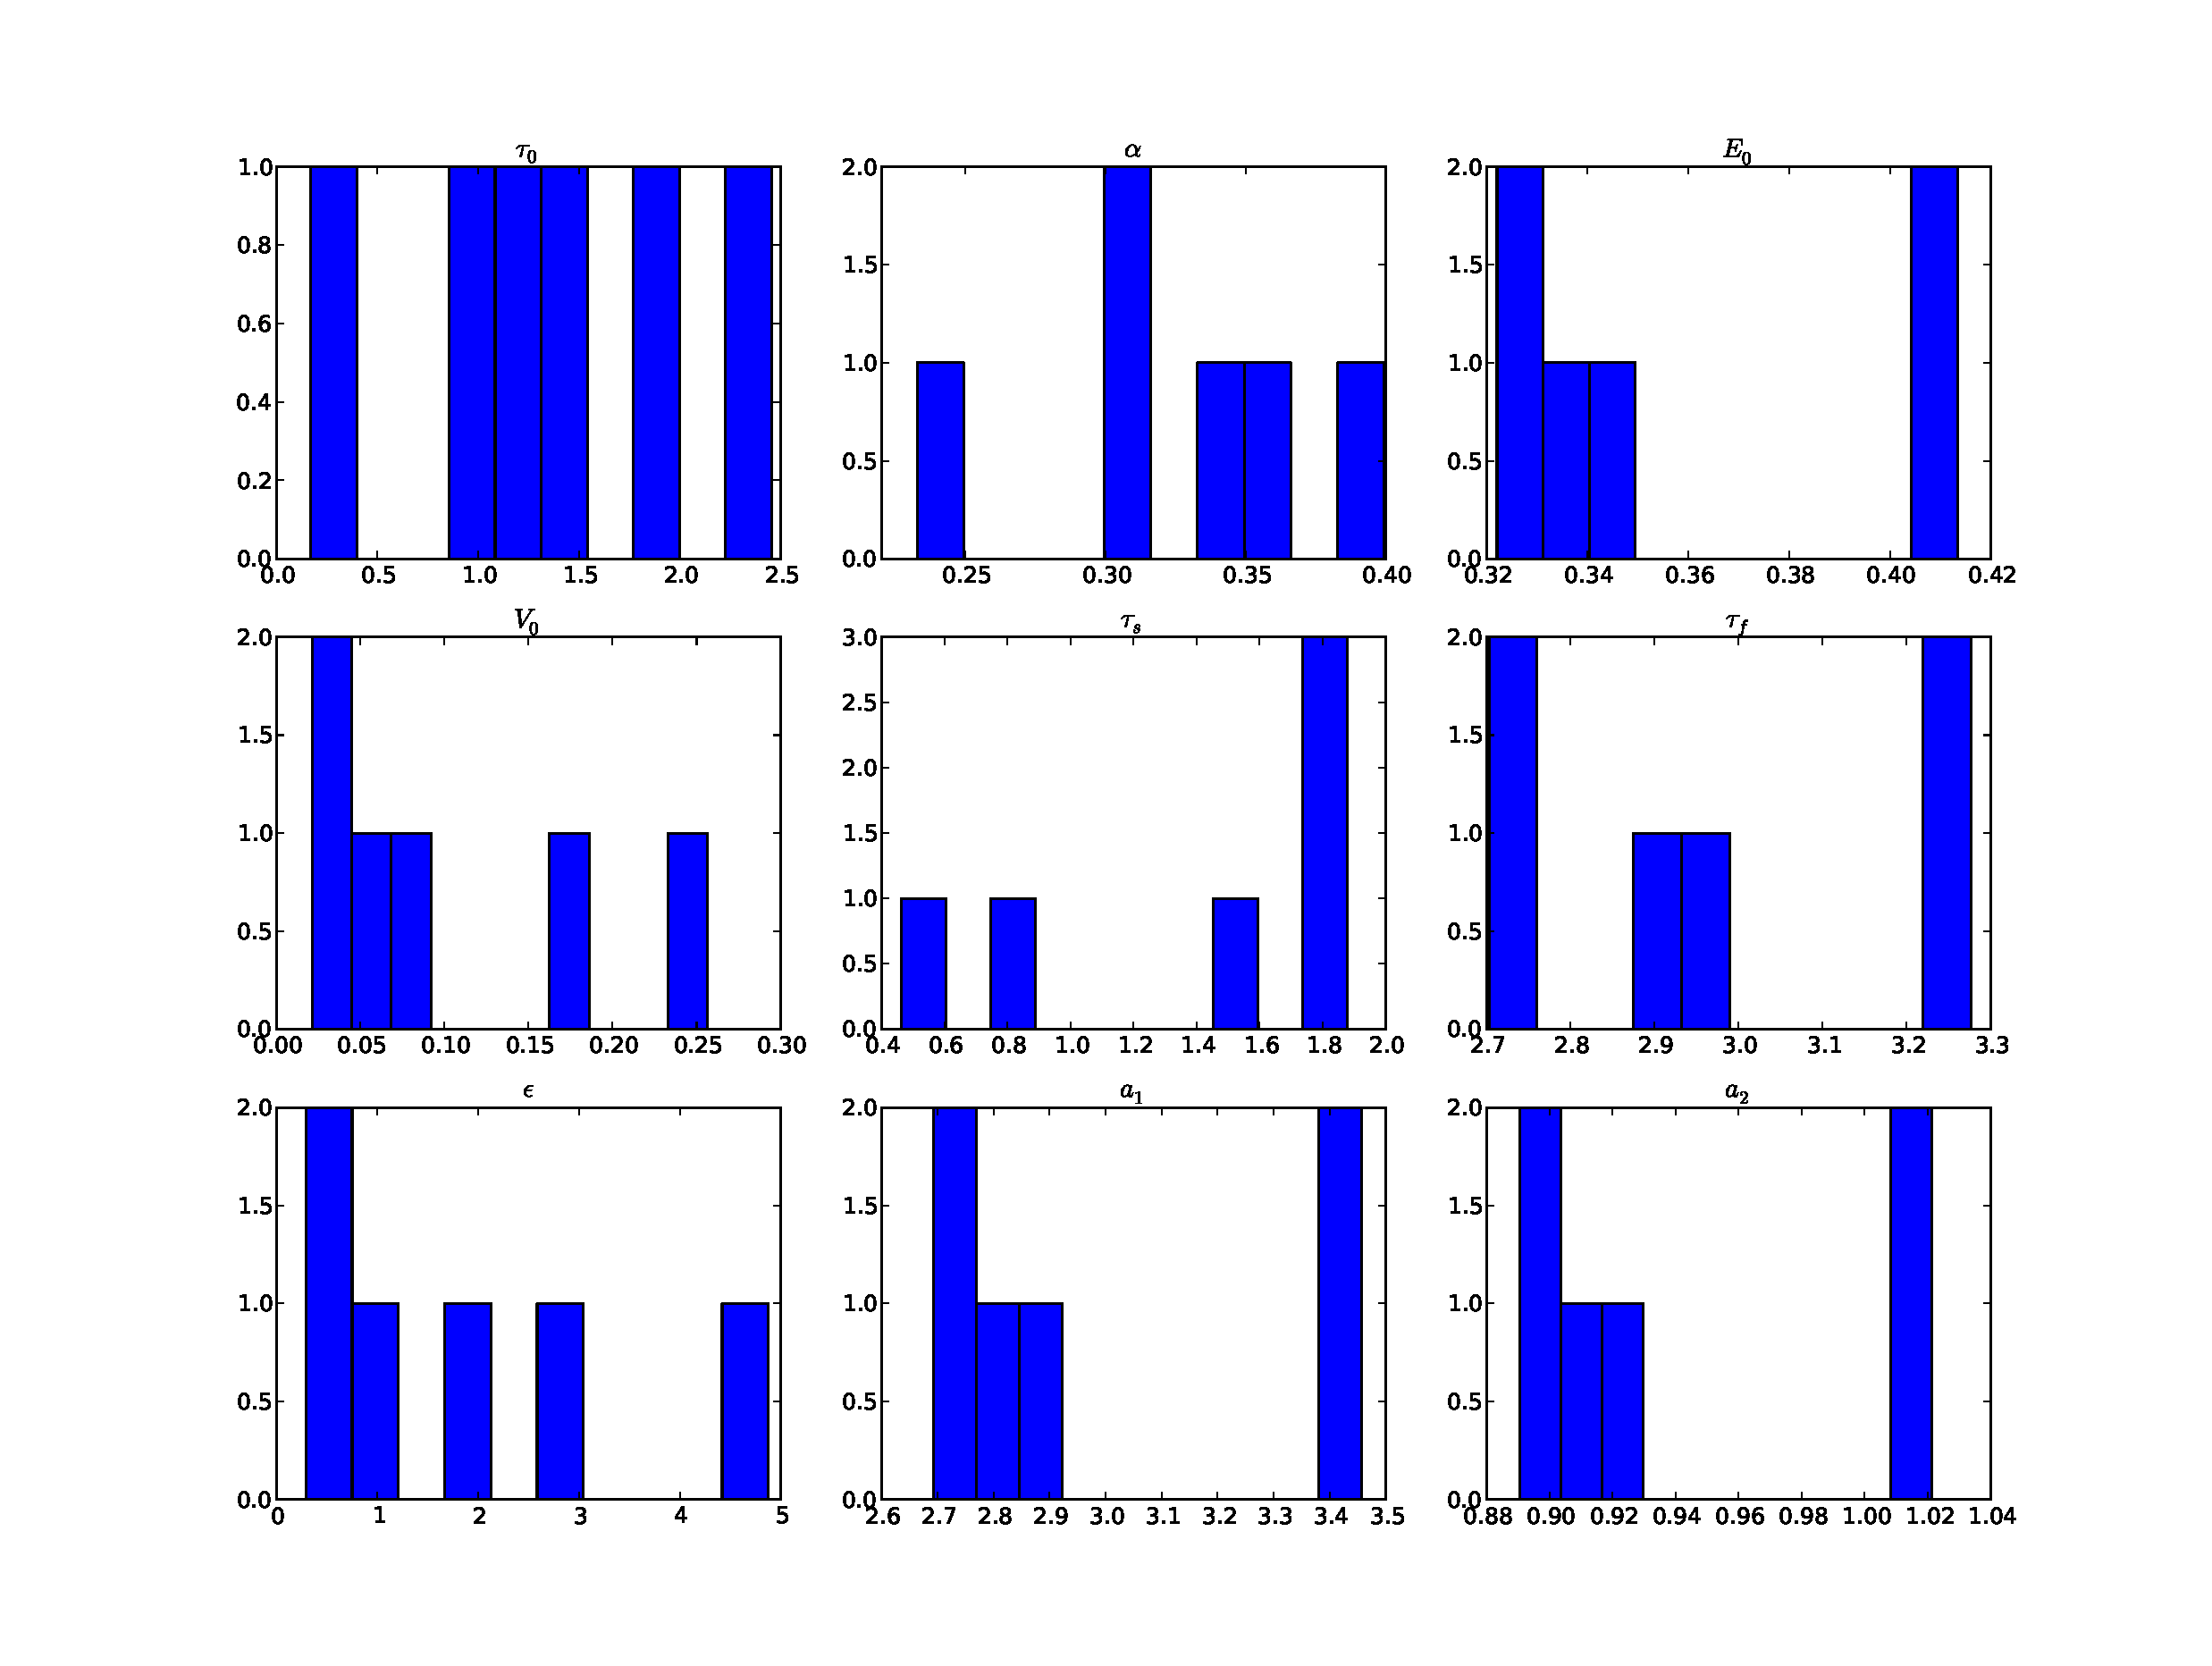
\includegraphics[clip=true,trim=2.5cm 2cm 2cm 1cm,width=15cm]{images/slicesim_hist1}
\caption{Histogram of estimated parameters in section 1 in voxels with mutual information greater
than $0.14$}
\label{fig:slicesim_hist1}
\end{figure}

\begin{figure} %top left
\centering
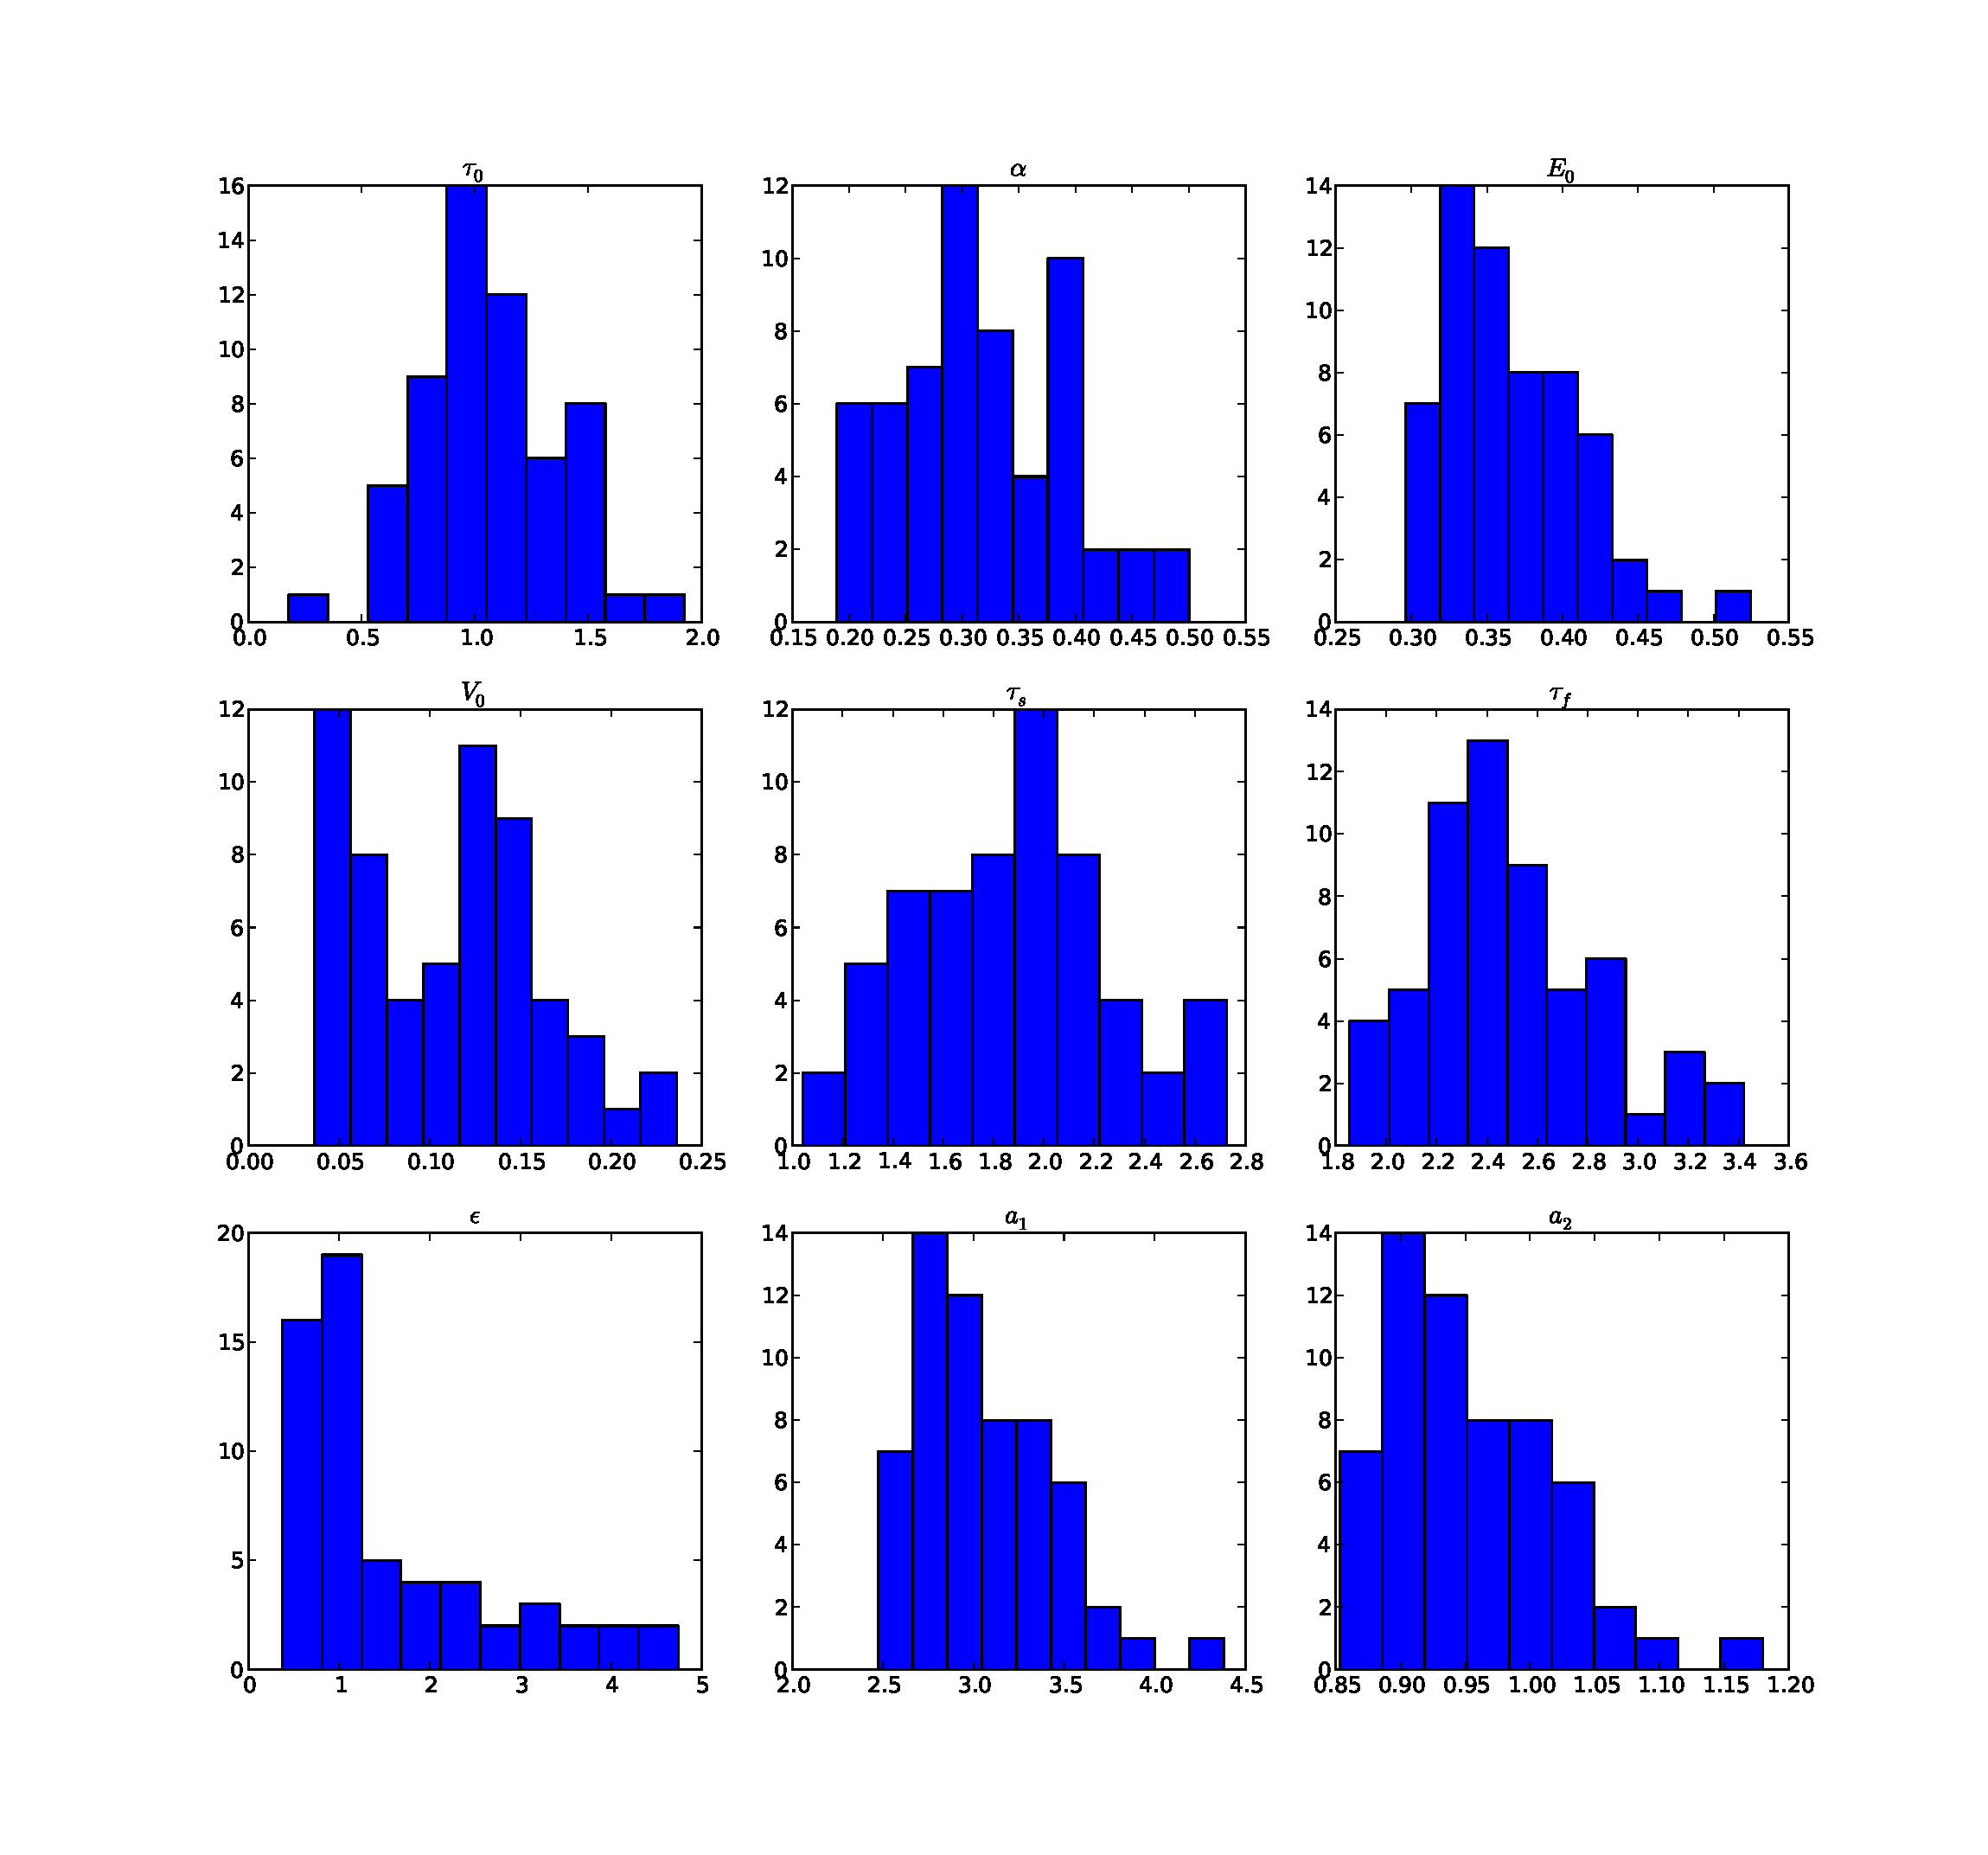
\includegraphics[clip=true,trim=2.5cm 2cm 2cm 1cm,width=15cm]{images/slicesim_hist2}
\caption{Histogram of estimated parameters in section 2 in voxels with mutual information greater
than $0.14$}
\label{fig:slicesim_hist2}
\end{figure}

\begin{figure} %top right
\centering
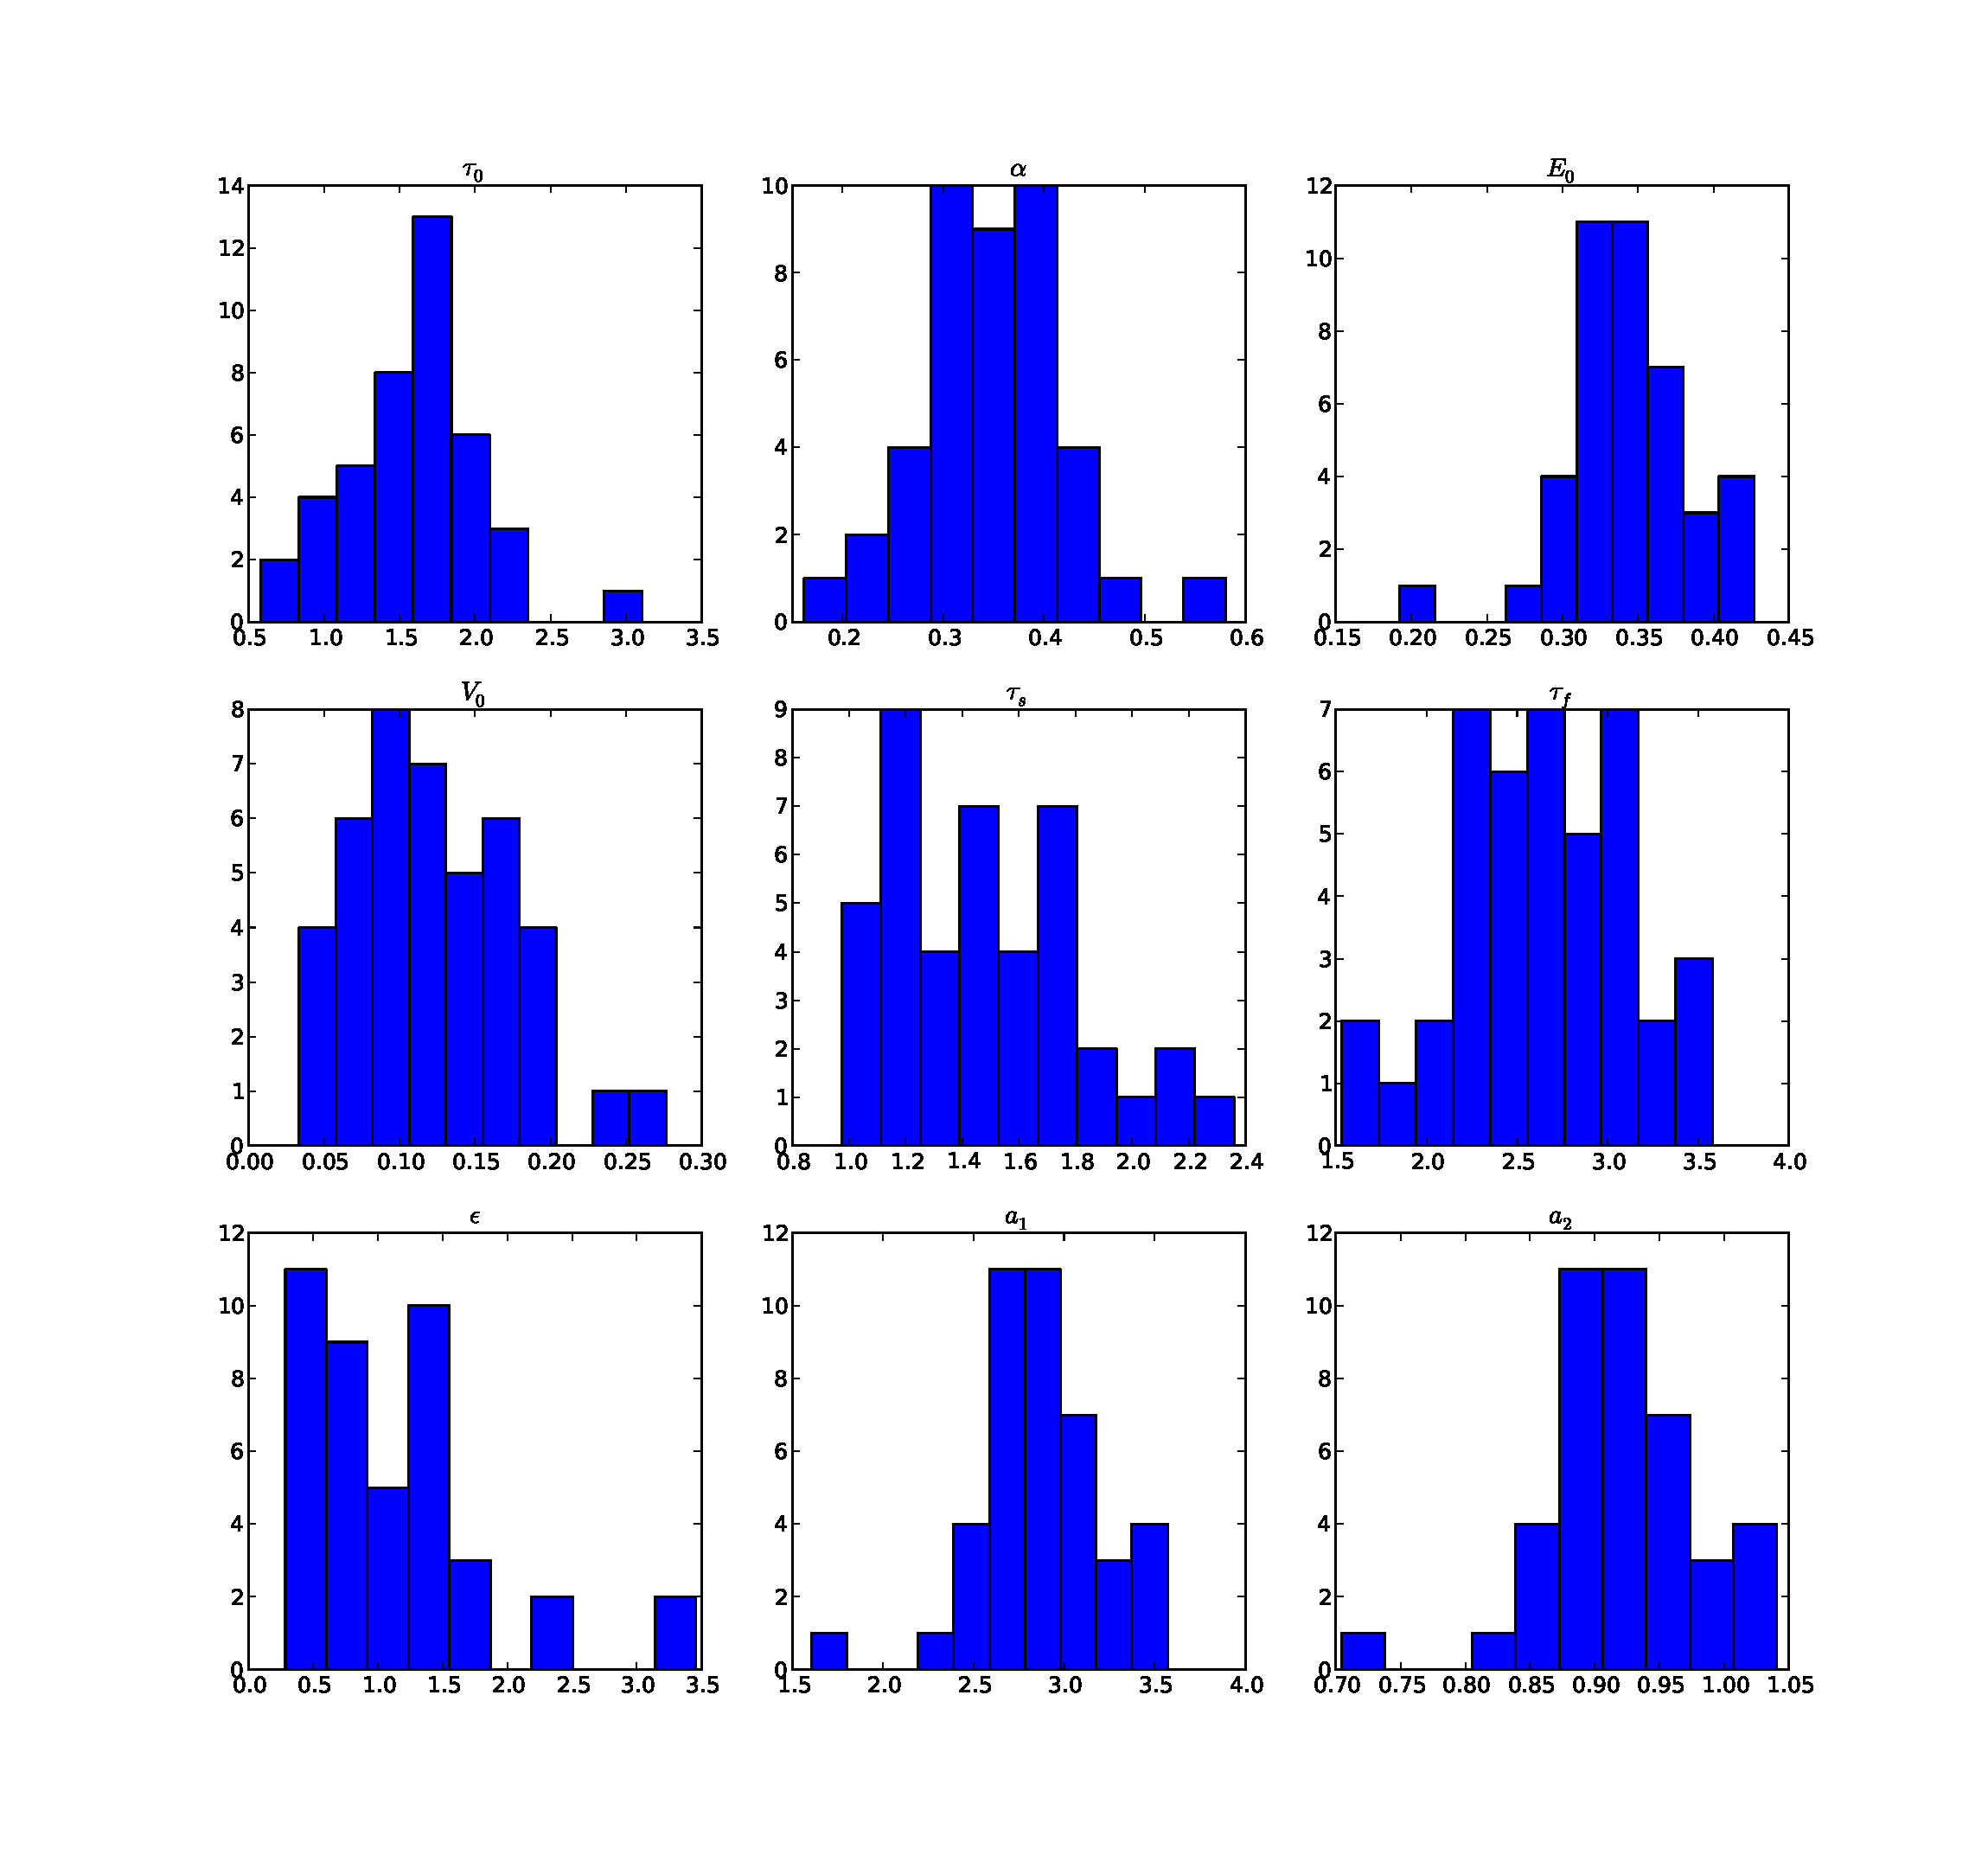
\includegraphics[clip=true,trim=2.5cm 2cm 2cm 1cm,width=15cm]{images/slicesim_hist3}
\caption{Histogram of estimated parameters in section 3 in voxels with mutual information greater
than $0.14$}
\label{fig:slicesim_hist3}
\end{figure}

The histograms again demonstrate that a single point estimate of the parameters 
is elusive for this set of parameters. However the data clearly show the power
of the particle filter at identifying regions of activation; which is usually
performed with statistical parametric maps. The thresholds applied to this
slice, both for mutual information and residuals is arbitrary, and needs further
research. Tighter thresholds removes the false positives present
in the images at the cost of false negatives. As noted in \autoref{sec:SingleVoxelReview}
the false positives present in the Mutual Information
map are different from those in the residual map. This furthers the argument from
for combining the two metrics to increase power. Although
at first glance it would appear that there are false negatives in the 
\autoref{fig:simslice_hm}; this is
not actually the case. POSSUM simulates different tissues, and white matter
does not typically  have a BOLD response. This is why there are holes in regions
2 and 3. These results indicate that the particle filter is effective
at regressing against a noisy signal. 
